% Typical processing for PostScript (PS) output:
%
%  latex advanced_example
%  bibtex advanced_example  (bibliography)
%  makeindex -s nomencl.ist -o advanced_example.gls advanced_example.glo
%                            (nomenclature)
%  latex advanced_example   (repeat as needed to resolve references)
%
%  xdvi advanced_example    (onscreen draft display)
%  dvips advanced_example   (postscript)
%  gv advanced_example.ps   (onscreen display)
%  lpr advanced_example.ps  (hardcopy)
%
% With the above, only Encapsulated PostScript (EPS) images can be used.
%
% Typical processing for Portable Document Format (PDF) output:
%
%  pdflatex advanced_example
%  bibtex advanced_example    (bibliography)
%  makeindex -s nomencl.ist -o advanced_example.gls advanced_example.glo
%                              (nomenclature)
%  pdflatex advanced_example  (repeat as needed to resolve references)
%
%  acroread advanced_example.pdf  (onscreen display)
%
% If you have EPS figures, you will need to use the epstopdf script
% to convert them to PDF because PDF is a limmited subset of EPS.
% pdflatex accepts a variety of other image formats such as JPG, TIFF,
% PNG, and so forth -- check the documentation for your version.
%
% If you do *not* specify suffixes when using the graphicx package's
% \includegraphics command, latex and pdflatex will automatically select
% the appropriate figure format from those available.  This allows you
% to produce PS and PDF output from the same LaTeX source file.
%
% To generate a large format (e.g., 11"x17") PostScript copy for editing
% purposes, use
%
%  dvips -x 1467 -O -0.65in,0.85in -t tabloid advanced_example
%
% For further details and support, read the Users Manual, aiaa.pdf.



\documentclass[]{aiaa-tc}% insert '[draft]' option to show overfull boxes

 \usepackage{varioref}%  smart page, figure, table, and equation referencing
 \usepackage{wrapfig}%   wrap figures/tables in text (i.e., Di Vinci style)
 \usepackage{threeparttable}% tables with footnotes
 \usepackage{dcolumn}%   decimal-aligned tabular math columns
  \newcolumntype{d}{D{.}{.}{-1}}
 \usepackage{nomencl}%   nomenclature generation via makeindex
  \makeglossary
 \usepackage{subfigure}% subcaptions for subfigures
 \usepackage{subfigmat}% matrices of similar subfigures, aka small mulitples
 \usepackage{fancyvrb}%  extended verbatim environments
  \fvset{fontsize=\footnotesize,xleftmargin=2em}
 \usepackage{lettrine}%  dropped capital letter at beginning of paragraph
 \usepackage[dvips]{dropping}% alternative dropped capital package
 \usepackage[colorlinks]{hyperref}%  hyperlinks [must be loaded after dropping]


%%%%% Title %%%%%
 \title{Multi-species Fluid Flow Simulations using a Hybrid Computational Fluid Dynamics - Molecular Dynamics Appraoch 
 \skonote{Or "Polyatomic Lagrangian Dynamics Modelling for a Hybrid Computational Fluid Dynamics - Molecular Dynamics Appraoch"} }
%%%%% End Title %%%%%


%%%%% Author %%%%%
 \author{
  Nayong Kim\thanks{A Post-doctoral Researcher; Center for Computation \& Technology,
  Louisiana State University, Baton Rouge, LA 70803, USA; Non-AIAA Member}\\
  {\normalsize\itshape
   Louisiana State University, Baton Rouge, LA 70803, USA}\\
  \and
  Soon-Heum Ko\thanks{A Computational Scientist; National Supercomputing Centre,
  Link\"{o}ping University, Link\"{o}ping, 581 83 Sweden; Non-AIAA Member}\\
  {\normalsize\itshape
   Link\"{o}ping University, Link\"{o}ping, 581 83, Sweden}\\
  \and
  Shantenu Jha\thanks{An Assistant Professor; Department of Electrical and Computer Engineering,
  94 Brett Road, Piscataway, NJ 08854, USA; Non-AIAA Member}\\
  {\normalsize\itshape
   Rutgers University, Piscataway, NJ 08854, USA}\\
  \and
  Dorel Moldovan\thanks{An Associate Professor; Department of Mechanical Engineering,
  Louisiana State University, Baton Rouge, LA 70803, USA; Non-AIAA Member}
    \ and
  Dimitris E. Nikitopoulos\thanks{A Professor; Department of Mechanical Engineering,
  Louisiana State University, Baton Rouge, LA 70803, USA; AIAA Member}\\
  {\normalsize\itshape
   Louisiana State University, Baton Rouge, LA 70803, USA}\\
 }
%%%%% End Author %%%%%


 % Data used by 'handcarry' option
 \AIAApapernumber{YEAR-NUMBER}
 \AIAAconference{Conference Name, Date, and Location}
 \AIAAcopyright{\AIAAcopyrightD{YEAR}}

 % Define commands to assure consistent treatment throughout document
 \newcommand{\eqnref}[1]{(\ref{#1})}
 \newcommand{\class}[1]{\texttt{#1}}
 \newcommand{\package}[1]{\texttt{#1}}
 \newcommand{\file}[1]{\texttt{#1}}
 \newcommand{\BibTeX}{\textsc{Bib}\TeX}


%%%%% Note Configuration %%%%%
\newcommand{\jhanote}[1]{ {\textcolor{red} { ***Jha: #1 }}}
\newcommand{\Nkimnote}[1]{ {\textcolor{blue} { ***NKim: #1 }}}
\newcommand{\skonote}[1]{ {\textcolor{green} { ***Jeff: #1 }}}
\newcommand{\menote}[1]{ {\textcolor{purple} { ***Comment from ME: #1 }}} 
%%%%% End Note Configuration %%%%%


\begin{document}

\maketitle


%%%%% Abstract %%%%%
\begin{abstract}
\skonote{Before going further, check the AIAA membership on co-authors: basically Dimitris is most likely to own the membership}
The constrained Lagrangian dynamics modelling in the hybrid computational fluid dynamics (CFD) - molecular dynamics (MD) approach is improved for the simulation of multi-species polyatomic fluid.
Microscopic mean velocity term on the classical Lagrangian dynamics equation is replaced by the division of mean linear momentum and mean mass to account for multi-species fluid system.
Also, the equation is applied on molecules instead of individual atom, to preserve the linear momentum between continuum and particle domain without encountering the unfaborable numerical break-down of molecular structure.
We verify our hybrid CFD-MD simulation package by analyzing a nano-scale transient Couette flow of a single monatomic fluid.
We will evaluate the multi-species polyatomic Lagrangian dynamics modelling by analyzing two different fluid models: the mixture of two monatomic fluids and a polyatomic molecular fluid under the short-range potential.
These two applications will describe the effect of particle-level mass variation on the macroscopic flow evolution.
\end{abstract}
%%%%% End Abstract %%%%%


%\printglossary %creates nomenclature section produced by MakeIndex


%%%%% Introduction %%%%%
\section{Introduction}
\label{sec:intro}

\lettrine[nindent=0pt]{T}{he} hybrid computational fluid dynamics (CFD) - molecular dynamics (MD) approach is getting more attraction as a potential answer in accurately describing the nano-scale flow phenomena in the range of an acceptable computational cost.




A hybrid continuum dynamics - particle dynamics approach is an approach 
capable of describing accurately a flow at both macroscopic and molecular scales. 
In this approach the system is divided into two domains. 
A continuum formulation is used appropriately for one domain and 
a particle formulation (e.g. molecular dynamics) is applied to the other.
Naturally the particle domain is more appropriate for material interfaces 
(e.g. fluid/solid or fluid/fluid) where molecular effects are more likely to be important. 
On the other hand, the continuum approach provides a better computational efficiency than
particle dynamics with acceptable accuracy in solving the bulk flow field.
In the hybrid approach the two domains are coupled through an overlap region/interface 
in which both formulations are valid. The overlap domain enables the exchange of 
conservative flow properties between the continuum and particle ones so that 
the respective solutions are mutually consistent. 
The information from the continuum domain is passed to the particle domain 
by imposing additional numerical modeling to preserve higher degree-of-freedom 
on the particle motion, while the particle domain provides boundary conditions 
to the continuum domain obtained through time and spatial averaging of the relevant variable.

Despite the recent developments reported in the literature, most of which tested 
against small idealized pure atomistic flow simulations for comparison, 
there are still methodological and implementation issues that need refinement, 
testing and validation. In this section, we will give a brief account of the numerical and 
computational issues associated with some of the previous hybrid CFD-MD implementations 
and outline our approach to address them effectively.


\subsection{Previous Hybrid CFD-MD Implementations}
\label{sec:intro_formerworks}
%Hybrid simulation approaches can be grouped into two according to the microscopic solution method coupled into macroscopic continuum domain.~\cite{Koumoutsakos} One is the coarse-grained particle simulations by using Direct Simulation Monte Carlo (DSMC) for dilute gas~\cite{Garcia,Sun} or Dissipative Particle Dynamics (DPD) for liquid~\cite{Fedosov1,Fedosov2}, where the simulation molecule represents a number of atoms/molecules. The coarse-grained simulation can provide better computational cost, while the state-of-the-art modeling is required to correctly impose the wall boundary condition. The other is the use of traditional Molecular Dynamics (MD) solvers that describe the motion of individual molecules based on Newtonian dynamics. The hybrid CFD-MD model is preferred in solving dense liquid systems where the accurate description of strong inter-molecular interaction near the solid obstacle is very important.

%Hybrid CFD-MD simulations can be classified to constrained Lagrangian dynamics~\cite{Thompson,Nie,Nie_cavity,Cui,Wang,Yen,Liu}, alternating Schwarz method~\cite{Hadjicon1,Hadjicon2,Hadjicon3,Werder,Kotsalis}, and direct flux exchange~\cite{Flekkoy,Wagner,Delgado1,USHER,Time_Mechanism,Giupponi}, according to which variables are exchanging and how the macroscopic solution is imposed on molecular domain. O'Connell and Thompson~\cite{Thompson} first tried a hybrid CFD-MD simulation by applying constrained Lagrangian dynamics in the overlapping region between CFD and MD domains. In this method, two solvers exchange density properties (in other words, conserved variables) in the overlapping boundary and they are coupled in time space. Constrained Lagrangian dynamics equation is used to accelerate/decelerate particles in hybrid MD boundary to follow the continuum velocity, without harming the degree-of-freedom of molecular motion. This approach is refined by Nie {\it{et al.}}~\cite{Nie} by including the mass flux modeling and has been applied to the sudden-start Couette flow~\cite{Thompson}, channel flow with rough walls~\cite{Nie}, cavity flow~\cite{Nie_cavity}, Poiseuille flow~\cite{Yen} and the oscillating boundary problem~\cite{Wang,Liu}. The use of a straightforward constrained dynamics equation makes this approach easy to implement and computationally efficient. However, the absence of energy exchange modeling limits the applications to isothermal systems.~\cite{Flekkoy}

%Hadjiconstantinou and his collaborators~\cite{Hadjicon1,Hadjicon2,Hadjicon3} proposed another hybrid simulation approach which is based on alternating Schwarz method. In this approach, continuum solution is imposed on particle domain by using Maxwellian distribution function~\cite{Hadjicon2} or Chapman-Enskog distribution function~\cite{Garcia}. CFD and MD solvers are evolving in individual time space until solutions in the overlapping region become identical. This approach is further expanded to non-periodic boundary condition problems by Werder {\it{et al.}}~\cite{Werder}, who also refined previous boundary force models~\cite{Thompson,Flekkoy,Delgado1,Nie} by minimizing the local disturbance. Alternating Schwarz approach has been applied to moving contact line problem~\cite{Hadjicon2}, Poiseuille flow~\cite{Hadjicon3}, flow around the cylinder~\cite{Werder}, and Couette flow of water~\cite{Kotsalis}. The characteristics of decoupled time space between two domains makes this approach better in solving the flow field where hydrodynamic characteristic timescale is much larger than molecular dynamic timescale, i.e., micrometer system size.~\cite{Hadjicon2} However, the feature of decoupling in time space limits this approach to steady or quasi-steady flow simulations.~\cite{Flekkoy}

%The direct flux exchange approach exchanges flux properties along the interface of CFD and MD domains at the same physical time. Flekk$\phi$y {\it{et al.}}~\cite{Flekkoy} first proposed a model for solving an isothermal flow and the model is improved by considering energy transfer~\cite{Wagner,Delgado1}. Also, Delgado-Buscalioni and Coveney~\cite{USHER} designed a particle insertion algorithm which satisfies the mass flux along the interface while preserving the mean potential energy of a system. This approach has been applied to solving Couette and Poiseuille flow~\cite{Flekkoy}, transversal wave~\cite{Delgado1}, and oscillating boundary problem~\cite{Time_Mechanism}. According to Flekk$\phi$y {\it{et al.}}~\cite{Flekkoy}, flux exchange directly implies adherence to the relevant conservation laws without the use of constitutive relations and equations of state (to maintain the conservation laws). However, it is pointed out that the sampling time to measure fluxes within acceptable statistical error is orders of magnitude larger than the time to measure densities~\cite{Hadjicon3}.



Hybrid CFD-MD simulations have utilized constrained Lagrangian dynamics~\cite{Thompson,Nie,Nie_cavity,Cui,Wang,Yen,Liu}, the Schwarz method~\cite{Hadjicon1,Hadjicon2,Hadjicon3,Werder,Kotsalis}, or a direct flux exchange~\cite{Flekkoy,Wagner,Delgado1,USHER,Time_Mechanism,Giupponi} method, depending on the methodology used to impose the solution matching in the overlap region/interface and the nature of the variables that exchange information in this region. 
O'Connell and Thompson~\cite{Thompson} 
were among the first to implement a hybrid CFD-MD simulation approach by introducing the overlap region that allows matching of the solutions from the two domains to relax smoothly before they are coupled together. Namely, they employed a relaxation method according to which the average MD velocity in an overlap region is forced to follow the continuum solution in the same region. In their implementation they use constrained Lagrangian dynamics according to which the particles are accelerated/decelerated in the overlap region so that on average they follow the continuum velocity. The drawback of their implementation is the arbitrariness of the relaxation rate and the lack of particle exchange (particle flux) between the two domains. 
This approach is refined by Nie {\it{et al.}}~\cite{Nie} 
who imposed the spatial coupling between continuum equations and molecular dynamics through constrained dynamics implemented in the overlap region. %mass The implementation of Nie at al. can also account for the presence of mass flux across the MD-continuum interface implemented via a particle exchange algorithm. 
The methodology has been applied to a variety of flow problems such as the impulsively started Couette flow~\cite{Thompson}, channel flow with rough walls~\cite{Nie}, cavity flow~\cite{Nie_cavity}, Poiseuille flow~\cite{Yen} and the oscillating boundary problem~\cite{Wang,Liu}. The use of direct constrained dynamics equation makes this approach easy to implement and computationally efficient. However, the absence of energy exchange modeling limits the applications to isothermal systems~\cite{Flekkoy}.

To alleviate some of these shortcomings, Hadjiconstantinou {\it{et al.}}~\cite{Hadjicon1,Hadjicon2,Hadjicon3} 
have introduced a new hybrid simulation methodology based on the Schwarz method. In this approach, the continuum solution is used to generate the solution in the particle domain in which the particle velocities are drawn from a Maxwellian distribution such that the mean velocity and the corresponding standard deviation are determined by the continuum solution and temperature~\cite{Hadjicon2}. This approach later was expanded to non-periodic boundary condition problems by Werder {\it{et al.}}~\cite{Werder}, who also expanded and refined the previous boundary force models~\cite{Thompson,Flekkoy,Delgado1,Nie} so as to minimize local disturbance. 
An alternating Schwarz approach has been applied to the moving contact line problem~\cite{Hadjicon2}, Poiseuille flow~\cite{Hadjicon3}, flow around the cylinder~\cite{Werder}, and Couette flow of water~\cite{Kotsalis}. The characteristics of decoupled physical time-scales between two domains makes this approach appealing when solving the flow field in problems in which hydrodynamic characteristic time scale is much larger than molecular dynamic time scale, i.e., micrometer system size~\cite{Hadjicon2}. 


In order to be able to simulate isothermal compressible flow, Flekk$\phi$y {\it{et al.}}~\cite{Flekkoy} introduced a new hybrid method based on continuity of mass and momentum fluxes across the MD-continuum interface, which later included energy transfer~\cite{Wagner,Delgado1}. Further developments were implemented by Delgado-Buscalioni and Coveney~\cite{USHER} by introducing a particle insertion algorithm which satisfies the continuity of the mass flux along the interface while preserving the mean potential energy of the system. This approach has been applied to the study of Couette and Poiseuille flow~\cite{Flekkoy}, transversal wave~\cite{Delgado1}, and oscillating boundary problem~\cite{Time_Mechanism}. According to Flekk$\phi$y {\it{et al.}}~\cite{Flekkoy}, flux exchange directly implies adherence to the relevant conservation laws without the use of constitutive relations and equations of state (to maintain the conservation laws). However, it is pointed out that the sampling time to measure fluxes within acceptable statistical error is orders of magnitude larger than the time to measure densities~\cite{Hadjicon3}.


% Hybrid CFD-MD simulations thus far can be classified to alternating Schwarz method~\cite{Hadjicon1},\cite{Hadjicon3},\cite{Hadjicon2},\cite{Werder},\cite{Kotsalis}, direct flux exchange~\cite{Flekkoy},\cite{Wagner},\cite{Delgado1},\cite{USHER},\cite{Time_Mechanism},\cite{Giupponi}, and constrained Lagrangian dynamics~\cite{Thompson},\cite{Nie},\cite{Nie_cavity},\cite{Cui},\cite{Wang},\cite{Yen},\cite{Liu}, according to which variables are exchanging and how the macroscopic solution is imposed on molecular domain. In alternating Schwarz method, CFD and MD domains are generated to overlap in the middle and two solvers exchange density properties (in other words, conserved variables) in the overlapping boundary regions. Two solvers are evolving in individual time domain until solutions in the overlapping region become identical. This approach is clearly better in solving the flow field in larger system domain where hydrodynamic characteristic timescale is much larger than molecular dynamic timescale~\cite{Hadjicon2}. (check if this is 'JCP 1999) However, the feature of decoupling in time space limits this approach to steady or quasi-steady flow simulations~\cite{Flekkoy}.

% The direct flux exchange approach exchanges flux properties at the interface of CFD and MD domains. According to Flekkoy {\it{et al.}}~\cite{Flekkoy}, flux exchange directly implies adherence to the relevant conservation laws without the use of constitutive relations and equations of state (to maintain the conservation laws). However, it is pointed out that the sampling time to measure fluxes within acceptable statistical error is orders of magnitude larger than the time to measure densities~\cite{Hadjicon3}. (check if this is 'JCP 2003) In the direct flux approach, time domain between two solvers is coupled together.

% Finally, constrained Lagrangian dynamics approach is very similar to alternating Schwarz method in view of spatial description, while two solvers are coupled in time domain. The main feature of this approach is the use of constrained Lagrangian dynamics equation instead of using Maxwellian distribution (Reference!) or Chapman-Enskog distribution (Reference!) in applying the macroscopic solution to particle domain. This equation is designed to accelerate/decelerate particles in hybrid MD boundary to guide the particles to follow the continuum velocity, without harming the degree-of-freedom of molecular motion. As the equation is quite straightforward, it is easy to implement and computationally efficient. However, the inexistence of energy exchange modeling limits the applications to isothermal systems.


%Alternating Schwarz: decoupled in time domain / exchange density
%Good for large system simulation (10-6 or bigger) / steady or quasi-steady solutions
%Direct flux: coupled in time domain / exchange flux
%Good for highly varying unsteady flow field in nanoscale with strong secondary flow / sampling time can be large compared to characteristic time in nano-scale systems
%Constrained Lagrangian dynamics: coupled in time domain / exchange density
%Good for unsteady moderate flow where secondary flow normal to principal direction is not strong + efficient / isothermal
%Comparing these models by their initial formulation, alternating Schwarz model decouples time domain between continuum and atomistic solvers while other two models couple the time domain. Regarding the coupled properties, direct flux scheme exchanges fluxes between two domains while other two methods match conserved properties. Thus, alternating Schwarz method requires less cost for solving a steady flow over a long time range and direct flux exchange is adequate for solving complex nano-scale flowfield. Constrained Lagrangian dynamics has good performance. As time evolves, each technique has improved to accept others' benefit, thus it becomes meaningless to discuss on one's superiority over other models at this point.


\subsection{Numerical and Computational Issues Associated with Hybrid CFD-MD Methodologies}
\label{sec:intro_issues}

%Despite the clear advantage of hybrid approach over conventional CFD or MD implementations, a number of numerical and computational difficulties prohibit this technique from being widely used. The first issue is an easy and intuitive way of determining the state-of-the-art coupling condition. The solution of a hybrid simulation by the crude coupling suffers from a strong noise of spatially averaged particle velocity, which is the response of a natural physics of molecular fluctuation. So, coupling parameters such as layer size and the position of overlap region, and sampling duration with its interval, should be delicately determined to achieve an accurate numerical solution. It is impossible to design a mathematical model to determine coupling conditions, since the strength of this uninvited noise is affected by not only the flow condition but also the characteristics of fluid and solid elements along with its geometric configuration. There have been some attempts to alleviate this statistic fluctuation by introducing numerical damping terms~\cite{Thompson,Cui} or dynamic parameter for coupling intensity~\cite{Wang}, but this can break up the conservation law.

%The next issue is the hybrid simulation in moderate flow conditions. So far, all experiments have been confined to the extremely high-speed flow conditions of O(100) m/s in the nano-scale systems, to maintain a strong shear rate/speed in the overlapping region.
%So far, flow conditions in hybrid simulations are sensitively designed to have a strong shear rate/speed near the solid wall. This restricted the free stream velocity to be O(100) m/s on the nano-scale systems up to O(100) nm in height~\cite{Yen}.

%2011 This unrealistic flow condition is unavoidable according to the mathematical analyses on the strength of statistical error (in other words, a signal-to-noise ratio)~\cite{Hadjicon3,Time_Mechanism}. Sampling duration to maintain the same statistical error is proportional to ${{1} / {{u}_{\infty}}^2}$ and ${{1} / {N_0}}$, where ${u_{\infty}}$ is a free stream condition and ${N_0}$ denotes the number of particles contained in sampling layer.

%It is a natural phenomenon if we refer to the mathematical analyses on the strength of statistical error in steady~\cite{Hadjicon3} or unsteady~\cite{Time_Mechanism} flow field. According to these works, sampling duration is proportional to ${{1} / {u_inf}^2}$ and ${{1} / {N_0}}$, where ${u_inf}$ is a free stream condition and ${N_0}$ denotes the number of particles contained in sampling layer.

%2011So, reducing the free stream velocity by 1/10 requires 100 times more particles to be averaged to maintain the same statistical error. (Increasing the sampling duration is avoided because it can fail to describe the unsteady flow evolution.) This necessitates a different design of a hybrid simulation framework.

%The accuracy of temporal coupling scheme with boundary condition imposition is of another importance in solving the unsteady problems. Temporal coupling scheme denotes the scheduling of data exchange routine in time space between CFD and MD solvers, to synchronize both solutions at the same physical time. As to be discussed in Section~\ref{sec:numerical_temporal} in detail, initial models inherently contain the time-lagging phenomenon because backward-averaged molecular dynamic properties
%over a finite sampling interval

%2011is adopted as the instantaneous solution at continuum domain. As the remedy, Liu {\it{et al.}}~\cite{Liu} proposed a multi-timescale algorithm by considering quasi-steadiness and Wang and He~\cite{Wang} proposed passing the extrapolated continuum solution to the MD solver. However, a multi-timescale algorithm is only valid if the period of unsteady phenomenon is sufficiently longer than sampling duration and particles lose their history during the re-initialization process in between sampling interval: Approach by Wang and He is a possible approach to mitigate the time-lagging effect though not in perfection.

%In addition to above numerical issues, there also exist computational challenges of integrating multiple application domains into a single problem set. Considering very different computational kernels (one could be mesh-based, the other unstructured particle simulations), it is nearly impossible to incorporate distinct CFD and MD codes under the umbrella of a single tightly-coupled application (i.e., unifying two application codes to share a single MPI communicator). One possible alternative will be to implement coupling interface on individual code and control these logically separated codes as a virtually unified simulation package.

%However, confined to parallel execution on conventional production system with batch queue, it cannot be guaranteed that two separate jobs will execute concurrently. Considering the computational characteristics of current application, where CFD and MD codes conduct frequent information exchange, the first job to run will inevitably experience the idle waiting for its counterpart without the explicit support for co-scheduling. Another important challenge is the need for efficient load-balancing which takes into account the individual application's performance. Even if the two simulations could run concurrently, without explicit load-management/balancing support, there is likely to be inefficient utilization of compute resources due to load imbalance. As the performance of each simulation component changes with computing resource and problem size, re-adjustment of allocated resources to each task according to their performance is required during the simulation.



Despite the recent developments and obvious advantages of a hybrid approach for flowing systems with scales straddling molecular to macroscopic (continuum) magnitudes over pure CFD or MD, a number of numerical and computational difficulties prevent this technique from being widely used.
One of the difficulties is the lack of a clear methodology for defining an optimized set of parameters related to the coupling of the continuum and molecular domains. 
In general the flow solution obtained by a direct hybrid approach suffers from the existence of significant noise in the spatially averaged particle velocity mainly due to the inherent statistical fluctuations in the molecular description. Therefore, coupling parameters such as the size of the overlap domain and its position, the width of various layers and bins in the overlap region, and the sampling conditions, should be appropriately determined a priori in order to achieve more accurate numerical solutions.
Many of these coupling parameters are problem dependent and this complicates the problem even further. 
Given the stochastic nature of the noise characterized by the mean velocities in the molecular domain of the coupling region, the characteristics of fluid and solid elements, as well as the geometric characteristics of material (e.g. fluid/solid) interfaces, it is difficult to develop a mathematical model capable of predicting the optimum coupling parameters. 
There have been some attempts to mitigate the inaccuracies associated with inherent statistical fluctuations by introduction of certain numerical damping terms in the equations of motion of the atoms in the overlap region~\cite{Thompson,Cui} or by defining a specific dynamic parameter to controlling the coupling intensity~\cite{Wang}, but all of these eventually lead to some violation of energy and momentum conservation. 


Important issues remain to be addressed in the hybrid implementations for studying flow physics at moderate or low velocity conditions.  So far, most of the reported studies have been confined to relatively high-speed flow conditions, of the order of 100 m/s, in nanoscale systems; flow conditions chosen mainly to obtain a high speed shear rate in the overlapping region and, more importantly, to reduce the relative stochastic thermal noise associated with the velocity flow field~\cite{Yen}. According to the mathematical models~\cite{Hadjicon3,Time_Mechanism} the noise level characterizing the average velocity in the coupling region in a hybrid CFD-MD implementation is proportional to ${{1} / {{u}_{\infty}}^2}$, where the ${u_{\infty}}$ is the far field stream velocity, and to ${{1} / {N_0}}$, where ${N_0}$ denotes the number of particles contained in the sampling layer. Therefore, by reducing the free stream velocity by, say, 10 times, in order the maintain the same noise level (same statistical error)  would require the increase of the number of particles in the averaging bins by 100 times, assuming that the sampling duration is maintained constant. In general the increase of the sampling duration beyond the limits imposed by the physical time-scales of a given unsteady flow problem is to be avoided because it leads to unphysical effects.

The accuracy of temporal coupling schemes is of great importance when solving unsteady problems. In general the temporal coupling scheme encompasses the timing of data exchange between the CFD and MD solvers, so as to synchronize both solutions at the same physical time instant. In this one has to keep in mind that the interpretation of the term "instantaneous" regarding values of variables differs between the continuum and molecular formulations. The time-coupling models are inherently affected by time-lagging. This is more pronounced when backward-averaged molecular dynamic properties are in general communicated as instantaneous properties to the continuum domain. To address this shortcoming, Liu {\it{et al.}}~\cite{Liu} proposed a multi-timescale algorithm by considering quasi-steadiness and Wang and He~\cite{Wang} proposed passing the extrapolated continuum solution to the MD solver. Despite their success there are, however, serious limitations with these approaches as a multi-timescale algorithm is only valid if the characteristic time of the unsteady phenomenon is substantially longer than the integration (averaging) time of the MD solutions. This is also a prerequisite for the particle (MD) solution to be able to equilibrate subject to the constraint passed on from the continuum solution from one continuum time instant to another. The approach by Wang and He may therefore be a good compromise that may mitigate some of the time-lagging effects.


In addition to the above mentioned issues, there are computational challenges related to the integration of multiple application domains into a single problem set. Due to their very different computational kernels (e.g. one mesh-based, the other an unstructured particle-based), it is difficult to incorporate distinct CFD and MD codes under the umbrella of a single tightly-coupled application (i.e. unifying two application codes to share a single MPI communicator). One possible alternative can be to implement a coupling interface into one of the individual codes and design it such that this assumes control of the two separate codes as a virtually unified simulation package. This heterogeneous implementation raises additional computational challenges. For example, in the parallel execution of such a simulation package, on conventional production systems with batch queues, it cannot be guaranteed that two separate jobs will execute concurrently. Considering the computational characteristics of the current application, where the CFD and MD codes conduct frequent data exchange, the first job that completes a task will inevitably experience the idle waiting for its counterpart to finish its sequenced task without the explicit support for co-scheduling. Another important challenge is the need for efficient load-balancing which takes into account the individual application's performance. Even if the two simulations could run concurrently, without explicit load-management/balancing support, there is likely to be inefficient utilization of computing resources due to load imbalance. As the performance of each simulation component changes with computing resource and problem size, re-adjustment of allocated resources to each task according to their performance is required during the hybrid simulation.


\subsection{Objectives and Outline of the Paper}
\label{sec:intro_contents}

The focus of this paper is to investigate numerical issues associated with the implementation of a typical hybrid CFD-MD methodology applied to investigate the flow in a nano/micro-fluidic system as well as with designing and developing of an efficient runtime framework for coupled multi-scale simulations. We present our implementation of a 'generic' hybrid CFD-MD interface which can be easily put together from various 'off the shelf' incompressible CFD and MD packages, as well as our model of a 'portable' framework that can be ported easily on most present day computer architectures. 

We present the development of our hybrid simulation framework, based on constrained Lagrangian dynamics, and apply it to two prototype classical flow problems: the impulsively started Couette flow and an oscillating boundary Stokes flow.
From the pure MD solution on zero-velocity flow field, we elaborate on our strategy for determining the optimized set of coupling parameters that minimize the level of the statistical noise characterizing the flow field obtained by the hybrid solver. 
In addition we extend our investigation into the moderate-speed flow regime (flow velocities of the order of 10 m/s), which is challenging and novel. The inherent large fluctuations of the solution in the overlap region associated with relatively low flow speed are reduced by a multiple replica averaging methodology. For the oscillating boundary Stokes flow simulation, we demonstrate a novel temporal coupling scheme, called 'prediction-correction approach' which provides improved accuracy by eliminating the overshoot/undershoot phenomena and diminishes the time-lagging pattern.

In terms of computational science, our study introduces a novel approach to coupled multi-physics simulations by utilizing the virtually unified simulation package, called "Pilot-Job". We argue that using the Pilot-Job approach has distinct advantages, such as: (i) elimination of the need for a co-scheduler while preserving performance, and (ii) enables dynamic resource allocation, which in turn is important for load-balancing across coupled simulations. 

The paper is organized as follows. In Section~\ref{sec:numerical} we give a brief description of the fundamental equations describing the CFD and MD formulations as well as details of the hybrid CFD-MD coupling scheme and its implementation. Technical details related to the implementation of an efficient CFD-MD simulation framework are presented in Section~\ref{sec:computational}. In Section~\ref{sec:accuracy}, we present the solutions to the two prototype problems (impulsively started Couette flow and oscillating boundary Stokes problem) obtained with our hybrid methodology. The performance and the optimization issues related to the solutions of the two test problems are described in Section~\ref{sec:performance}. Recommendation for future work and conclusions are presented in Sections~\ref{sec:futureworks} and~\ref{sec:conclusion}.




%%%%% End Introduction %%%%%


%%%%% Hybrid Schema %%%%%
\section{Hybrid CFD-MD Appraoch for Multi-species Flow}
\label{sec:hybrid}

\subsection{The Hybrid CFD-MD Approach}
\label{sec:hybrid_design}

The accuracy of a hybrid CFD-MD solution is governed by the underlying numerical schemes of the individual continuum and particle solvers as well as the coupling scheme. This section details and explains the features of baseline solvers and the structure of the hybrid coupling interface. Additional numerical treatments to improve the accuracy of hybrid CFD-MD simulations in various types of fluid systems are also addressed.

%\subsection{The Hybrid CFD-MD Approach}
\subsection{Overview of the Continuum-Molecular Coupled Approach}
\label{sec:numerical_hybridoverview}
%The hybrid CFD-MD approach stands on the proposition that the molecular dynamic simulation produces more accurate solution than the continuum model and a more efficient continuum solver provides the boundary condition to particle domain without restricting the high degree-of-freedom of atomistic motion. So, the region which contains a strong flow gradient is resolved by a molecular dynamic simulation and moderate flow in macroscopic scale is captured by the continuum dynamics. Also, these problem domains overlap each other in the middle to exchange the individual information.

%A detailed structure of the fluid domain for constrained Lagrangian dynamics models is described in Fig.~\ref{Fig:Couette}. CFD approach solves the external zones with the moderate flow velocity and MD analyzes the complex microscopic flow feature near the stationary obstacle or in the low-speed region. Hybrid region is placed sufficiently far from the solid obstacle to prevent the direct influence of strong fluctuation near the solid-fluid interface. Also, this region is designed sufficiently large to contain five layers with enough spacing.

%Roles of these layers in hybrid region are as follows.
%From the bottom, we have the {\it{particle-to-continuum}} and {\it{continuum-to-particle}} (denoted as 'MDtoCFD' and 'CFDtoMD', respectively) boundary zones for CFD and MD simulations, and have additional zone to exert external force. These three interesting zones are isolated by the buffer in between.
%Particles' properties spatially located in the MDtoCFD boundary layer are averaged over a finite time (called 'sampling duration') and they are transferred to continuum solver at constant period (called 'sampling interval'). The height of each layer is the same as the CFD cell height and averaged conservative properties in two consecutive layers are passed to continuum domain to be directly imposed as the viscous boundary condition on the Navier-Stokes solver with collocated data structure.
%Next, the hybrid MD boundary zone is placed in the middle. In this region, the instantaneous continuum solution is transferred to MD code. Particles in this layer are guided to eventually follow this macroscopic flow velocity, by solving a constrained Lagrangian dynamics equation. The strong point of this equation is that, molecules are led to follow the macroscopic flow property, while preserving their degree-of-freedom of translational motion.
%In the uppermost layer, the external force is exerted on particles to conserve system's statistical ensembles. This force function is designed not too strong to influence the motion of particles in the domain of interest nor not too weak to have particles drifting away. %Preferably, the effective force needs to correspond to the mean pressure of the MD system~\cite{Werder}.
%Finally, buffer layer is positioned in between each layer. This layer is set up to be bigger than the length scale of interacting particles (cutoff radius), not to have a solution in one layer being directly interfered by another solution.

%\Nkimnote{
%\\=========== Modified version from ME ===========\\
The hybrid CFD-MD approach stands on the proposition that (a) the molecular dynamic simulation produces a more physically accurate solution in its domain than the continuum model would, (b) a faster and more efficient CFD solver provides a physically accurate solution in the continuum domain, which would be prohibitive if a particle representation were to be used, and (c) the two solutions can be reconciled by the mutual exchange of information, the continuum solution providing the constraint to the particle solution while the latter providing a boundary condition to the former. So, the region within which molecular-level physics are important (e.g. a material interface) is treated and resolved by a molecular dynamic simulation, while the region within which the continuum-level physics adequately represent the transport processes on a macroscopic scale is treated and resolved by the continuum CFD. The continuum and particle (molecular) domains overlap, in this approach, so as to exchange information for the coupling. Obviously, the overlap domain must be one where both treatments/formulations are valid.

A detailed structure of the various domains associated with the hybrid CFD/MD methodology is described in Fig. 1. CFD solves the continuum equations in the ''pure CFD region'' while MD resolves the microscopic (particle) flow in the ''pure MD region'' The latter is a solid stationary wall for the two test problems examined herein. The hybrid (overlap) region is placed sufficiently far from the solid wall to prevent direct constraint of the molecular-level physics in the proximity of the solid-fluid interface. 

%%%%% FIGURE %%%%%
\begin{figure}
\centering
%\vspace{-1em}
%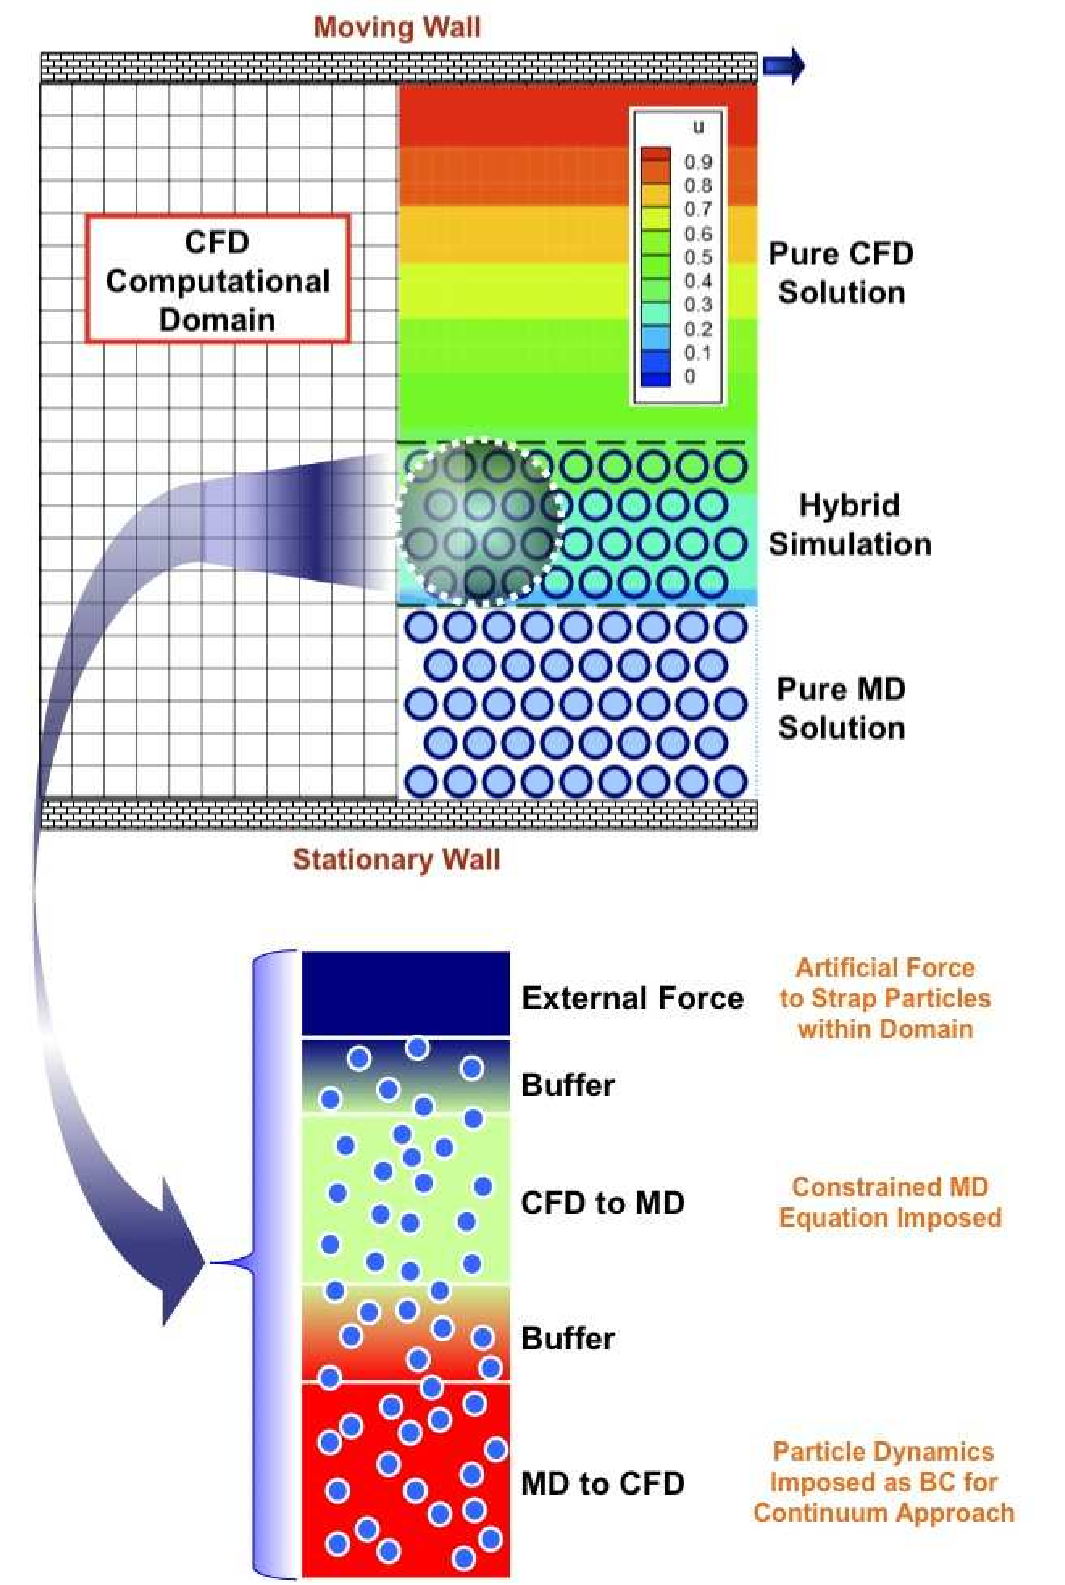
\includegraphics[scale=0.5]{fig1.pdf}
%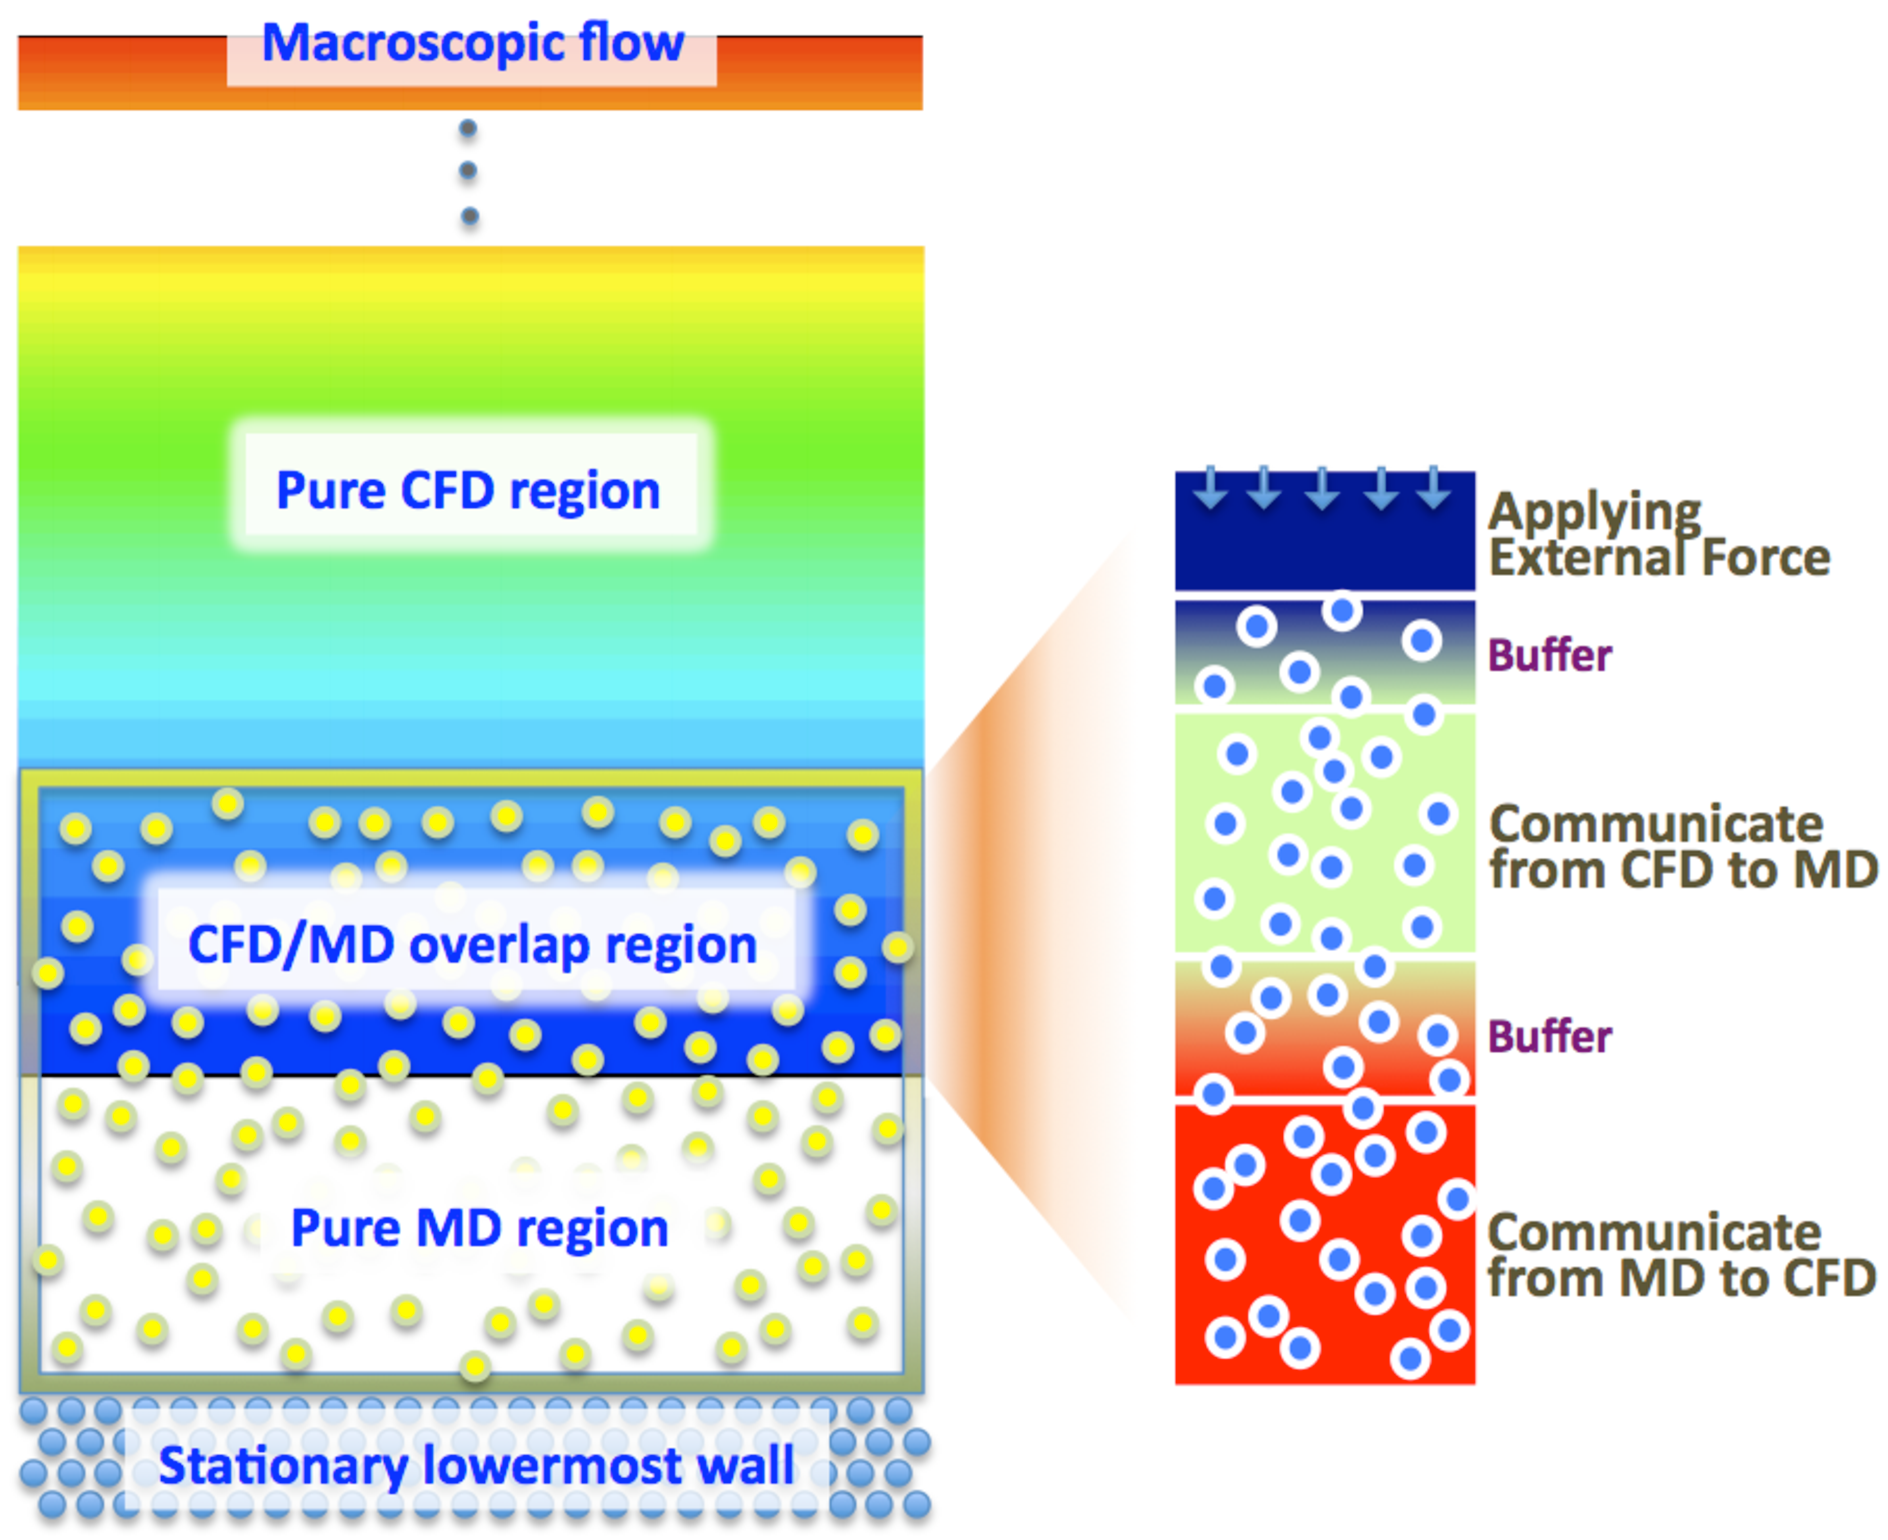
\includegraphics[scale=0.3]{Couette7.pdf}
%\linebreak
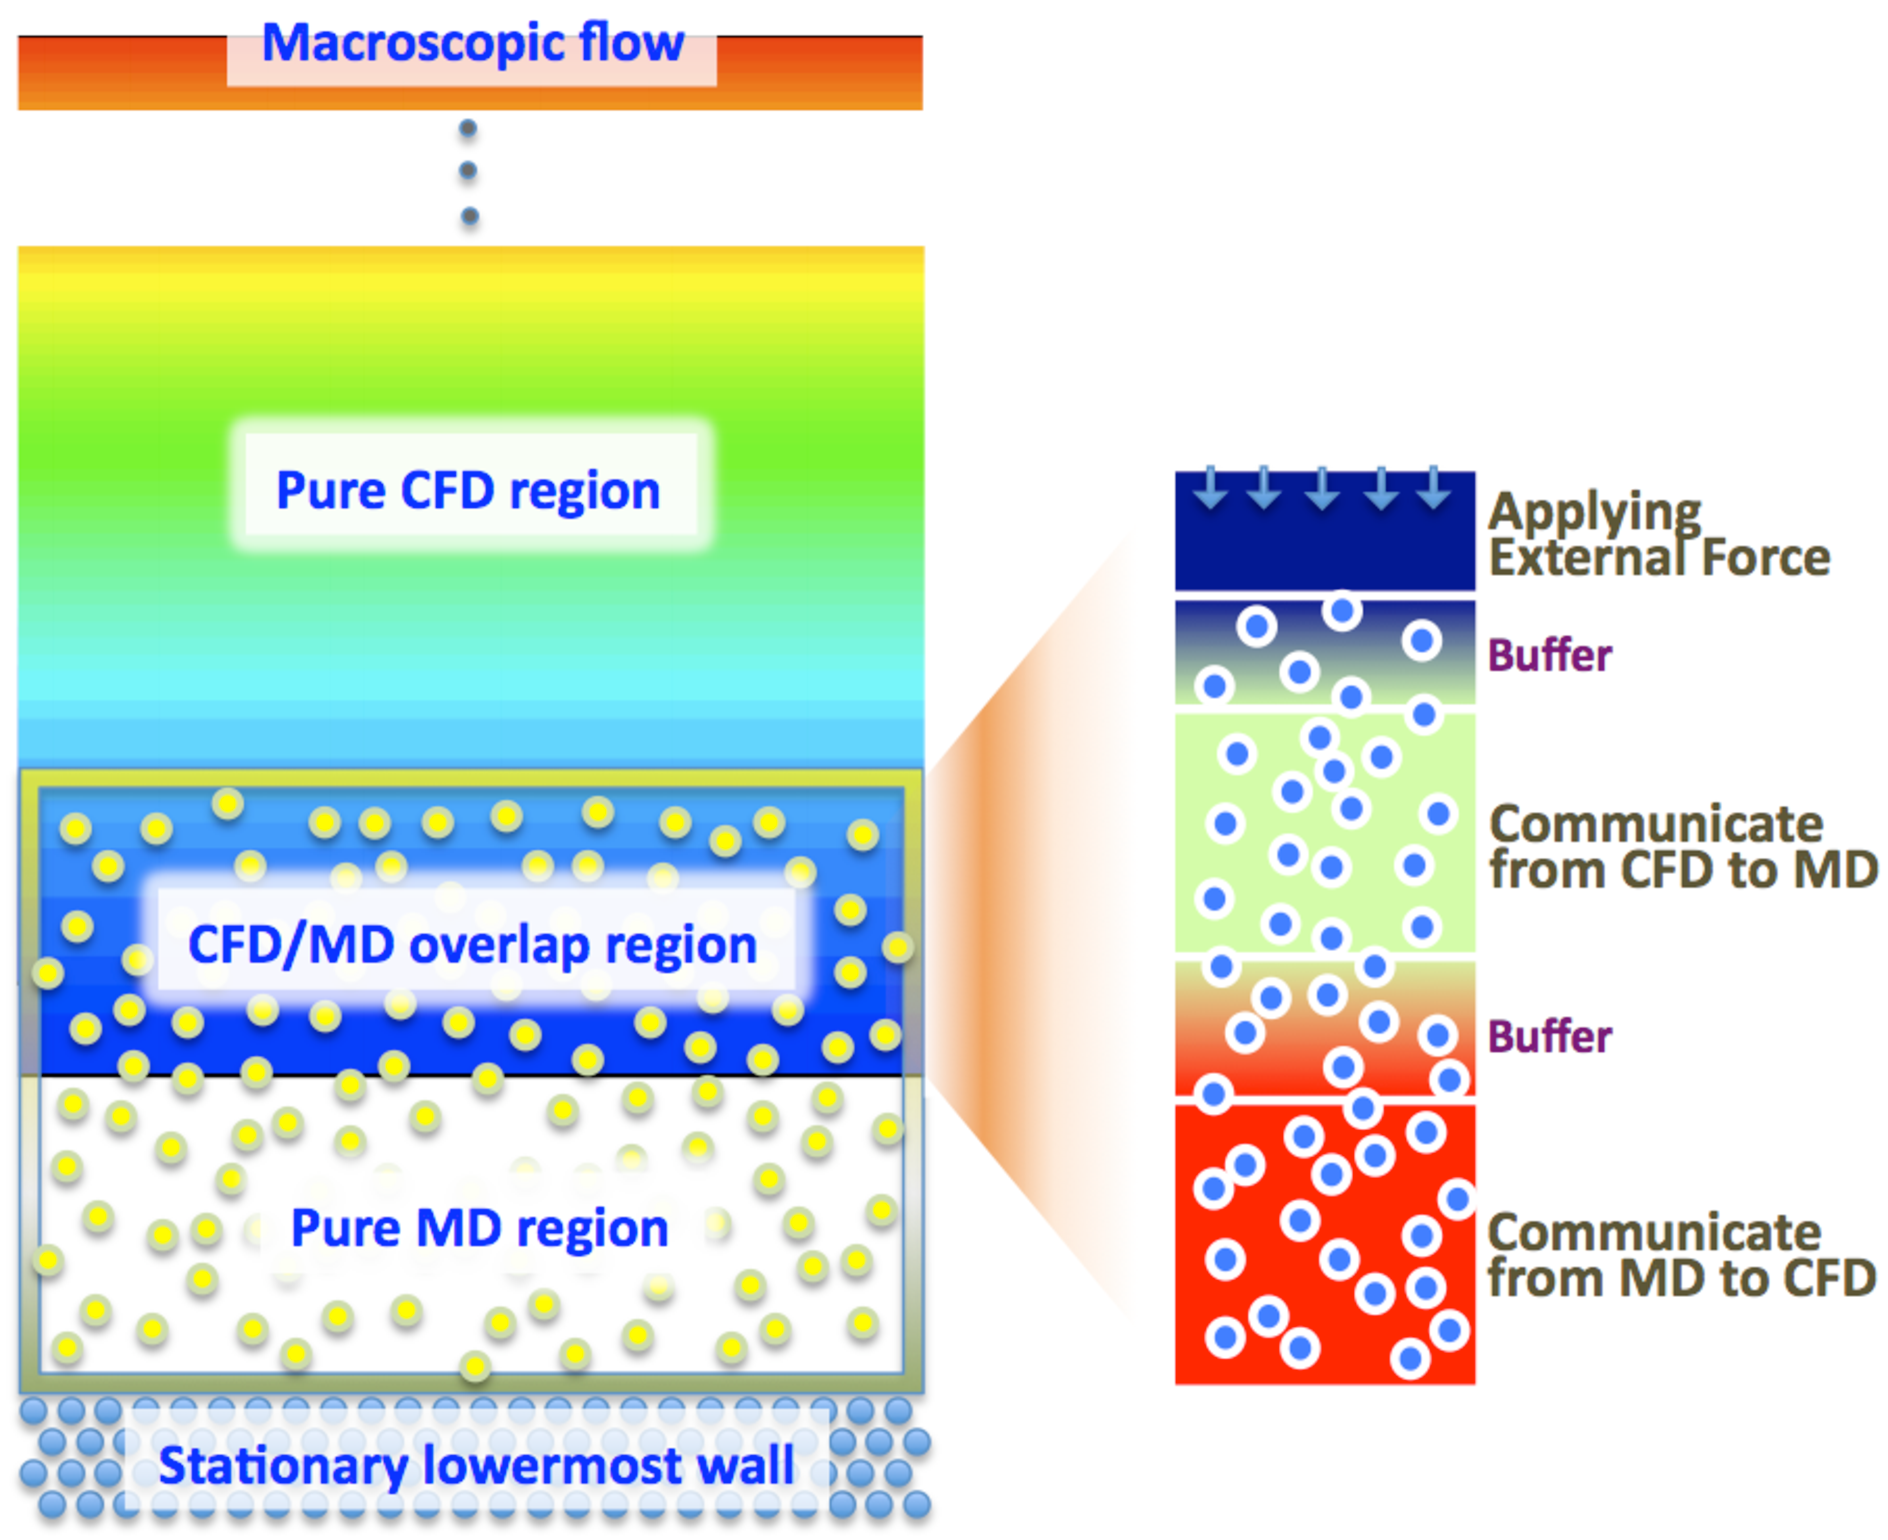
\includegraphics[width=0.8\linewidth]{Hybrid_Schematic.pdf}
%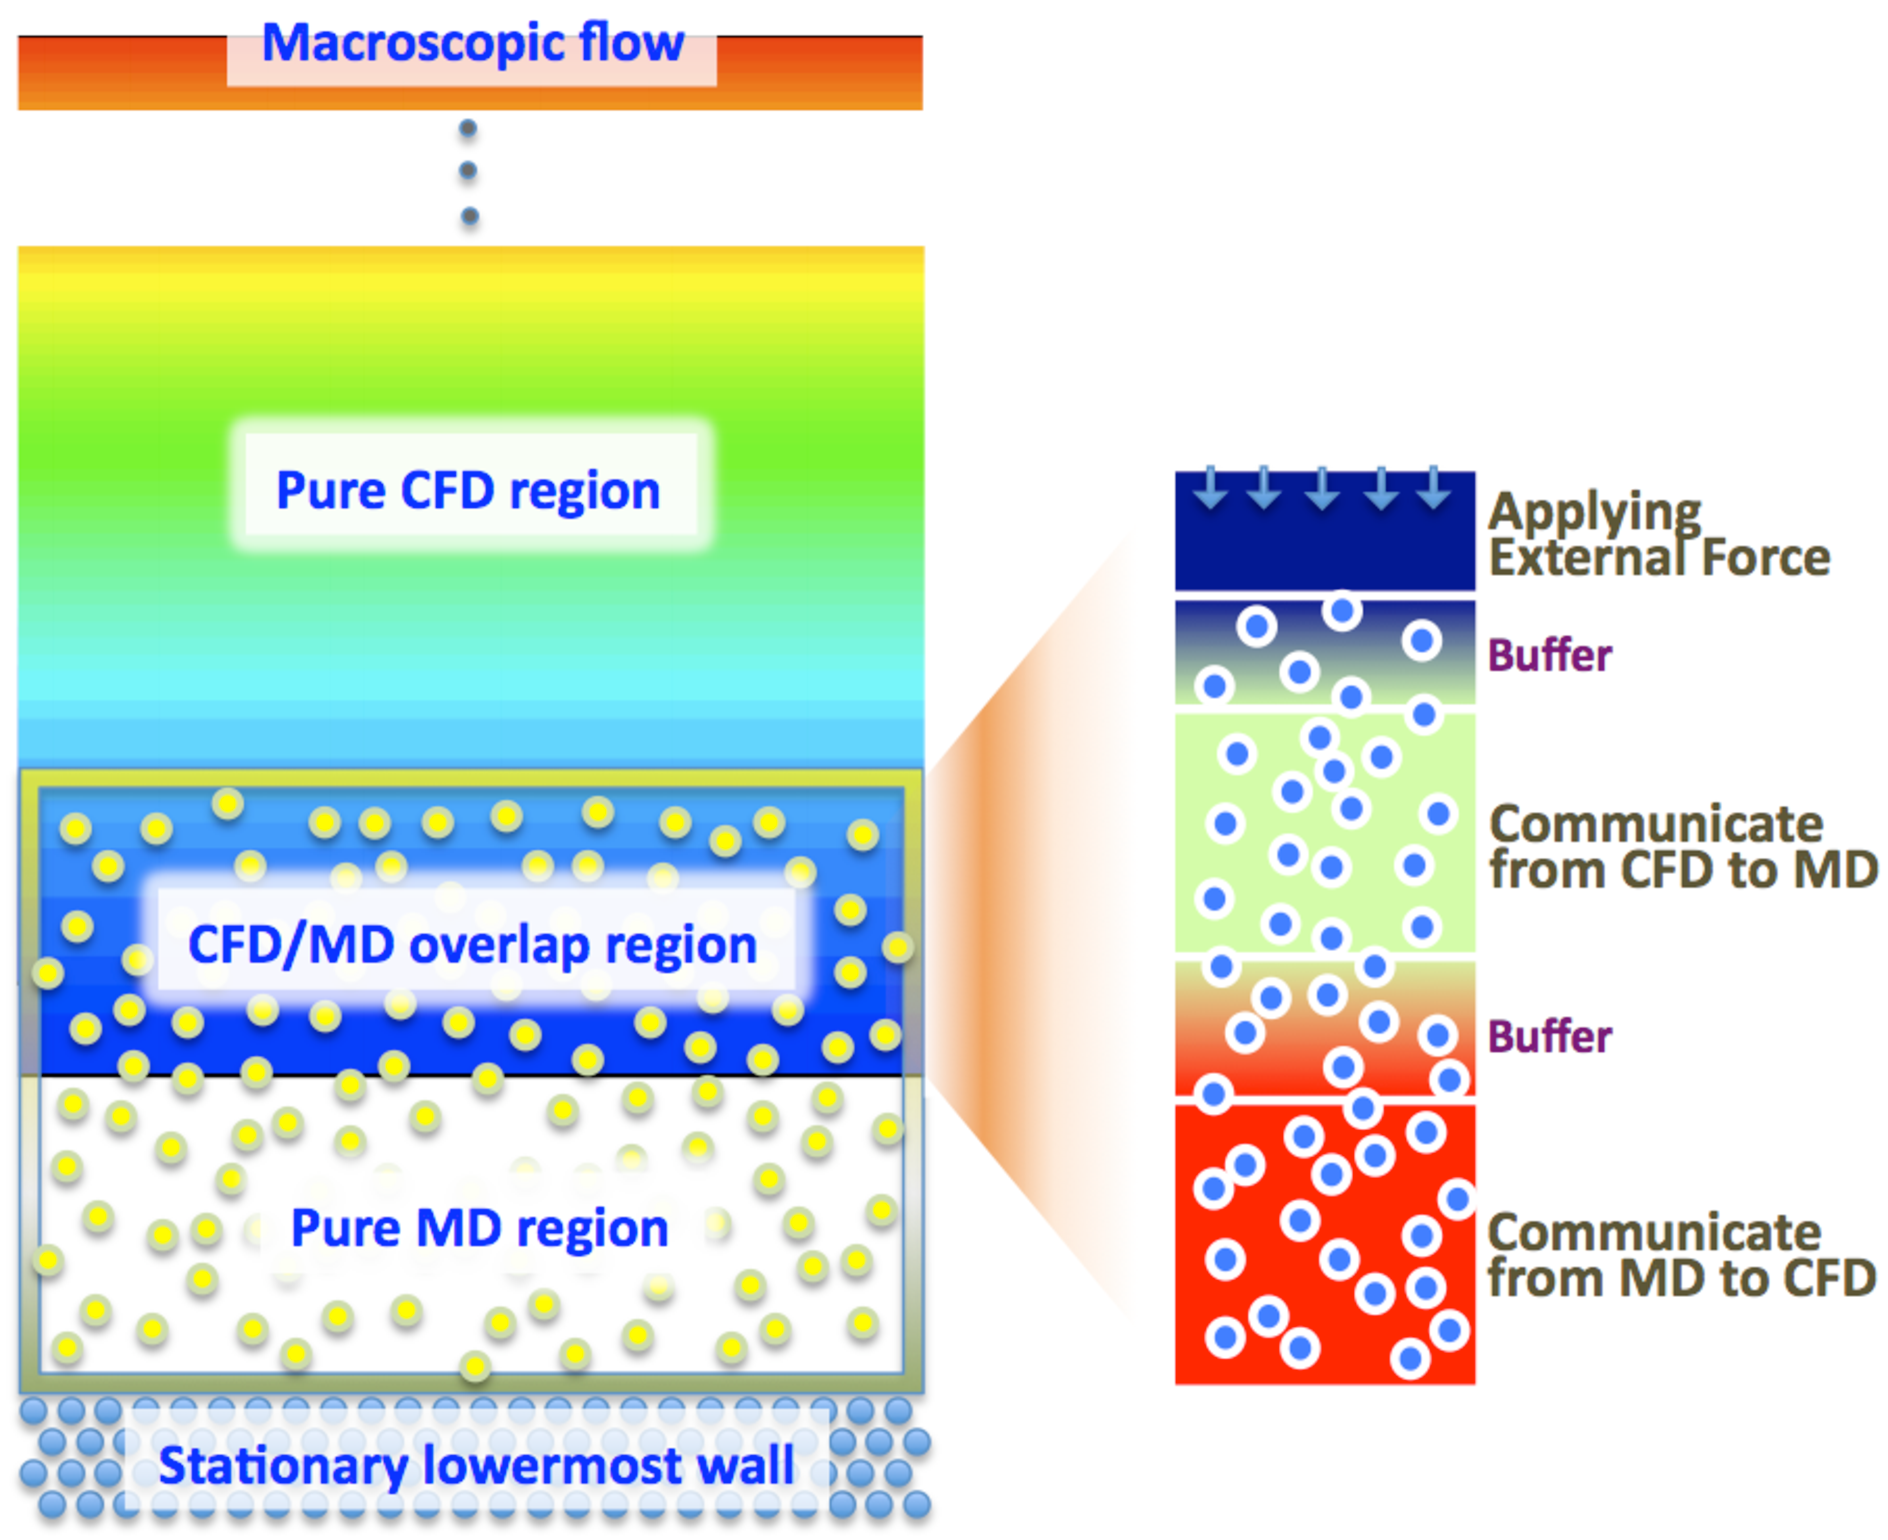
\includegraphics[width=1.0\linewidth]{Couette7.pdf}
\vskip-0.2cm
\caption{\small 
{\bf Schematic Diagram of the Hybrid Domain with Detailed View of Overlapping Zone}
; Overall continuum/atomistic and hybrid computational domain including overlap region is shown on lest figure. Detailed layer by layer explanation of overlapping region is indicated by right figure
%{\bf Schematic diagram of the hybrid domain.}
%Overall continuum/atomistic and hybrid computational domains for the chosen test problems (left) and a detailed view of the overlapping zone (right)
}
\label{Fig:Couette}
\vspace{-1em}
\end{figure}
%%%%% FIGURE %%%%%

This overlap region is designed sufficiently large to contain five individual layers of sufficient width for the purpose of their existence. The widths of these layers are of course problem dependent. Their roles in the hybrid region are as follows. One layer (the bottom one in Fig. 1-left) provides information from the particle (MD) domain to the continuum one (denoted as ''MDtoCFD''. A second layer (the third one from the bottom in Fig. 1-left) provides information from the continuum domain to the particle one (denoted as ''CFDtoMD''. A third layer (the top one in Fig. 1-left) applies a fictitious external force which prevents particles from escaping from the hybrid domain. These three ''active'' layers are separated by buffer layers, which are placed so as to ensure smooth transitions and that there is no direct correlation between the ''active'' layers. Properties (e.g. velocity) of particles spatially located in the MDtoCFD layer are ensemble-averaged over all the particles in the layer and also averaged over a finite time (''sampling duration''). The average value is communicated to the continuum solver periodically with a fixed period (''sampling interval'').

The height of each layer is the same as the CFD cell height and averaged conservative properties in two consecutive layers are passed to continuum domain to be directly imposed as the viscous boundary condition on the Navier-Stokes solver with collocated data structure. The CFDtoMD layer imposes the instantaneous values of properties, velocity in this case, resulting from the continuum solver. This is done via and appropriate constraint to the MD particle-based conservation of momentum on every single particle (constrained dynamics) in the CFDtoMD layer. Thus, particles in this layer are constrained to attain the macroscopic flow property (velocity in this case) on average, while preserving their degree-of-freedom of translational motion. In the uppermost layer, a fictitious external force is exerted on particles to prevent them from escaping the particle domain. This force function is designed to be short-range so as not to be strong enough to influence the motion of the particles past the buffer layer in the CFDtoMD domain. The force stiffens as the particles approach the location where the force becomes infinite in a way that minimizes reflections while preventing the particles from drifting out of the particle domain. The buffer layers existing in between each ''active'' layer are set up to be wider than the interaction length scale of the particles (cutoff radius), in order to prevent direct interaction between particles in neighboring ''active'' layers.
%\\}


%The hybrid simulation requires the implementation of hybrid interfaces and schemes on individual code. In the current study, the file interface is designed to schedule the information exchange between continuum and discrete particle descriptions.  A constrained Lagrangian dynamics model is implemented for hybrid simulation. Unit conversion routine is also implemented in the application code. These changes are summarized in table~\ref{table:interface_implementation}.

Hybrid simulation requires the implementation of hybrid interfaces and schemes based on an individual code. In the current study, the file interface is designed to schedule the information exchange between continuum and discrete particle descriptions. A constrained Lagrangian dynamics model is implemented for hybrid simulation. A unit conversion routine is also implemented in the application code. These changes are summarized in Table~\ref{table:interface_implementation}. 


% Table formats; h,t,b,p - here,top,bottom,page of floats
%\begin{table}[t]
\begin{table}
  \caption{\small
{\bf Implementation of hybrid interface on CFD and MD codes.} Both codes are equipped with the file-based information exchange routine, to update the hybrid boundary condition. CFD code experiences the global change of its data structure to store the information of the entire fluid system. MD code adopts 
hybrid equations to impose the macroscopic information on microscopic domain and to ensure numerical stability. 
}
  \label{table:interface_implementation}
  \centering
%  \resizebox{0.8\textwidth}{!} {
\footnotesize
 \begin{tabular}{>{\centering}p{0.15\textwidth} || p{0.3\textwidth} | p{0.3\textwidth} }
\hline
  & \centering CFD & \multicolumn{1}{c}{MD} \\
\hline
 Global Change & Overset Data Structure (\it{optional}) & \multicolumn{1}{c}{-} \\
\hline
 \centering External Force & \centering - & External Force Equation (Eqn.~\ref{eq:External_Force}) \\
\hline
% CFDtoMD &  - File Interface: Sender & {- File Interface: Receiver \\ - Constrained MD Equation (Eqn.~\ref{eq:Con3})} \\
 \multirow{2}{*}{CFDtoMD} &  \multirow{2}{*}{File Interface: Sender} & {File Interface: Receiver} \\
 & & Constrained MD Equation (Eqn.~\ref{eq:Con3}) \\
\hline
 MDtoCFD & File Interface: Receiver & File Interface: Sender \\
\hline
\end{tabular} %}
\vspace{-1em}
\end{table}


%The CFD code employs the data structure of overset mesh technique~\cite{Chimera} to ease the handling of coupling parameters. In other words, the entire fluid domain is generated as the CFD mesh system and pure MD region is turned off as the `Hole' cell in the terminology of overset technique. Likewise, MDtoCFD and CFDtoMD boundary cells are declared as `Fringe' and `Donor' cells, respectively. The labor of mesh regeneration according to the change of coupling parameters (position and depth of hybrid layers) disappears with the overset data structure.

The CFD code employs the data structure of the overset mesh technique~\cite{Chimera}  to ease the handling of the coupling parameters. In other words, the entire fluid domain is generated because the CFD mesh system and pure MD region is turned off as the ''hole'' cell in the terminology of the overset technique. Likewise, MD to CFD and CFD to MD boundary cells are declared ''fringe'' and ''donor'' cells, respectively. The labor of mesh regeneration due to the change in coupling parameters (the position and depth of the hybrid layers) disappears with the overset data structure.

%Both codes are equipped with the information exchange routine which consists of one file sender and one file receiver. These file interfaces are scheduled to turn on every sampling interval. The instantaneous properties in the Donor cells of continuum domain are transferred to MD site and referenced when applying constrained Lagrangian dynamics equation. Averaged molecular properties are sent to CFD domain and they are used as the boundary conditions of Fringe cells. All exchanged properties are written in MD unit: thus, CFD code is equipped with velocity unit conversion function and equation of state which changes the pressure solution from CFD site to equivalent density property in MD domain.

Both codes are equipped with the information exchange routine, which consists of one file sender and one file receiver. These file interfaces are scheduled to turn on every sampling interval. The instantaneous properties in the donor cells of the continuum domain are transferred to the MD site and referenced when the constrained Lagrangian dynamics equation is applied. The averaged molecular properties are sent to the CFD domain, and they are used as the boundary conditions of the fringe cells. All exchanged properties are written in the MD unit: thus, the CFD code is equipped with a velocity unit conversion function and an equation of state, which changes the pressure solution from the CFD site to the equivalent density property in the MD domain.

%Along with the file interface, additional equations of motion are employed on MD code to accurately describe the influence of macroscopic flow variation on particle domain. First, the external force should be imposed to prevent leaving particles from the control domain and the force is applied to the normal direction of uppermost MD layer. A cost-effective classical external force model by Nie {\it{et al.}}~\cite{Nie} is employed as,

In addition to the file interface, additional equations of motion are employed on the MD code to describe accurately the influence of macroscopic flow variation on the particle domain. First, external force should be imposed to prevent the particles from leaving the control domain; the force is applied in the normal direction of the uppermost MD layer. A cost-effective classical external force model by Nie {\it{et al.}}~\cite{Nie} is employed as

%\skonote{Or, shall we replace the last sentence to the follow? \\
%The design of external force is very important to exert the correct mean pressure on MD domain without local disturbance in the density field, as is expressed by Werder {\it{et al.}}~\cite{Werder}. Compared to other hybrid models, the external force design in constrained Lagrangian dynamics approach is less sensitive to the solution since particles in the buffer layer between external force layer and molecular dynamic boundary layer act as decreasing the influence of non-uniform density distribution. Thus, a cost-effective classical external force model by Nie {\it{et al.}}~\cite{Nie} looks still valid for acquiring the accurate solution.}

\vspace{-.2em}
%\footnotesize
\begin{equation}
 F_{ext, i} = -p_{a}\sigma\frac{y_{i}-Y_{n-1}}{1-(y_{i}-Y_{n-1})/(Y_{n}-Y_{n-1})}
 \label{eq:External_Force}
\end{equation}
\normalsize
%where $\it p_{a}$ denotes the average pressure in the MD region, $\it Y_{n}-Y_{n-1}$ is the thickness of the uppermost layer which is applied the force and $\it F_{ext}$ is the external force acting on $\it i^{th}$ particle located on position $\it y_{i}$.

where  $\it p_{a}$ denotes the average pressure in the MD region, $\it Y_{n}-Y_{n-1}$ is the thickness of the uppermost layer to which the force is applied, and $\it F_{ext}$ is the external force acting on ith particle located on position $\it y_{i}$.

%Next, on CFDtoMD layer, the macroscopic flow properties at specific time shall be introduced to lead the motion of multiple particles in that layer. To satisfy mass conservation, a certain number of particles are inserted into or removed from this layer according to the mass flux by CFD solution,

Next, at a specific time, the macroscopic flow properties are introduced on the CFD to MD layer to lead the motion of multiple particles in that layer. A very complicated numerical intervention is required to maintain the momentum conservation. The averaged velocity of particles in $\it J_{th}$ cell equals to the velocity $\it u_{J}$ in the continuum cell.
%mass To satisfy mass conservation, a certain number of particles is inserted into or removed from this layer according to the mass flux by the CFD solution,

%mass \vspace{-.2em}
%\footnotesize
%mass \begin{equation}
%mass n = -A \rho u_y \Delta t / m
%mass  \label{eq:Mass_Flux}
%mass \end{equation}
%mass \normalsize
%mass where $A$ is the horizontal area, $u_y$ is the vertical velocity component in the CFD solution and $\Delta t$ is the sampling interval.

%mass A very complicated numerical intervention is required to maintain the momentum conservation. The averaged velocity of particles in $\it J_{th}$ cell equals to the velocity $\it u_{J}$ in the continuum cell.

\vspace{-.2em}
%\footnotesize
\begin{equation}
 u_{J}(t) = \frac{1}{N_{J}} \displaystyle\sum_{i} v_{i}
 \label{eq:Con_vel}
\end{equation}
\normalsize
where $\it v_{i}$ is the velocity of $\it i^{th}$ particle and $\it N_{J}$ is the number of particles in the cell. The Lagrangian derivative of Eq.~\ref{eq:Con_vel} obtains,

\vspace{-.2em}
%\footnotesize
\begin{equation}
 \frac{Du_{J}(t)}{Dt} =  \displaystyle\sum_{i} \frac{\ddot{x_{i}}}{N_{J}}
 \label{eq:Lagrangian}
\end{equation}
\normalsize

The Classical MD equation of motion can be generalized to obtain the constraint by adopting the fluctuation in the acceleration of each particles, $\zeta_{i}$

\vspace{-.2em}
%\footnotesize
\begin{equation}
 \frac{F_{i}}{m_{i}} = \ddot{x_{i}}(t)  =   \frac{Du_{J}(t)}{Dt} + \zeta_{i} = \frac{\displaystyle\sum_{i}F_{i}(t)} {\displaystyle\sum_{i}m_{i}} +   \zeta_{i}
 \label{eq:Con2}
\end{equation}
\normalsize
where $\it F_{i}$ is the force on $\it i^{th}$ particle based on the interactions between particles,  $\it m_{i}$ is mass of each atom and  Eq.~\ref{eq:Con2} satisfies,
\vspace{-.2em}
%\footnotesize
\begin{equation}
\displaystyle\sum_{i}\zeta_{i}m_{i} = 0
 \label{eq:Con2}
\end{equation}
\normalsize

Finally, the constrained particle dynamics with the conventional equation of motion can be written as:

\vspace{-.2em}
%\footnotesize
\begin{equation}
 \ddot{x_{i}}(t) = \frac{F_{i}}{m_{i}} -  \frac{\displaystyle\sum_{i}F_{i}(t)} {\displaystyle\sum_{i}m_{i}} - \frac{1}{\Delta t_{MD}} \{  \frac{\displaystyle\sum_{i}m_{i}\dot{x_{i}}} {\displaystyle\sum_{i}m_{i}} - u_{J}(t + \Delta t_{MD})\}
 \label{eq:Con3}
\end{equation}
\normalsize

The continuum velocity and the mean microscopic velocity from MD over the control domain provide the synchronization of the mass and momentum consistent with Eqn.~\ref{eq:Con3}.




\subsection{Constrained Lagrangian Dynamics for Multi-species Flow Simulation}
\label{sec:hybrid_multispecies}

\skonote{To Nayong: What shall be added here}

1. How classical constrained Lagrangian dynamics equation is implemented

-- what is the objective: to eventually equilibrate the continuum and mean microscopic velocity

-- what is the governing equation: the governing equation and the meaning of each term under the equation

2. Why it needs change

-- The limitation of the equation to be applied to multi-species fluid model

3. How it is improved

-- The formulation of "Polyatomic Multi-species Constrained Lagrangian Dynamics Equation"

-- Difference compared to the original equation

-- Difference in applying the equation: apply on the center of mass of each molecule, not on individual atom (which will imply that atoms under the same molecule will experience the same acceleration, which tells that the linear momentum is of particular concern)

%%%%% End Hybrid Schema %%%%%


%%%%% Numerical Schemes %%%%%
\section{Development of a Hybrid CFD-MD Simulation Package}
\label{sec:numerics}

\subsection{Continuum Incompressible Flow Solver}
\label{sec:numerics_cfd}

%The current in-house continuum hydrodynamics code solves the unsteady incompressible Navier-Stokes equations to demonstrate the isothermal nano-scale flow field:
%\Nkimnote{
%\\=========== Modified version from ME ===========\\
The current in-house continuum hydrodynamics code solves the unsteady incompressible Navier-Stokes equations: 
%\\}

\vspace{-.2em}
%\vskip-.6cm
\begin{eqnarray}
\frac{\partial {u}_{i}}{\partial {x}_{i}} = 0
\end{eqnarray}
%\vspace{-.2em}
\vskip-.6cm
\begin{eqnarray}
\frac{\partial {u}_{i}}{\partial t} + \frac {\partial} {\partial {x}_{j}} ({u}_{i}{u}_{j}) = -\frac {\partial p} {\partial {x}_{i}} + \nu \frac {{\partial}^2 {u}_{i}} {{\partial} {x}_{j} \partial {x}_{j}} \nonumber
\end{eqnarray}
where $\nu$ is the kinematic viscosity.

%The primary difficulty in solving the incompressible Navier-Stokes equations in primitive variables stems from the lack of a time derivative in the continuity equation. There is no straightforward way to iteratively march these equations in time and ensure a divergence-free velocity field.

In this work, the pseudo-compressibility method~\cite{PseudoCompressibility} is adopted to form a hyperbolic system of equations which can be marched in pseudo-time.
%The method is extended to solve time-dependent problems by using sub-iterations in pseudo-time at each physical time step.
A time derivative of pressure is added to the continuity equation resulting in

%\vskip-.6cm
\vspace{-.2em}
\begin{eqnarray}
\frac{\partial (p/\rho)}{\partial \tau} = - \beta \frac{\partial {u}_{i}}{\partial {x}_{i}}
\end{eqnarray}
where $\beta$ denotes a pseudo-compressibility parameter, currently set up to 2.5.

For time-accurate unsteady simulation, a dual time stepping method is adopted and it is combined with the LU-SGS (Lower-Upper Symmetric Gauss-Seidel) scheme~\cite{LU-SGS} for the implicit time integration. The inviscid fluxes are upwind-differenced using Osher's flux-difference splitting scheme~\cite{Osher}. For higher-order spatial accuracy, the MUSCL (Monotone Upstream-centered Schemes for Conservation Laws)~\cite{MUSCL} approach is used on an inviscid flux calculation. Viscous fluxes are calculated using conventional second-order central differencing.


\subsection{Particle Dynamics Solver}
\label{sec:numerics_md}

%Molecular dynamics computer simulation technique is a specified computer simulation method for molecular systems, including microscopic details of a system and macroscopic statistical properties, which are the properties of the atoms, the interactions between particles, molecular characteristics, structure of molecules, transport phenomena etc.~\cite{Allen},\cite{Haile},\cite{Rapaport}

%Concise MD part -- Start
%In MD, an initial velocity is assigned to each atom, and Newton's laws are employed at the atomic level to propagate the system's motion through time evolution:

%\vspace{-.2em}
%\begin{equation}
%F_{i} = m_{i}a_{i}
%\label{eq:Newton}
%\end{equation}
%\normalsize
%here each atom $\it i $ in a system constituted by N atoms, mi is the mass of i$^{th}$ atom, ai is the acceleration and denoted by $\it {d^2r_{i}} / {dt^2}$, and $\it F_{i}$ is the force on i$^{th}$ atom, due to the atomic interaction which is calculated based on the potential energy between individual particles.

%The simplest choice for the potential energy $\it U(r)$  can be written as the sum of pairwise interactions of particles:

%\vspace{-.2em}
%\begin{equation}
%U(r_{1}, ...  ,r_{N}) =  \displaystyle\sum_{i} \displaystyle\sum_{j>i}  u(|r_{i} - r_{j}|)
%\label{eq:PEnergy}
%\end{equation}
%\normalsize
%where $\it i$ and $\it j$ particles are located at $r_{i}$ and $r_{j}$, and only $\it j>i$ cases have been considering for each particles pair once.

%The most commonly used two-body interaction model is the Lennard-Jones (12-6) potential is applied to calculate pairwise interaction and is define as:

%\vspace{-.2em}
%\begin{equation}
%u(|r_{i} - r_{j}|) = 4\epsilon_{ij}[(\frac{\sigma_{ij}}{r_{ij}})^{12}-(\frac{\sigma_{ij}}{r_{ij}})^{6}]
% \label{eq:LJ12}
%\end{equation}
%\normalsize
%where $\epsilon_{ij}$ and $\sigma_{ij}$ denote the pairwise potential well depth and the atom size parameter respectively, and $\it r_{ij}$ is the distance between the particle $\it i$ and $\it j$. The term $\it 1/r_{ij}^{12}$ dominating at short range distance repulsive behavior based on the Pauli principle to avoid overlapping the electronic clouds when particles are  brought very close to each other. The term $\it 1/r_{ij}^6$ dominates at long range attractive forces by van der Waals dispersion forces. The cut-off distance $\sigma_{c}$ is introduced here to reduce the computational cost and is set to be 2.2$\sigma$~\cite{Travis}.

%The time integration algorithm is required to integrate the equation of motion of the interacting particles and computing molecular trajectories, one of most common velocity Verlet algorithm is employed to compute the simulation.

%In this work,  the MD simulations were performed by using the modified version of Large Atomic Molecular Massively Parallel Simulator (LAMMPS). It is the classical molecular dynamics open-source code written in C++ and developed by Sandia National Labs.~\cite{LAMMPS_url}
%Concise MD part -- End

%In MD, an initial velocity is assigned to each atom, and Newton's laws are employed at the atomic level to propagate the system's motion through time evolution. To calculate pairwise interactions of particles in the system,  the most commonly used Lennard-Jones (12-6) potential interaction model is employed and is define as:
%\Nkimnote{
%\\=========== Modified version from ME ===========\\
In MD, an initial velocity is assigned to each atom, and Newton's conservation of momentum is employed at the atomic level to propagate the system's motion through time evolution. In this work the most commonly used Lennard-Jones (12-6) intermolecular force potential model is employed to calculate pair-wise interactions of particles in the system, and is defined as: 
%\\}
\vspace{-.2em}
%\footnotesize
\begin{equation}
 u(|r_{i} - r_{j}|) = 4\epsilon_{ij}[(\frac{\sigma_{ij}}{r_{ij}})^{12}-(\frac{\sigma_{ij}}{r_{ij}})^{6}]
 \label{eq:LJ12}
\end{equation}
\normalsize

%where $\epsilon_{ij}$ and $\sigma_{ij}$ denote the pairwise potential well depth and the atom size parameter respectively, and $\it r_{ij}$ is the distance between the particle $\it i$ and $\it j$. The term $\it 1/r_{ij}^{12}$ dominating at short range distance repulsive behavior based on the Pauli principle to avoid overlapping the electronic clouds when particles are  brought very close to each other. The term $\it 1/r_{ij}^6$ dominates at long range attractive forces by van der Waals dispersion forces. The cut-off distance $\sigma_{c}$ is introduced here to reduce the computational cost and is set to be 2.2$\sigma$~\cite{Travis}.

%The time integration algorithm is required to integrate the equation of motion of the interacting particles and computing molecular trajectories, one of most common velocity Verlet algorithm is employed to compute the simulation.

%In this work,  the MD simulations were performed by using the modified version of Large Atomic Molecular Massively Parallel Simulator (LAMMPS). It is the classical molecular dynamics open-source code written in C++ and developed by Sandia National Labs.~\cite{LAMMPS_url}

%\Nkimnote{
%\\=========== Modified version from ME ===========\\
where  $\epsilon_{ij}$ and $\sigma_{ij}$ denote the pair-wise potential well depth and the atom size parameter respectively, and rij is the distance between the particle i and j. The repulsive term $\it 1/r_{ij}^{12}$ dominating at short rij distance is based on the Pauli principle to avoid overlapping the electronic clouds when particles are very close to each other. The attractive term $\it 1/r_{ij}^{6}$ dominates at long range representing Van der Waals dispersion forces. A cut-off distance $\sigma_{c}$  is introduced here to reduce the computational cost and is set to be 2.2$\sigma$  [28]. Namely when rij exceeds the cutoff the intermolecular force is set to zero without being calculated.
The most common velocity Verlet algorithm is employed for time integration of the equations of motion of the interacting particles and to compute molecular trajectories in the simulation. 
In this work, the MD simulations were performed by using an appropriately modified version of the Large Atomic Molecular Massively Parallel Simulator (LAMMPS). It is a classical molecular dynamics open-source code written in C++ and developed by Sandia National Labs~\cite{LAMMPS_url}.
%\\}



\subsection{Incorporation of Hybrid Schemes}
\label{sec:numerics_hybrid}

Contents: how to design and setup domain - hybrid parameters; noise reduction - multiple replica sampling; how to exchange properties and match - exchanging interface + conversion of properties


One of the standard issues in obtaining coupled continuum to particle-based (MD) solutions is the fact that the particle-based (MD) solutions have noise, inherent because of limited size of particle ensemble averages and time-sampling limitations. This noise, if not kept under check, is passed on to the continuum solution yielding unphysical results. According to the mathematical expressions in statistical error~\cite{Hadjicon3,Time_Mechanism}, the ratio of sampling noise compared to the macroscopic velocity is inversely proportional to the square root of spatial layer size and temporal sampling duration. For example, reducing the macroscopic velocity by half requires either 4 times larger system domain or 4 times longer sampling to maintain the same order of accuracy. 

Sampling duration with interval, the size of sampling layer and its location are coupling parameters which define the scale and pattern of this noise. The layer size and sampling duration collectively work for reducing the noise, by increasing the number of particles participating in sampling process spatially and temporally. The layer size can be infinite along the periodic direction, while it is confined along the non-periodic direction to secure the sufficient space for pure CFD and MD domains. The sampling interval is denoted as the time increment between each information exchange. The frequent information exchange in the hybrid boundary zone is desired for the accuracy of the time-variant flow solution. This interval acts as the upper bound of sampling duration. The location of the sampling layer also influences the size of fluctuations. It has been noted that the sampling layer shall be placed sufficiently far from the solid obstacle to avoid the effect of strong interaction between fluid and solid particles~\cite{Nie,Yen}.

We reference to the determination of coupling parameters in previous studies~\cite{Nie,Yen,Liu,Hadjicon1,Hadjicon2,Werder,Flekkoy,Delgado1,Time_Mechanism} and intuitively design these parameters considering our application targets. We start from determining the location of the sampling layer according to other previous suggestions, e.g., at least 10$\sigma$ above the bottom wall in the nano-scale liquid argon system. The height of the sampling layer on the non-periodic direction is designed in a way that the sum of pure MD and hybrid regions does not exceed the half of the fluid system. For our deterministic transient/periodic applications, the sampling interval is roughly set to be within 1\% of the transition time or 10\% of the period. The sampling duration is designed the same as the sampling interval.

We also apply the replica sampling approach~\cite{REMD} to supplement the individual hybrid solution. Instead of changing coupling parameters for solving the same fluid system different flow conditions, we simulate the same coupling configuration with the variance in the initial Maxwell-Boltzmann distribution and average these replicas to find the non-fluctuating solution. In principle, the sampled solution from N replicas has the same order of accuracy as the individual solution from N times larger domain. The superiority of replica simulations over a single large-scale simulation can be found from the computational point of view: multiple moderate-sized jobs are more prone to get faster allocation than a single excessive resource requirement on most supercomputing batch queues. For the more, this approach is free from the geometric complexity so that it can be applied to the non-periodic three-dimensional flow simulations in which the virtual increase of sampling size is impossible.

%Molecular dynamics inherently describes the fluctuating pattern of particles, which becomes a noise in CFD solution. How to reduce this statistical error~\cite{Hadjicon3,Time_Mechanism} of averaged MD profile determines the accuracy of CFD solution.

%How to reduce the statistical error of averaged MD profile, which is the response of innate spatial/temporal locality in molecular dynamic systems, determines the accuracy of CFD solution in hybrid simulation. According to the mathematical expression in statistical error~\cite{Hadjicon3,Time_Mechanism}, the ratio of sampling noise compared to the macroscopic velocity is inversely proportional to the square root of spatial layer size and temporal sampling duration. For example, reducing the macroscopic velocity by half requires either 4 times larger system domain or 4 times longer sampling to maintain the same order of accuracy.

%2011 Reduction of the statistical error in the averaged MD profile, which is the response of innate spatial/temporal locality in molecular dynamic systems, determines the accuracy of the CFD solution in hybrid simulation. According to the mathematical expression in the statistical error ~\cite{Hadjicon3,Time_Mechanism}, the ratio of the sampling noise compared with the macroscopic velocity is inversely proportional to the square root of spatial layer size and temporal sampling duration. For example, in order to maintain the same order of accuracy, reducing the macroscopic velocity by half requires either a system domain that is four times larger or a sampling that is four times longer .

%\vspace{-.2em}
%\begin{eqnarray}
%E \propto \frac{1}{\sqrt{M}} \times \frac{1}{\sqrt{N}} \times \frac{1}{u_{\infty}}
 %\label{eq:noise}
%\end{eqnarray}
%where M is the number of independent samples, N is the number of particles spatially contained in that layer, and ${u_{\infty}}$ denotes the far field velocity.

% Eqn.~\ref{eq:noise} implies that the increase of system size or sampling duration is inevitable to solve the slower velocity field. Sampling duration is determined to be less than the sampling interval, which is chosen to be far smaller than the hydrodynamic characteristic time for time-accurate simulations. Since the hydrodynamic time scale is a function of characteristic size and kinematic viscosity, the sampling interval shall be fixed in solving the slower flow field. This, in turn, results in the impossibility to handle the sampling duration. Therefore, increasing the system size is the only possible way to maintain the same statistical accuracy, to be proportional to the square of the velocity change.


%Sampling duration with interval, the size of sampling layer and its position are coupling parameters which define the scale and pattern of this noise. The layer size and sampling duration collectively work for reducing the noise, by increasing the spatial and temporal sampling scales. Sampling interval is a factor which restricts the sampling duration. On unsteady simulations, a short sampling interval is preferred to frequently update temporal variation of flow field in hybrid boundary zones. This interval acts as the upper bound of sampling duration. The location of the sampling layer is a secondary factor which can locally increase the strength of fluctuation. Conventionally, sampling layer is placed far from the solid obstacle, e.g., at least 10 $\sigma$ above the bottom wall in solving the flow of the liquid argon~\cite{Yen}.

%2011 With regard to the sampling duration with intervals, the size of the sampling layer and its position are coupling parameters, which define the scale and pattern of this noise. The layer size and sampling duration collectively work to reduce the noise by increasing the spatial and temporal sampling scales. The sampling interval is a factor that restricts the sampling duration. In unsteady simulations, a short sampling interval is preferred to update frequently the temporal variation in the flow field in hybrid boundary zones. This interval acts as the upper bound of the sampling duration. The location of the sampling layer is a secondary factor that can increase the strength of fluctuation locally. Conventionally, the sampling layer is placed far from the solid obstacle, at least 10 $\sigma$ above the bottom wall to solve the flow of the liquid argon ~\cite{Yen}, for example.

%We introduce two numerical ideas to acquire the accurate hybrid solution. One is to quantitatively measure the scale of statistical noise in particular domain and the other is to numerically get the acceptable solution. The former shows the initial guideline to determine the coupling parameter and the latter refines the accuracy of the former solution.

%2011 We introduce two numerical ideas to acquire an accurate hybrid solution. One is to measure quantitatively the scale of statistical noise, the domain in particular, and the other is to obtain an acceptable solution numerically. The former shows the initial guideline to determine the coupling parameter and the latter refines the accuracy of the former solution.


%2011 \subsubsection{Determining Coupling Conditions}
%2011 \label{sec:numerical_parameters}
%The statistical noise is a function of the characteristics of fluid and surrounding solid elements, and geometric configurations, as well as the flow condition.
%Unfortunately, previous analyses on the strength of statistical error~\cite{Hadjicon3,Time_Mechanism} fail to consider the stronger interaction near the fluid-solid interface and the shape of the domain. We sense that the clear coupling parameters can be determined after the look-up of that specific system

%2011 The statistical noise is a function of the characteristics of the fluid, surrounding solid elements, and geometric configurations, as well as the flow condition. Unfortunately, previous analyses on the strength of the statistical error ~\cite{Hadjicon3,Time_Mechanism} failed to consider the stronger interaction near the fluid-solid interface and the shape of the domain. We sense that clear coupling parameters can be determined after the actual numerical simulation of that specific flow field.

%Our intuitive idea of numerically detecting the strength of statistical noise is to solve the stationary flow of the same fluid domain by pure MD method. The procedure is as follows.

%2011 Our intuition is that numerically detecting the strength of statistical noise solves the stationary flow of the same fluid domain by the MD method only. The procedure is as follows.

%2011 \begin{enumerate}
%2011 \item Empirical design of the sampling interval and the sampling layer's position\footnotemark
%2011 \item Structure construction\footnotemark
%2011 \item Simulation and collecting the temporal history of sampled velocity\footnotemark
%2011 \item Data processing\footnotemark
%2011 \item Determining the sampling layer size and the sampling duration\footnotemark$^{,}$\footnotemark
%2011 \end{enumerate}


%2011 \footnotetext[1]{The sampling interval is designed less than $1/100^{th}$ of hydrodynamic characteristic time; the location of the sampling layer is placed O(10) nanometers above the solid obstacle.}

%2011 \footnotetext[2]{The height of the domain can be reduced by placing a specular wall on the top, in case the system is sufficiently large; the length of the domain along the periodic direction can be arbitrarily chosen. The optimal length is further determined by the relation between the strength of noise and number of particles, i.e., $V_{noise}{\propto}1/\sqrt{N}$.}

%2011 \footnotetext[3]{Data collection starts as soon as the relaxation process is finished. The temporal history of averaged velocity from the smallest layer size with shortest sampling interval is stored.}

%2011 \footnotetext[4]{The dataset produced around the location of sampling layer is spatially and temporally averaged to produce the spatial and temporal variation of the sampled velocity.}

%2011 \footnotetext[5]{The noise is compared with the expected macroscopic velocity at that position, considering the linear velocity gradient from the wall to the far field. A paired condition which produces sufficiently small portion of noise and whose temporal duration is less than designed sampling interval is chosen to be the layer size and sampling duration of this hybrid simulation.}

%2011 \footnotetext[6]{If no condition is satisfactory, the acceptable condition can be obtained by either increasing the length of the computational domain based on $V_{noise}{\propto}1/\sqrt{N}$ or changing the position of the sampling layer and repeating data processing. The condition that generates the smallest MD domain in the hybrid simulation is chosen.}

%Change the position of sampling layer and conduct data processing again in case no condition is satisfactory. Or increase the length of computational domain to reduce the noise by $V_{noise}{\propto}1/\sqrt{N}$. There exists infinite number of coupling conditions which produce the same amount of statistical noise: the one which requires the smallest MD domain for hybrid simulation is chosen.

%2011 We argue that our idea is very easy to follow and computationally not expensive since the solution of the stationary flow is immediately collected.

%The sampling noise in the specific system is quantified by this stationary flow simulation.

%2011 This stationary flow simulation provides the amount of sampling noise in various sampling conditions.

%Meanwhile, this experiment does not provide the statistical error because predicting the macroscopic velocity is impossible except restricted number of flow systems whose analytic solutions are present.

%2011 Meanwhile, this experiment does not provide the accurate statistical error of the individual flow field because of the impossibility to predict the macroscopic velocity in the sampling layer.

%except some well-known flow systems. 

%2011 This necessitates us to investigate additional approach which is globally applicable.


%2011 \subsubsection{Sampling Multiple Independent Experiments}
%2011 \label{sec:numerical_lowspeed}

%So far, all hybrid CFD-MD applications have been restricted to extremely fast flow field of O(100) m/s velocity.
%The difficulty of solving moderate-speed flow field by a hybrid approach is explained as follows. The hydrodynamic time scale is expressed as a function of characteristic size and kinematic viscosity. This implies that the sampling interval is fixed regardless of the change in velocity. This, in turn, results in the impossibility to handle the sampling duration. Increasing the system size proportional to the square of the velocity change remains the only possible way to maintain the same statistical accuracy. Unfortunately, submitting excessively large-scaled simulation on public supercomputers unfavorably takes far long time to get allocated. In worse case, the simulation may exceed the capacity of the system. Thus, a different approach is necessary for efficiently simulating the low-speed flow field.

%2011 So far, all hybrid CFD-MD applications have been restricted to an extremely fast flow field of O(100) m/s velocity. The difficulty of solving a moderate-speed flow field by a hybrid approach is explained as follows. The hydrodynamic time scale is expressed as a function of characteristic size and kinematic viscosity, which implies that the sampling interval is fixed regardless of the change in velocity. This rigidity makes it impossible to handle the sampling duration. Increasing the system size proportional to the square of the velocity change remains the only possible way to maintain the same statistical accuracy. Unfortunately, submitting excessively large-scaled simulation on public supercomputers is unfavorable because allocation takes far too long. In the worse case, the simulation may exceed the capacity of the system. Thus, a different approach is necessary for efficiently simulating the low-speed flow field.

%Considering that the increase of the MD domain is technically bound by the computing capacity, a different approach is necessary for simulating the low-speed flow field.

%We propose sampling multiple independent hybrid simulations from a smaller domain instead of trying to run a single hybrid simulation in the large domain.
%For this purpose, we design a framework which samples multiple independent hybrid simulations.
%The initial velocity component at individual problem set is differently determined from a Maxwell-Boltzmann distribution and solutions from independent simulations are averaged to produce the final solution. The labour of manually administrating multiple job executions is resolved by using a BigJob framework, which is to be discussed in the Section~\ref{sec:computational}.

%2011 We propose sampling multiple independent hybrid simulations in a smaller domain instead of attempting to run a single hybrid simulation in a large domain. The initial velocity component in the individual datasets is determined differently from a Maxwell-Boltzmann distribution. Solutions for independent simulations are averaged to produce the final solution. The labor of manually administrating multiple job executions is resolved by using a BigJob framework, which is discussed in Section ~\ref{sec:computational}.

%Along with the advantage in computing capability, sampling multiple experiments provides another advantage of less-sensitivity to coupling conditions. Even if the coupling parameters are ill-chosen, highly noisy individual solution can be refined by the enough number of independent samples. This advantage also increases the value of capturing the magnitude of statistical noise in Section~\ref{sec:numerical_parameters}, because the requirement of predicting the macroscopic velocity in the sampled layer becomes less important.

%2011 In addition to advantage for computing capability, sampling multiple experiments provides the advantage of less sensitivity to coupling conditions. Even if the coupling parameters are ill chosen, a highly noisy individual solution can be refined by a sufficient number of independent samples. This advantage also increases the value of capturing the magnitude of the statistical noise as discussed in Section ~\ref{sec:numerical_parameters}, because the requirement of predicting the macroscopic velocity in the sampled layer becomes less important.
%Clear advantages of sampling multiple experiments are that the simulation is not bound by \textit{(1) computing capacity} and \textit{(2) flow characteristics} anymore.




%Two conventionally used coupling approaches of synchronized and sequential coupling strategies are depicted in Fig.~\ref{Hybrid_Timescale1}. In synchronized coupling, CFD and MD codes exchange the information in the overlapping region at each sampling interval (denoted by ${\Delta}t$) and independently evolve to the next exchange time step. In contrast, one domain advances to the next exchange time step and leads its counterpart to approach this point in sequential coupling. Comparing these two mechanisms, synchronized coupling clearly have a far better parallel efficiency compared to sequential coupling.~\cite{Time_Mechanism} Parallel performance in synchronized coupling can ideally reach the single code running in case an appropriate load-balancing between two domains is applied. Large overhead on waiting is inevitable in sequential way unless CFD and MD application components run in a single MPI communicator, which implies that two codes are unified. On the other hand, sequential approach is expected to produce more time-accurate solution because the boundary condition on following domain (CFD domain in the figure) is implicitly imposed.
%Time-lagging phenomenon in CFD boundary region is observed in both strategies, because averaged molecular dynamic properties over backward sampling duration (from $n{\Delta}t-{\Delta}t_{s}$ to $n{\Delta}t$) are used to impose the CFD boundary condition at that instance ($n{\Delta}t$). Thus, the extrapolation from previous MD solutions is necessary to eliminate the time-lagging by half of sampling duration (${\Delta}t_{S}/{2}$) in the CFD boundary zone.
%Two conventionally used coupling approaches of synchronized and sequential coupling strategies are depicted in Fig.~\ref{Hybrid_Timescale1}. In synchronized coupling, CFD and MD codes exchange the information in the overlapping region at each sampling interval (denoted by ${\Delta}t$) and independently evolve to the next exchange time step. In contrast, one domain advances to the next exchange time step and leads its counterpart to approach this point in sequential coupling. Comparing these two mechanisms, synchronized coupling has a far better parallel efficiency because both codes independently evolve to the next sampling interval, while sequential approach is expected to produce more time-accurate solution because the boundary condition on following domain (CFD domain in the figure) is implicitly imposed. Unfortunately, both strategies contain the time-lagging phenomenon in CFD boundary region, because averaged molecular dynamic properties over backward sampling duration (from $n{\Delta}t-{\Delta}t_{s}$ to $n{\Delta}t$) represents the CFD boundary condition at that instance ($n{\Delta}t$). Extrapolation from previous MD solutions is necessary to eliminate the time-lagging by half of sampling duration (${\Delta}t_{S}/{2}$) in the CFD boundary zone.

Two conventionally used coupling strategies (synchronized and sequential) are depicted in Fig.~\ref{Hybrid_Timescale1}. In synchronized coupling, CFD and MD codes exchange information in the overlapping region at each sampling interval (denoted by ${\Delta}t$) and independently evolve to the next exchange time step. In contrast, in sequential coupling, one domain advances to the next exchange time step and leads its counterpart to approach this point. Comparison of these two mechanisms shows that synchronized coupling has a far better parallel efficiency because both codes independently evolve to the next sampling interval, while the sequential approach is expected to produce a more time-accurate solution because the boundary condition of the following domain (the CFD domain shown in Fig.~\ref{Hybrid_Timescale1}) is implicitly imposed. Unfortunately, both strategies contain the time-lagging phenomenon in the CFD boundary region because molecular dynamic properties averaged over the backward sampling duration (from $n{\Delta}t-{\Delta}t_{s}$ to $n{\Delta}t$) represent the CFD boundary condition at that instance ($n{\Delta}t$). Extrapolation from previous MD solutions is necessary to eliminate the time lag to half that of the sampling duration (${\Delta}t_{S}/{2}$) in the CFD boundary zone.

%\begin{figure}[htbp]
\begin{figure}
\centering
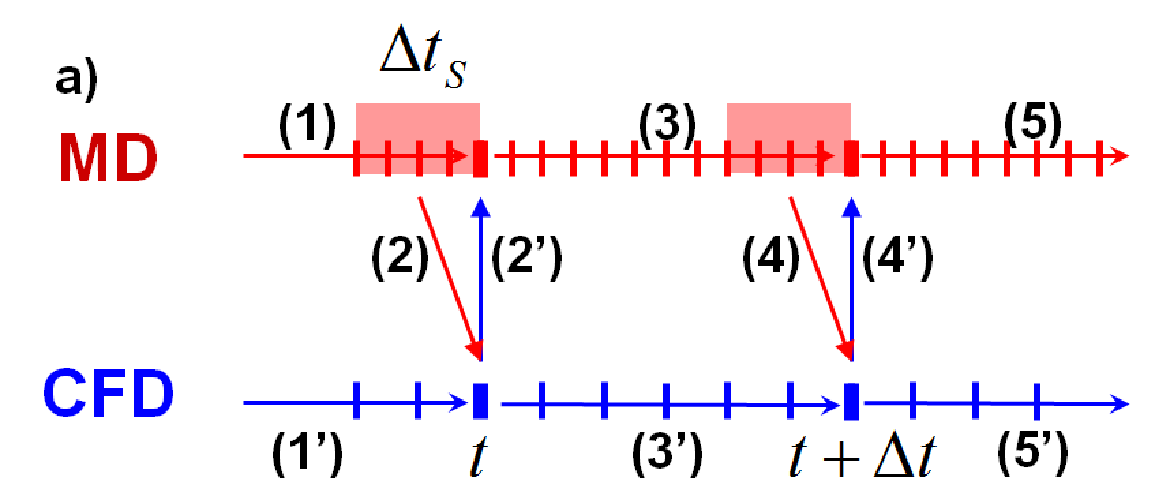
\includegraphics[width=0.8\linewidth]{Synchro_Coupling.pdf}
%\vskip-0.2cm
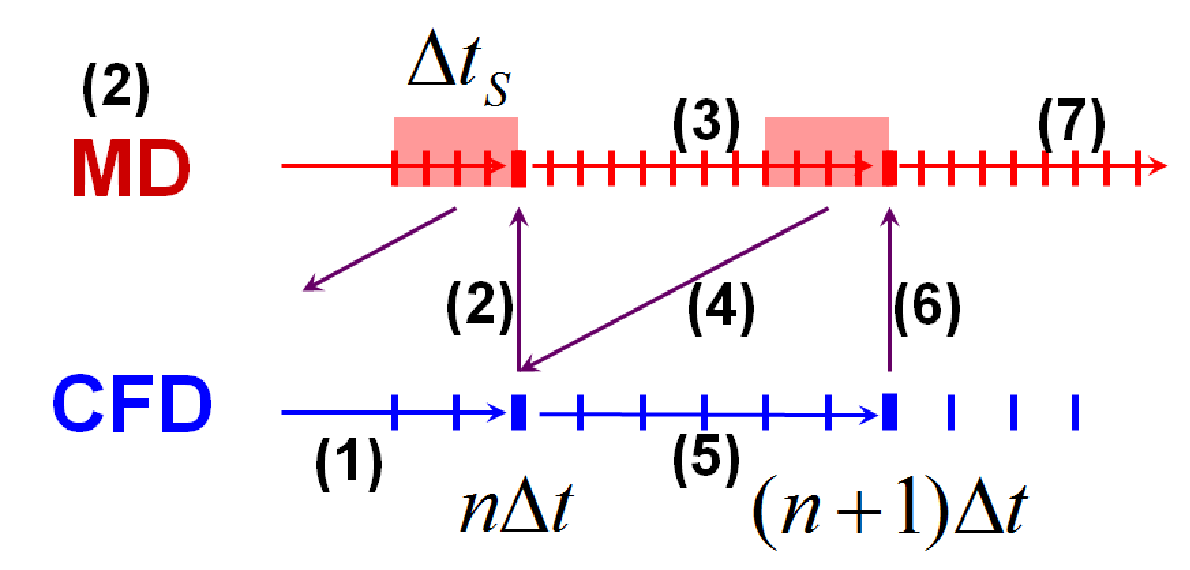
\includegraphics[width=0.8\linewidth]{Sequential_Coupling.pdf}
%\vskip-0.2cm
%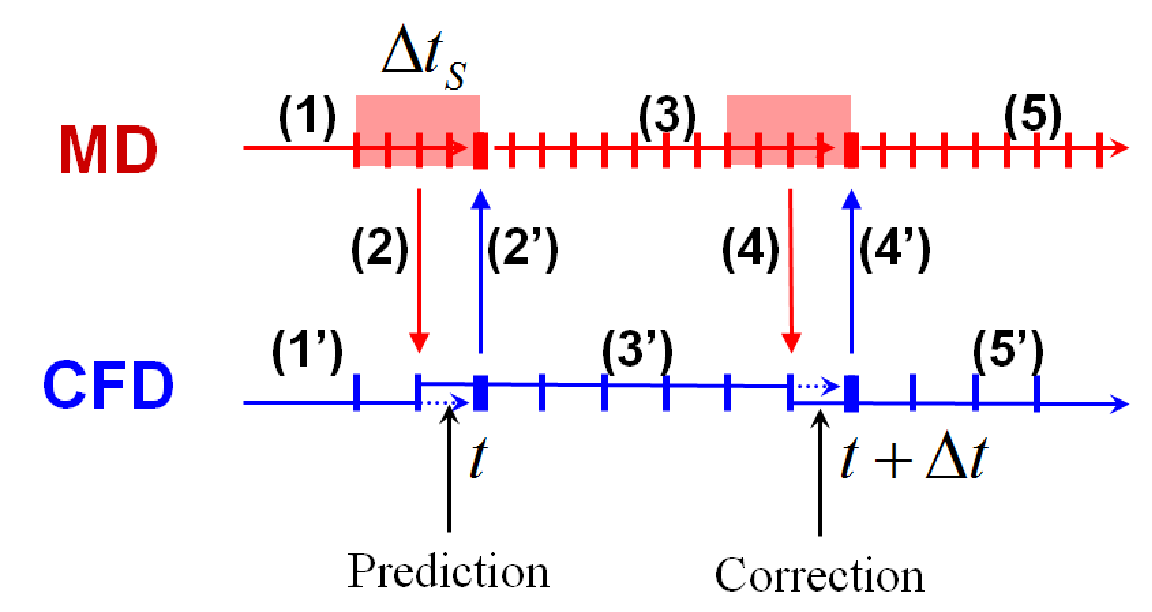
\includegraphics[width=1.0\linewidth]{Prediction_Correction_Coupling.pdf}
\vskip-0.2cm
\caption{\small {\bf Conventional time evolution mechanisms of a hybrid CFD-MD approach.} CFD and MD codes are scheduled to conduct data exchange in the overlapping region at every $\Delta{t}$ sampling interval. CFD solution at $n{\Delta}t$ is directly applied as the boundary condition for MD simulation and backward time-averaged molecular dynamic properties over $\Delta{t_{S}}$ sampling durations are imposed as CFD boundary conditions. (1) Synchronized Coupling: Both codes communicate at the same time level and independently iterate to next exchange point. (2) Sequential Coupling: From the same time level, one solver advances to the next communication point and impose implicit boundary condition to its counterpart.}
\label{Hybrid_Timescale1}
\end{figure}


%Time-lagging phenomenon in CFD boundary region is observed in both strategies, because averaged molecular dynamic properties over backward sampling duration (from $n{\Delta}t-{\Delta}t_{s}$ to $n{\Delta}t$) are used to impose the CFD boundary condition at that instance ($n{\Delta}t$). Thus, the extrapolation from previous MD solutions is necessary to eliminate the time-lagging by half of sampling duration (${\Delta}t_{S}/{2}$) in the CFD boundary zone which is accumulated at every sampling interval.
%As is presented in Fig.~\ref{Hybrid_Timescale2}-(0), Wang and He~\cite{Wang} proposed shifting the time axis of one domain by half of the sampling interval to eliminate this lagging effect. After both codes evolve by a sampling interval, the instantaneous CFD solution at $n{\Delta}t$ is communicated with averaged MD solution from $(n-1/2){\Delta}t$ to $(n+1/2){\Delta}t$. Two previous solutions from the counterpart are extrapolated to impose hybrid boundary conditions. The benefit of imposing extrapolated boundary condition is that the sampling duration can be designed as long as the sampling interval (${\Delta}t_{s}={\Delta}t$). However, the accuracy of extrapolated solution is worth to debate. In this scheduling, two \textit{previous} CFD solutions at $(n-1){\Delta}t$ and $n{\Delta}t$ are extrapolated to produce MD boundary conditions from $(n+1/2){\Delta}t$ to $(n+3/2){\Delta}t$. Except the velocity gradient is linear in time space, extrapolated properties fail to predict correct values throughout the simulation interval (from$(n+1/2){\Delta}t$ to $(n+3/2){\Delta}t$). The only way to reduce this extrapolation error is to reduce the sampling interval, which is contradictory to the condition for reducing the statistical error.

As is presented in Fig.~\ref{Hybrid_Timescale2}-(0), Wang and He~\cite{Wang} proposed shifting the time axis of one domain by half of the sampling interval to eliminate this lagging effect. After both codes evolve by a sampling interval, the instantaneous CFD solution at $n{\Delta}t$ is communicated with the averaged MD solution from from $(n-1/2){\Delta}t$ to $(n+1/2){\Delta}t$. Two previous solutions from the counterpart are extrapolated to impose hybrid boundary conditions. The benefit of imposing extrapolated boundary conditions is that the sampling duration can be designed to be as long as the sampling interval (${\Delta}t_{s}={\Delta}t$). However, the accuracy of the extrapolated solution is debatable. In this scheduling, two  \textit{previous} CFD solutions at $(n-1){\Delta}t$ and $n{\Delta}t$ are extrapolated to produce the MD boundary conditions from $(n+1/2){\Delta}t$ to $(n+3/2){\Delta}t$. Except when the velocity gradient is linear in time, the extrapolated properties fail to predict correct values throughout the simulation interval (from$(n+1/2){\Delta}t$ to $(n+3/2){\Delta}t$). The only way to reduce this extrapolation error is to reduce the sampling interval, which is contradictory to the condition for reducing the statistical error.

\begin{figure}
\centering
%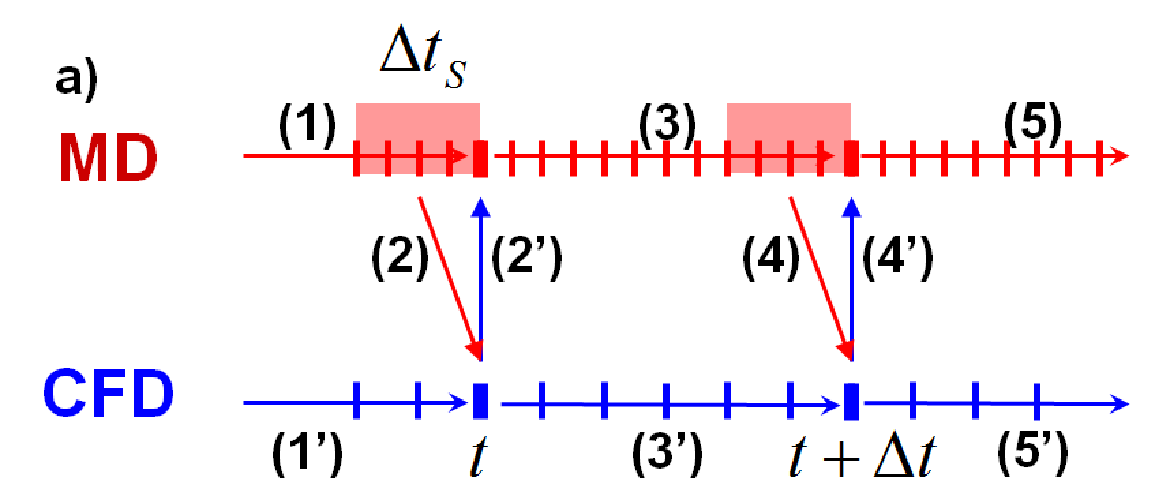
\includegraphics[width=1.0\linewidth]{Synchro_Coupling.pdf}
%\vskip-0.2cm
%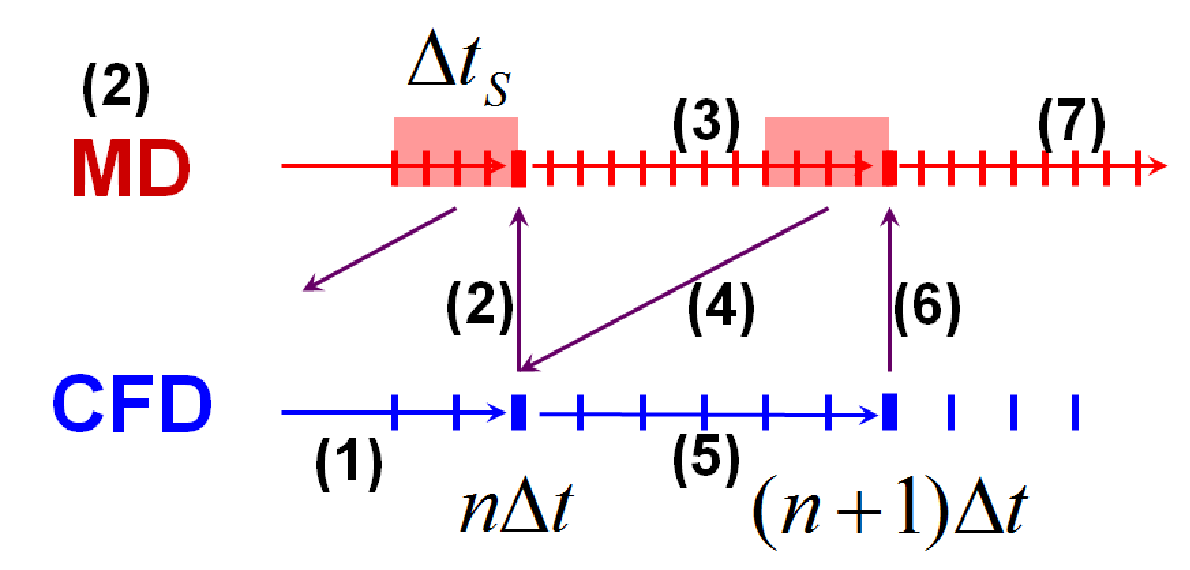
\includegraphics[width=1.0\linewidth]{Sequential_Coupling.pdf}
%\vskip-0.2cm
%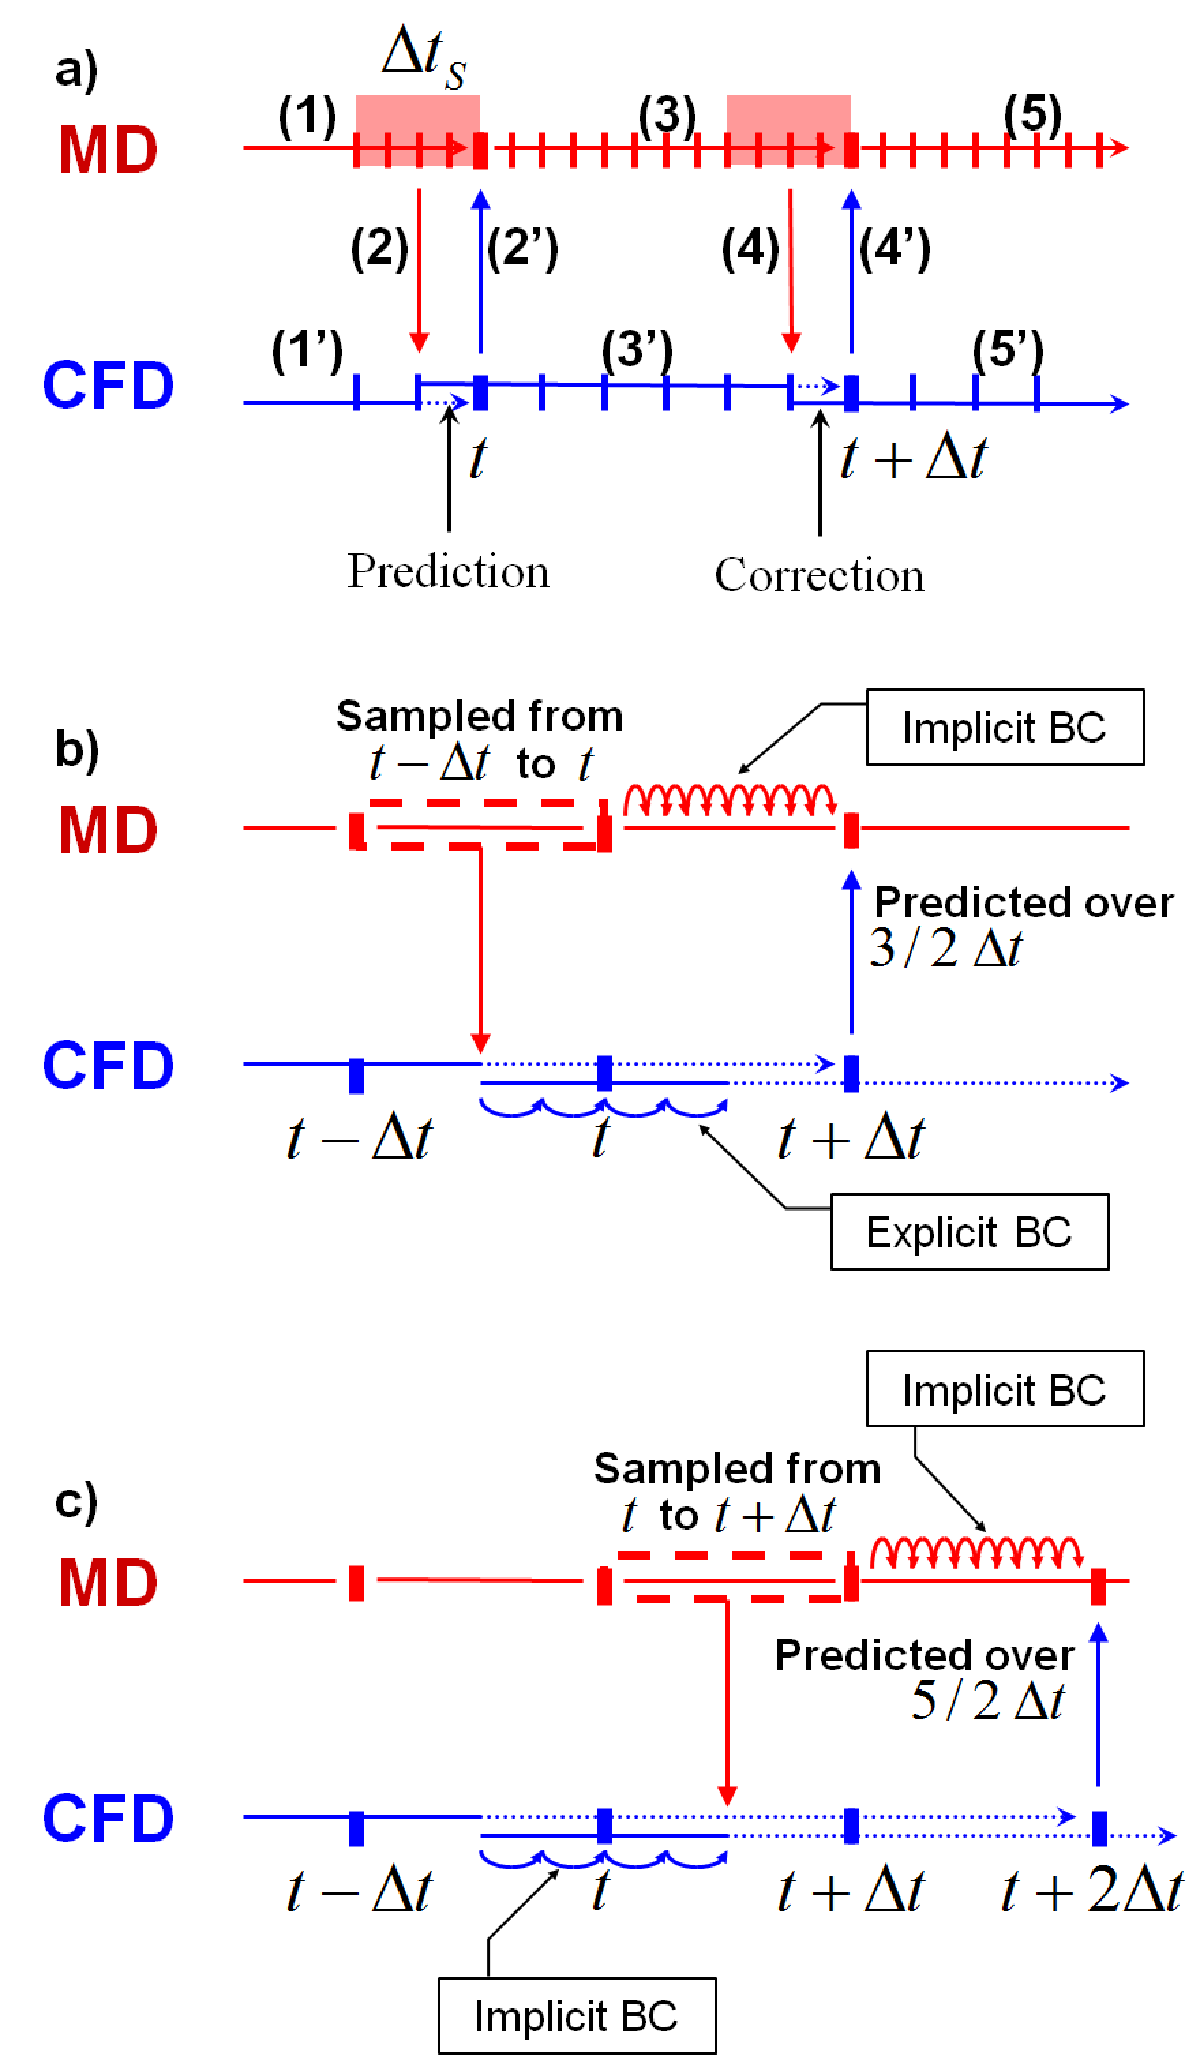
\includegraphics[width=0.6\linewidth]{Prediction_Correction_Full.pdf}
%\vskip-0.2cm
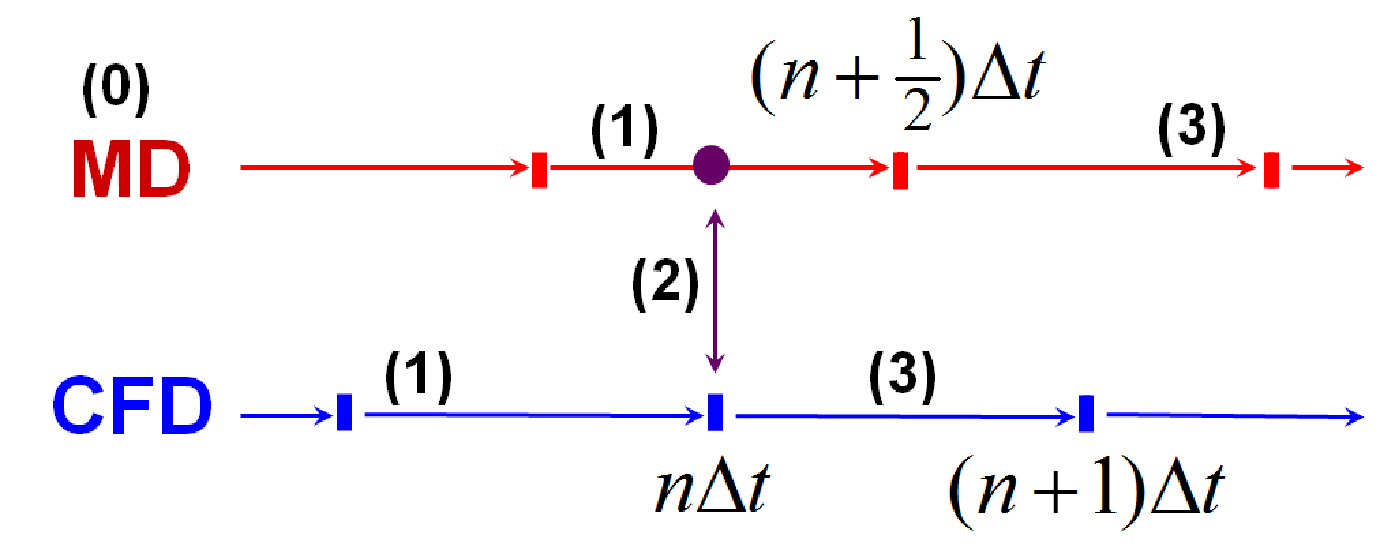
\includegraphics[width=0.7\linewidth]{Prediction_Correction_Org.pdf}
%\vskip-0.2cm
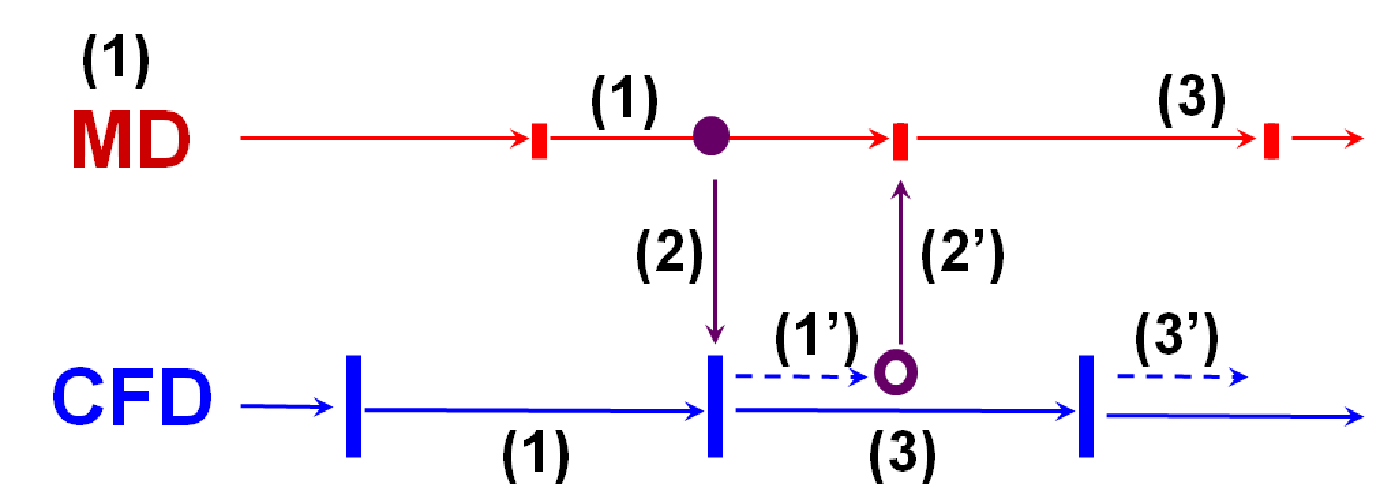
\includegraphics[width=0.7\linewidth]{Prediction_Correction_Extra_Simple.pdf}
%\vskip-0.2cm
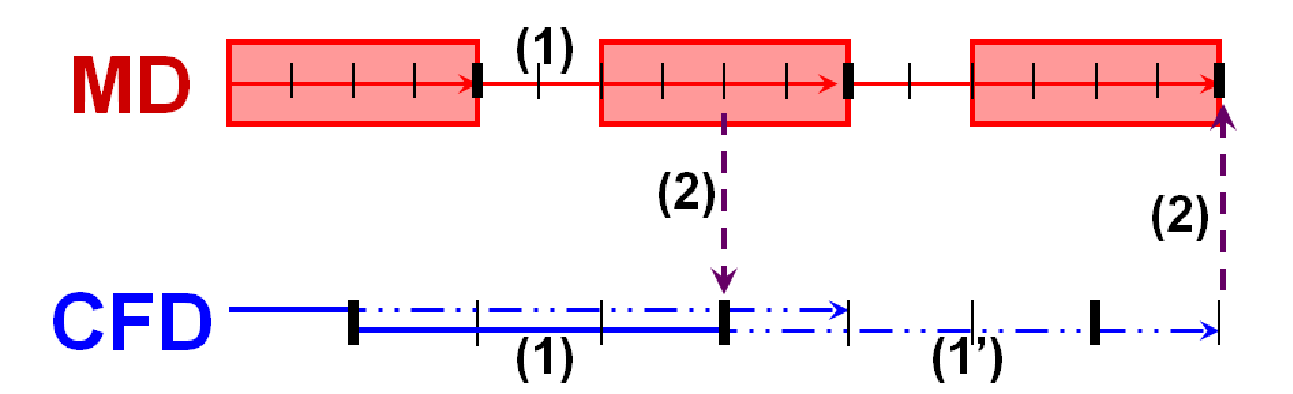
\includegraphics[width=0.7\linewidth]{Prediction_Correction_Inter_Simple.pdf}
%\vskip-0.2cm
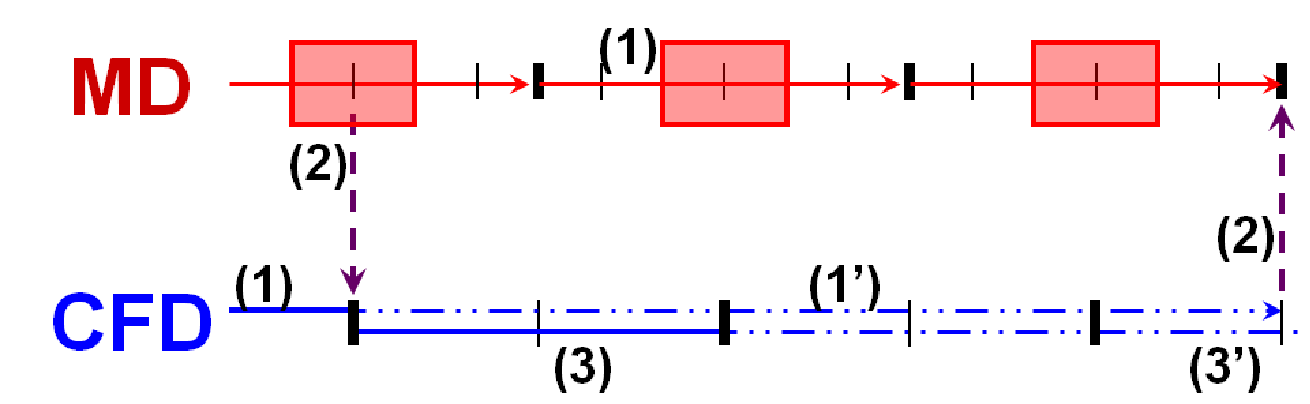
\includegraphics[width=0.7\linewidth]{Prediction_Correction_Both_Simple.pdf}
\caption{\small {\bf A prediction-correction approach with extrapolated / interpolated hybrid boundary conditions.} Applying extrapolation/interpolation enables increasing sampling duration as long as sampling interval. (0) Default Formulation;
%CFD code experiences extrapolated hybrid BC from the current MD solution, while MD code imposes the extrapolation from previous solutions by half of the sampling interval.
The hybrid BC in MD code is extrapolated from previous solutions.
% by half of the sampling interval.
(1) Extrapolated Boundary; CFD code runs the prediction step by $0.5{\Delta}t$. MD code imposes the hybrid BC by the extrapolation from the current value. (2) Interpolated MD Boundary; CFD code runs the prediction step by $1.5{\Delta}t$. MD code imposes interpolated hybrid BC. (3) Interpolated Hybrid Boundary Conditions; Time axis of CFD domain shifts back by 1 sampling interval and the prediction step is set $2.5{\Delta}t$. CFD and MD domains impose interpolated hybrid BC.}
\label{Hybrid_Timescale2}
\end{figure}


% The basic pattern of our approach is the same as the synchronized coupling. Main difference is, CFD code loads the previous solution at $t-{\Delta}t_{S}/{2}$ after communicating with MD code at $t$ and restarts the computation to the next communication point of $t+{\Delta}t$. Thus, time interval between $t - {\Delta}t_{S}/{2}$ and $t$ gets to be solved twice: first in prediction step and second in correction step. Clear benefit of current approach is that time-lagging problem is resolved without numerical treatments and additional computational overhead is acceptable because usually computational cost in MD simulation is dominant for a coupled simulation.
%A new scheme named ''prediction-correction approach'' is also depicted in Fig.~\ref{Hybrid_Timescale2}. The main difference from the default model is that CFD code iterates additional  time steps after the code evolved to the next data exchange time. For example, in Fig.~\ref{Hybrid_Timescale2}-(1), CFD code additionally evolves by the half of sampling interval after the code approached to $n{\Delta}t$. CFD code sends these predicted properties at $(n+1/2){\Delta}t$ to the MD site and receives averaged molecular properties around $n{\Delta}t$. CFD code loads its previous flow profile at $n{\Delta}t$ and runs the actual simulation to next communication point at $(n+1){\Delta}t$. Clear benefit of current approach is that both solvers extrapolate their boundary conditions from \textit{current} solutions (either exact solution or predicted values) instead of using \textit{previous} history. This eliminates the sensitivity of extrapolated solution according to the size of sampling interval in previous model, which enables increasing the sampling interval.

A new scheme named the ''prediction-correction approach'' is also depicted in Fig.~\ref{Hybrid_Timescale2}. The main difference from the default model is that the CFD code iterates additional time steps after it evolves to the next data exchange time. For example, in Fig.~\ref{Hybrid_Timescale2}-(1), the CFD code additionally evolves by half of sampling interval after it approaches $n{\Delta}t$. The CFD code sends these predicted properties at $(n+1/2){\Delta}t$ to the MD site and receives averaged molecular properties around $n{\Delta}t$. The CFD code loads its previous flow profile at $n{\Delta}t$ and runs the actual simulation to the next communication point at $(n+1){\Delta}t$. A clear benefit of the current approach is that both solvers extrapolate their boundary conditions from \textit{current} solutions (either exact solution or predicted values) instead of using \textit{previous} history. This advantage eliminates the sensitivity of the extrapolated solution to the size of the sampling interval in the previous model, which enables the increase of the sampling interval.

%This approach is further refined to increase the accuracy of the hybrid boundary condition by increasing prediction time scale. In Fig.~\ref{Hybrid_Timescale2}-(2), the prediction time scale is increased by one more sampling interval. While MD solver evolves for one sampling interval, CFD code iterates to the next communication point of MD time space. This enables MD boundary condition being interpolated by predicted CFD profiles. Figure ~\ref{Hybrid_Timescale2}-(3) demonstrates the imposition of interpolated boundary conditions on both domains. In this formulation, CFD time space is shifted backward by one sampling interval and prediction step is scheduled to be $(5/2){\Delta}t$.

This approach is further refined to increase the accuracy of the hybrid boundary condition by increasing the prediction time scale. In Fig.~\ref{Hybrid_Timescale2}-(2), the prediction time scale is increased by one more sampling intervals. While the MD solver evolves for one sampling interval, the CFD code iterates to the next communication point of MD time and space. This enables the interpolation of the MD boundary condition by the predicted CFD profiles. Figure ~\ref{Hybrid_Timescale2}-(3) demonstrates the imposition of interpolated boundary conditions on both domains. In this formulation, CFD time and space is shifted backward by one sampling interval and the prediction step is scheduled as $(5/2){\Delta}t$.


%A new approach named `prediction-correction strategy' is depicted in Fig.~\ref{Hybrid_Timescale2}. After the data exchange at $t$, MD advances to the next communication point by extrapolating two previous boundary conditions at $t-\Delta t$ and $t$. On the other hand, CFD code loads the previous solution at $t-{\Delta}t_{S}/{2}$ after communicating with MD code at $t$ and evolves to $t+{\Delta}t$ by imposing extrapolated boundary condition from data at $t-\Delta t - {\Delta}t_{S}/{2}$ and $t-{\Delta}t_{S}/{2}$, which makes the difference from the original strategy. In this approach, time interval between $t - {\Delta}t_{S}/{2}$ and $t$ gets to be solved twice: first in prediction step and second in correction step. Clear benefit of current approach is that both solvers are provided with the ``exact" boundary condition once in every sampling interval, compared to the original formulation in which boundary condition had to be extrapolated ``everytime" or the quasi-steady assumption had to be satisfied. As the exact boundary condition is provided at every sampling interval, sampling duration can be increased as long as sampling interval, which will reduce statistical error. Furthermore, with longer prediction setting as seen at Fig.~\ref{Hybrid_Timescale2}-b) and c), more accurate boundary condition can be imposed by simulating over longer prediction time.


The current numerical approach provides more accurate time-variant solution by decreasing or eliminating the unfavorable overshoot/undershoot phenomena in extrapolations. Nevertheless, an additional computational cost is inevitable for CFD simulation. We propose that the current approach to be used in the following conditions: (i) computational cost on CFD is quite smaller than that of MD, and (ii) the driving force that causes the flow variation is provided from the CFD domain. Without condition (i), the additional computational overhead for the prediction process will harm the performance of the simulation. If (ii) is not satisfied, the pattern of flow evolution cannot be predicted and the accuracy of the predicted solution is not guaranteed.





All applications we examine are internal flow fields filled with liquid argon. The characteristic length of liquid argon is ${\sigma}=3.405{\times}10^{-10}$ and the time scale is $\tau=2.2{\times}10^{-12}$. The density is $0.81m{\sigma}^{-3}$, which implies that 0.81 atoms are placed in the characteristic volume. The fluid domain is a channel system that consists of two virtically-placed parallel plates. The domain is filled with liquid argon particles and both walls have artificial properties that are the same as those of liquid argon. The slip ratio between fluid and solid particles is set at 0.6 to satisfy the linear velocity gradient along a vertical direction.~\cite{Nie}
%Channel height is set to In view of system size, two fluid systems are solved in our experiments, i.e., 10$^{-8}$ (52 $\sigma$) and 10$^{-7}$ (520 $\sigma$) meters in the height of channel. Applications covered in this work are periodic systems in the perpendicular direction and the flow variation is derived by the horizontal motion of an upper plate.
The channel is 52 $\sigma$ in height, which is O(10$^{-8}$) meters. Applications covered in this work are periodic systems in a perpendicular direction, and the flow is derived by the horizontal motion of the upper plate.


%As we proposed in Sec.~\ref{sec:numerical_noise}, we solve a stationary flow in the particle domain to determine coupling conditions. Table \ref{table:MD_Vel0} shows the averaged velocity depending on the layer size and sampling duration in the 10$^{-8}$ meter domain. Experiments were conducted with different lengths of the domain from 35 $\sigma$ to 70 and 140 $\sigma$. Noises at 0.2 non-dimensional height above the bottom wall are presented.
%% New
%We observe that increasing the length of the sampling layer is more effective in suppressing the sampling noise, compared to handling the sampling duration or the height of the sampling layer. However, increasing the length results in the increase of the molecular dynamic domain, which is unfavorable in view of computational cost. Thus, other two numerical treatments should be also considered.

%% Deleted
%The results of the individual test show that mathematical expressions on the strength of noise according to the height of the sampled layer and sampling duration~\cite{Hadjicon3,Time_Mechanism} do not coincide with our experiment. The first table shows that increasing the height of the averaged layer from 0.1 to 6.4 $\sigma$ reduces the statistical error by 4 times when the sampling duration is 1 $\tau$. This ratio worsens as the sampling duration increases. The same situation occurs in the sampling duration, which is contradictory to the previous mathematical expressions that were introduced in Sec.~\ref{sec:numerical_noise}. From the data analysis, we determined that the magnitude of the sampling noise depending on the layer size and sampling duration is far more complicated: $V_{N} = a \times SD^b \times LH^c \times SD^{d \times ln(LH)}$, where $V_N$ represents the velocity magnitude of the noise whose unit is $1/1000^{th}$ of the non-dimensional velocity, $SD$ denotes sampling duration and $LH$ is the height of the layer.
%%The mathematical expression on the strength of noise depending on the layer size and sampling duration is far more complicated than have been addressed in previous analyses: $V_{N} = a \times SD^b \times LH^c \times SD^{d \times ln(LH)}$, where $V_N$ represents the velocity magnitude of the noise, $SD$ denotes sampling duration and $LH$ is the height of the layer.
%% Deleted
%This equation is rewritten in simpler logarithmic formulation as

%% Deleted
%\vspace{-.2em}
%\footnotesize
%\begin{eqnarray}
%ln(V_{N}) = ln(a) +b~ ln(SD) +c~ ln(LH) +d~ ln(SD)~ ln(LH)\nonumber
%\label{eq:Noise1}
%\end{eqnarray}
%\normalsize
%% Deleted
%and these coefficients in our specific case are

%% Deleted
%\vspace{-.2em}
%\footnotesize
%\begin{eqnarray}
%&L = 35 \sigma :   &a = 33.67,~b= - 0.18,~c= - 0.30,~d=0.052\nonumber \\
%&L = 70 \sigma :   &a=25.85,~b=- 0.19,~c= - 0.27,~d=0.062\nonumber \\
%&L = 140 \sigma : &a=17.78,~b= - 0.18,~c=-0.25,~d=0.060\nonumber
%\label{eq:Noise2}
%\end{eqnarray}
%\normalsize
%% Deleted
%which directly expresses that 4 times longer sampling duration or 4 times larger layer height is far insufficient to half the noise.


%%\vspace{-.2em}
%%\footnotesize
%%\begin{eqnarray}
%%L = 35 \sigma :   ln(V_{N}) & = & ln(33.67) - 0.18~ ln(SD) - 0.30~ ln(LH) \nonumber \\
%%& + & 0.052~ ln(SD)~ ln(LH)\nonumber \\
%%L = 70 \sigma :   ln(V_{N}) &=& ln(25.85) - 0.19~ ln(SD) - 0.27~ ln(LH) \nonumber \\
%%&+& 0.062~ ln(SD)~ ln(LH) \\
%%L = 140 \sigma :   ln(V_{N}) &=& ln(17.78) - 0.18~ ln(SD) - 0.25~ ln(LH) \nonumber \\
%%&+& 0.060~ ln(SD)~ ln(LH)\nonumber
%%\label{eq:Noise}
%%\end{eqnarray}
%%\normalsize



%% Table formats; h,t,b,p - here,top,bottom,page of floats
%\begin{table}
%  \caption{\small {\bf Statistical error in the stationary flow simulation.} Pure MD simulations of 35 $\times$ 52, 70 $\times$ 52 and 140 $\times$ 52 ${\sigma}^2$ are conducted. Liquid is bound in Y-direction by upper and lower walls and able to move in X-direction where periodic boundary condition is imposed. Initial data up to 100 $\tau$ are disregarded to provide enough time for minimization. Velocity of particles around the central layer are accumulated over 512 $\tau$ by using {\it{fix-ave-spatial}} function in LAMMPS package and post-processed to get the average velocity at different layer size and sampling duration conditions. Statistical noise becomes about half at 4 times bigger domain. The unit is 1/1000 of non-dimensional MD velocity (1$\sigma$ / $\tau$).}
%  \label{table:MD_Vel0}
%  \centering
%%  \resizebox{0.8\textwidth}{!} {
%\footnotesize
%  \begin{tabular}{c || c c c c c c c}
%\hline
%	&	1 $\tau$	&	2 $\tau$	&	4 $\tau$	&	8 $\tau$	&	16 $\tau$	 &	32 $\tau$	&	64 $\tau$	\\
%\hline
%0.1 $\sigma$	&	62.332 	&	48.396 	&	40.245 	&	35.006 	&	26.761 	&	 21.605 	&	17.617 	\\
%0.2 $\sigma$	&	53.821 	&	43.877 	&	36.693 	&	32.067 	&	24.108 	&	 20.874 	&	18.912 	\\
%0.4 $\sigma$	&	46.200 	&	38.967 	&	33.122 	&	29.881 	&	24.044 	&	 19.666 	&	18.827 	\\
%0.8 $\sigma$	&	40.087 	&	35.490 	&	31.412 	&	28.671 	&	23.949 	&	 20.382 	&	19.255 	\\
%1.6 $\sigma$	&	32.455 	&	30.470 	&	27.382 	&	24.405 	&	20.140 	&	 17.494 	&	16.594 	\\
%3.2 $\sigma$	&	23.019 	&	21.877 	&	21.072 	&	18.534 	&	16.532 	&	 14.395 	&	13.643 	\\
%6.4 $\sigma$	&	16.113 	&	15.754 	&	15.289 	&	14.649 	&	13.459 	&	 12.909 	&	12.858 	\\
%%12.8 $\sigma$	&	13.293 	&	13.235 	&	13.065 	&	12.888 	&	12.668 	&	 12.622 	&	12.492 	\\
%\hline
%\hline
%	&	1 $\tau$	&	2 $\tau$	&	4 $\tau$	&	8 $\tau$	&	16 $\tau$	 &	32 $\tau$	&	64 $\tau$	\\
%\hline
%0.1 $\sigma$	&	44.207 	&	34.909 	&	28.885 	&	23.981 	&	17.466 	&	 12.986 	&	12.630 	\\
%0.2 $\sigma$	&	36.675 	&	31.260 	&	25.690 	&	22.203 	&	18.914 	&	 12.341 	&	11.695 	\\
%0.4 $\sigma$	&	32.370 	&	28.093 	&	24.062 	&	19.818 	&	17.875 	&	 12.819 	&	11.980 	\\
%0.8 $\sigma$	&	29.544 	&	26.477 	&	23.613 	&	19.966 	&	18.261 	&	 13.404 	&	12.521 	\\
%1.6 $\sigma$	&	24.729 	&	22.964 	&	21.099 	&	19.111 	&	17.878 	&	 14.058 	&	12.684 	\\
%3.2 $\sigma$	&	18.719 	&	18.102 	&	17.111 	&	16.487 	&	15.723 	&	 13.074 	&	12.115 	\\
%6.4 $\sigma$	&	12.791 	&	12.596 	&	12.388 	&	12.121 	&	11.723 	&	 10.311 	&	9.536 	\\
%%12.8 $\sigma$	&	7.764 	&	7.687 	&	7.560 	&	7.425 	&	7.157 	&	 6.864 	&	6.565 	\\
%\hline
%\hline			
%	&	1 $\tau$	&	2 $\tau$	&	4 $\tau$	&	8 $\tau$	&	16 $\tau$	 &	32 $\tau$	&	64 $\tau$	\\
%\hline
%0.1 $\sigma$	&	30.578 	&	24.249 	&	19.228 	&	15.659 	&	13.238 	&	 10.163 	&	9.308 	\\
%0.2 $\sigma$	&	26.803 	&	21.931 	&	18.138 	&	14.721 	&	11.844 	&	 10.045 	&	8.494 	\\
%0.4 $\sigma$	&	23.158 	&	19.426 	&	16.965 	&	13.620 	&	10.759 	&	 9.742 	&	8.355 	\\
%0.8 $\sigma$	&	20.055 	&	17.501 	&	15.703 	&	13.378 	&	10.527 	&	 9.796 	&	8.069 	\\
%1.6 $\sigma$	&	15.966 	&	14.691 	&	13.486 	&	11.888 	&	9.944 	&	 9.398 	&	8.034 	\\
%3.2 $\sigma$	&	12.584 	&	12.144 	&	11.623 	&	10.484 	&	9.755 	&	 9.295 	&	8.376 	\\
%6.4 $\sigma$	&	10.243 	&	10.091 	&	9.860 	&	9.662 	&	9.189 	&	 9.059 	&	8.117 	\\
%%12.8 $\sigma$	&	7.832 	&	7.795 	&	7.722 	&	7.639 	&	7.515 	&	 7.471 	&	6.634 	\\
%\hline
%%\hline
%%L=280	&	1 $\tau$	&	2 $\tau$	&	4 $\tau$	&	8 $\tau$	&	16 $\tau$	&	32 $\tau$	&	64 $\tau$	\\
%%\hline
%%0.1 $\sigma$	&	21.947 	&	17.943 	&	14.922 	&	13.514 	&	11.377 	&	 7.454 	&	5.684 	\\
%%0.2 $\sigma$	&	19.120 	&	16.316 	&	14.028 	&	12.897 	&	10.611 	&	 7.053 	&	5.606 	\\
%%0.4 $\sigma$	&	16.985 	&	14.727 	&	12.997 	&	11.137 	&	9.159 	&	 5.999 	&	5.342 	\\
%%0.8 $\sigma$	&	14.825 	&	13.211 	&	11.920 	&	10.297 	&	8.840 	&	 5.792 	&	5.049 	\\
%%1.6 $\sigma$	&	11.517 	&	10.525 	&	9.714 	&	8.487 	&	7.479 	&	 5.230 	&	4.663 	\\
%%3.2 $\sigma$	&	7.900 	&	7.549 	&	7.082 	&	6.498 	&	5.857 	&	 4.772 	&	4.470 	\\
%%6.4 $\sigma$	&	5.383 	&	5.269 	&	5.132 	&	4.764 	&	4.488 	&	 3.598 	&	3.472 	\\
%%12.8 $\sigma$	&	3.601 	&	3.557 	&	3.514 	&	3.347 	&	3.256 	&	 3.017 	&	2.909 	\\
%%\hline
%%\hline
%%L=35,Vtot	&	1 $\tau$	&	2 $\tau$	&	4 $\tau$	&	8 $\tau$	&	 16 $\tau$	&	32 $\tau$	&	64 $\tau$	\\
%%\hline
%%0.1 $\sigma$	&	61.791 	&	48.230 	&	35.128 	&	27.260 	&	21.945 	&	 20.630 	&	17.077 	\\
%%0.2 $\sigma$	&	54.494 	&	44.894 	&	35.304 	&	28.244 	&	24.517 	&	 22.413 	&	20.046 	\\
%%0.4 $\sigma$	&	46.704 	&	39.673 	&	32.427 	&	27.454 	&	24.745 	&	 23.169 	&	21.168 	\\
%%0.8 $\sigma$	&	38.843 	&	34.431 	&	29.961 	&	25.884 	&	23.436 	&	 22.492 	&	20.849 	\\
%%1.6 $\sigma$	&	32.594 	&	30.621 	&	27.078 	&	24.190 	&	21.541 	&	 21.007 	&	20.151 	\\
%%3.2 $\sigma$	&	25.387 	&	24.468 	&	23.165 	&	21.798 	&	20.246 	&	 19.848 	&	19.701 	\\
%%6.4 $\sigma$	&	21.367 	&	21.131 	&	20.858 	&	20.374 	&	18.953 	&	 18.704 	&	18.701 	\\
%%12.8 $\sigma$	&	17.141 	&	17.047 	&	16.917 	&	16.700 	&	16.388 	&	 16.381 	&	16.380 	\\
%%\hline
%%\hline
%%L=70,Vtot	&	1 $\tau$	&	2 $\tau$	&	4 $\tau$	&	8 $\tau$	&	 16 $\tau$	&	32 $\tau$	&	64 $\tau$	\\
%%\hline
%%0.1 $\sigma$	&	44.319 	&	35.102 	&	29.449 	&	25.868 	&	21.739 	&	 15.653 	&	13.795 	\\
%%0.2 $\sigma$	&	38.577 	&	32.558 	&	27.460 	&	23.998 	&	20.936 	&	 15.612 	&	14.263 	\\
%%0.4 $\sigma$	&	33.524 	&	28.468 	&	24.637 	&	22.922 	&	20.085 	&	 15.845 	&	13.776 	\\
%%0.8 $\sigma$	&	29.634 	&	26.324 	&	23.431 	&	22.117 	&	20.151 	&	 15.318 	&	13.725 	\\
%%1.6 $\sigma$	&	23.836 	&	21.955 	&	20.711 	&	19.854 	&	17.569 	&	 14.366 	&	12.636 	\\
%%3.2 $\sigma$	&	17.866 	&	17.199 	&	16.508 	&	15.700 	&	13.666 	&	 11.747 	&	10.269 	\\
%%6.4 $\sigma$	&	12.710 	&	12.480 	&	12.248 	&	11.897 	&	10.925 	&	 9.535 	&	7.715 	\\
%%12.8 $\sigma$	&	8.982 	&	8.776 	&	8.526 	&	8.197 	&	7.786 	&	 7.190 	&	5.402 	\\
%%\hline
%%\hline
%%L=140,Vtot	&	1 $\tau$	&	2 $\tau$	&	4 $\tau$	&	8 $\tau$	&	 16 $\tau$	&	32 $\tau$	&	64 $\tau$	\\
%%\hline
%%0.1 $\sigma$	&	31.849 	&	25.061 	&	20.582 	&	17.189 	&	15.511 	&	 13.145 	&	11.588 	\\
%%0.2 $\sigma$	&	26.433 	&	22.066 	&	18.281 	&	16.240 	&	14.434 	&	 12.157 	&	11.137 	\\
%%0.4 $\sigma$	&	22.888 	&	19.879 	&	16.979 	&	15.364 	&	13.483 	&	 11.780 	&	10.120 	\\
%%0.8 $\sigma$	&	19.922 	&	17.861 	&	16.105 	&	14.245 	&	12.456 	&	 11.372 	&	10.146 	\\
%%1.6 $\sigma$	&	16.590 	&	15.636 	&	14.716 	&	13.091 	&	11.730 	&	 10.815 	&	10.258 	\\
%%3.2 $\sigma$	&	13.096 	&	12.730 	&	12.250 	&	11.502 	&	10.438 	&	 9.857 	&	9.574 	\\
%%6.4 $\sigma$	&	9.810 	&	9.631 	&	9.485 	&	9.087 	&	8.931 	&	 8.742 	&	8.388 	\\
%%12.8 $\sigma$	&	7.834 	&	7.762 	&	7.655 	&	7.412 	&	7.251 	&	 7.039 	&	6.681 	\\
%%\hline
%%\hline
%%L=280,Vtot	&	1 $\tau$	&	2 $\tau$	&	4 $\tau$	&	8 $\tau$	&	 16 $\tau$	&	32 $\tau$	&	64 $\tau$	\\
%%\hline
%%0.1 $\sigma$	&	22.824 	&	16.829 	&	14.465 	&	12.191 	&	9.706 	&	 6.754 	&	5.706 	\\
%%0.2 $\sigma$	&	19.032 	&	15.044 	&	13.319 	&	10.467 	&	8.581 	&	 5.577 	&	4.606 	\\
%%0.4 $\sigma$	&	16.213 	&	13.305 	&	11.843 	&	9.718 	&	7.627 	&	 5.357 	&	4.551 	\\
%%0.8 $\sigma$	&	13.838 	&	11.800 	&	10.768 	&	9.041 	&	7.124 	&	 5.166 	&	4.211 	\\
%%1.6 $\sigma$	&	11.634 	&	10.607 	&	9.871 	&	8.947 	&	7.430 	&	 5.734 	&	4.589 	\\
%%3.2 $\sigma$	&	8.874 	&	8.542 	&	8.177 	&	7.687 	&	6.786 	&	 5.403 	&	4.809 	\\
%%6.4 $\sigma$	&	6.758 	&	6.651 	&	6.557 	&	6.227 	&	6.120 	&	 5.176 	&	4.483 	\\
%%12.8 $\sigma$	&	4.816 	&	4.712 	&	4.581 	&	4.484 	&	4.337 	&	 4.032 	&	3.617 	\\
%%\hline
%\end{tabular} %}
%\vspace{-1em}
%\end{table}


%% Deleted
%Another result we observe from the above mathematical expression is that increasing the system size in the periodic direction is more effective in reducing the noise. Setting SD and LH to 1 $\tau$ and 1 $\sigma$, we found that the magnitude of the noise reduces from 33.67 to 17.78 if the system size is quadrupled. This result supports previous mathematical expressions on statistical error.


%%Lastly, though not included in this table, we also conducted numbers of experiments by changing time step in MD simulation, $\Delta t_{MD}$. We could not find much difference in the strength of statistical noise with different time step and this concludes us that this fluctuation and its scale is physically natural phenomenon. So, time step for MD simulation is fixed as $\Delta t_{MD}=5 \times 10^3 \tau$ on all simulations.


%% Deleted
%The following conclusions are deduced from the sampling noise analysis of the stationary flow. First, previous analyses on statistical error cannot be applied in wall-bounded nanoscale systems. As our empirical equation presents, the layer height and sampling duration are coupled together and noise reduction by handling these factors is less effective than previously reported, which indicates that the actual measurement of the sampling noise is necessary to determine coupling parameters in the specific system.
%%We assume that higher molecular fluctuation near the fluid-solid interface decelerates the noise reduction.
%% Deleted
%Second, increasing the size of sampling layer in the periodic direction is more effective in reducing the sampling noise. This leads us to the unfavorable conclusion that additional computational cost should be sacrificed to obtain an acceptable sampled solution.


%As depicted in Fig.~\ref{Couette_Val_Domain}, CFD and MD computational domains are generated based on the above experiment. The pure MD region is specified as 10$\sigma$, which was reported to be sufficient to prevent strong fluctuation between fluid particles and wall materials from directly transportation to CFD domains.~\cite{Yen}, and implies that the steady-state velocity in the hybrid domain will be around 0.2 $\sigma$/$\tau$. We designed the strength of the statistical error to not exceed 5 percent ($\approx$ 0.01 $\sigma$/$\tau$) of steady-state velocity. We then set the width of the MD domain in the principal flow direction at 140 $\sigma$ - the cell size of CFD mesh to be 2$\sigma$ in Y-direction, and the sampling duration to be 10 $\tau$. Two layer boundary zones from the particle to the continuum domain are placed ahead of the pure MD region, from 10 to 14$\sigma$. Two layers of the continuum domain to the particle boundary are positioned from 18 to 22$\sigma$ and external force region is place at the top of hybrid region, from 24 to 26$\sigma$.
%%Regarding the temporal conditions, MD time scale $\Delta{t_{MD}}$ is set $5\times{10^{3}}\tau$. CFD solver evolves by  $\Delta{t_{CFD}}=0.1\tau$. Finally, sampling duration and interval are set 10 $\tau$, to have enough time for sampling but frequent enough to exchange the physical variation from individual domain.


The computational domain for the hybrid simulation is depicted in Fig.~\ref{Couette_Val_Domain}. The pure MD region is specified as 10 $\sigma$, which was reported to be sufficient to prevent strong fluctuation between fluid particles and wall materials from direct transportation to CFD domains.~\cite{Yen} The hybrid region is designed to be 16 $\sigma$ to guarantee that the molecular simulation domain does not exceed the half of the fluid system. The hybrid region is divided to 8 layers. Two layer boundary zones from the particle to the continuum domain are placed ahead of the pure MD region, from 10 to 14 $\sigma$. Two layers of the continuum domain to the particle boundary are positioned from 18 to 22 $\sigma$ and the external force region is placed at the top of hybrid region, from 24 to 26 $\sigma$. Both the sampling interval and the sampling duration are set to be 10 $\tau$, considering the characteristics of our deterministic application targets. Finally, the width of the MD domain along the periodic direction is determined at 140 $\sigma$, after a number of numerical experiments.


%\begin{figure}[ht]
\begin{figure}
\centering
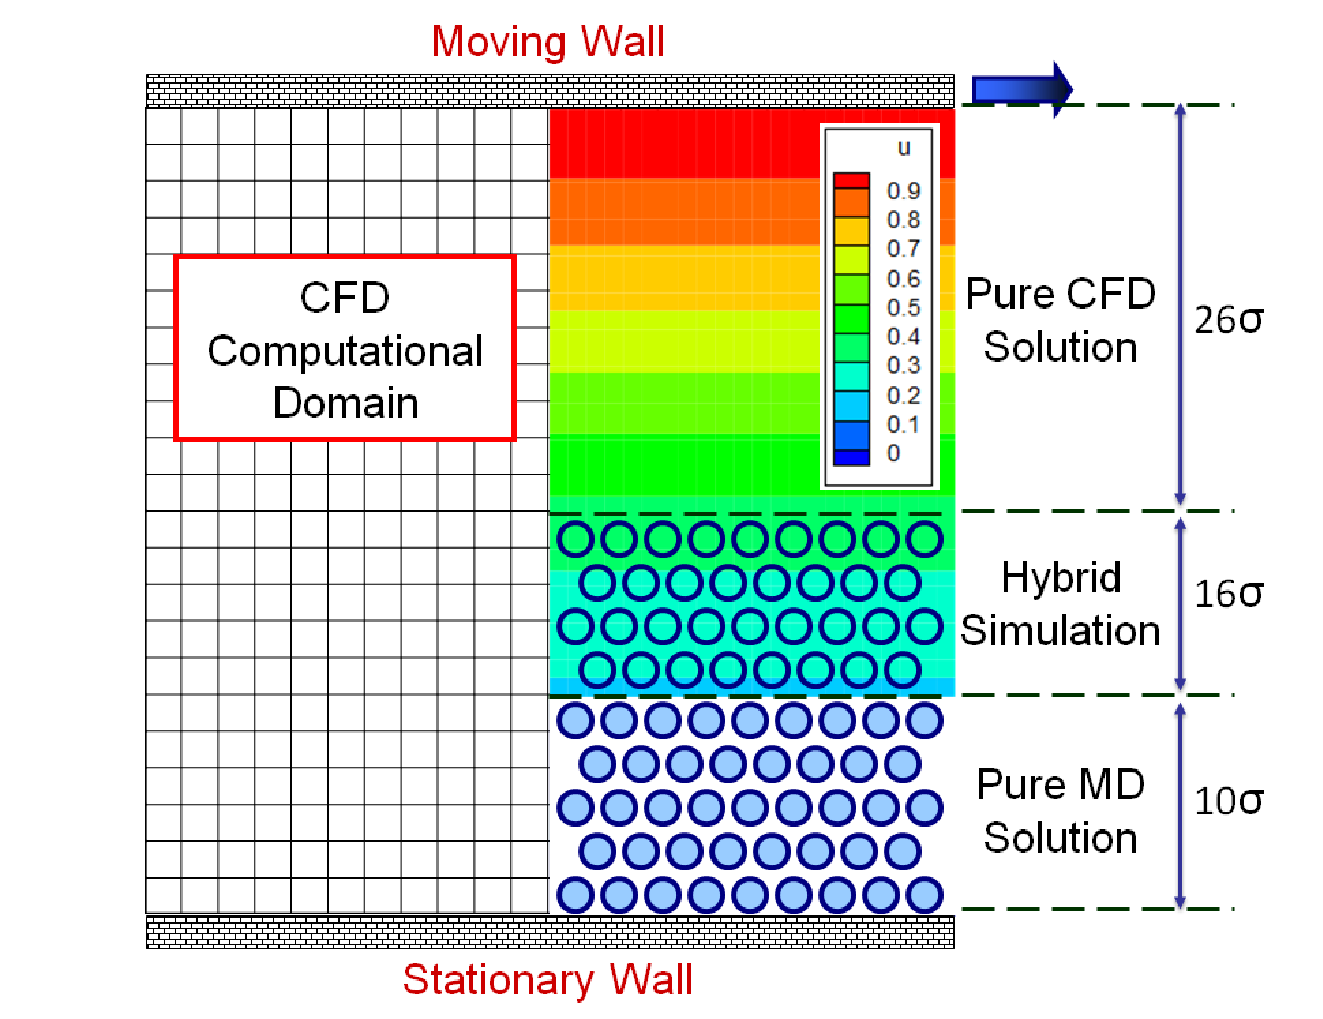
\includegraphics[width=0.8\linewidth]{Couette_Val_Domain.pdf}
\vskip-0.2cm
\caption{\small {\bf Computational domain of the Couette flow simulation.} The height of the fluid domain is 52$\sigma$ ($\approx$177$\AA$). CFD mesh size is 71$\times$27 and CFD cells at the pure MD region are treated as holes. MD domain size is about 140$\sigma$ in the X-direction and around 26$\sigma$ in the Y-direction, including the bottom wall. Periodic boundary condition is applied on the principal flow direction.}
\label{Couette_Val_Domain}
\end{figure}






%%%%% End Numerical Schemes %%%%%


%%%%% Numerical Solutions %%%%%
\section{Numerical Results}
\label{sec:result}

\subsection{Domain Construction and Validation}
\label{sec:result_val}

%The first problem is the Couette flow simulation, which have been in wide use for the validation of a hybrid CFD-MD solver.~\cite{Nie},\cite{Yen} We start from the validation case, which has 52$\sigma$ distance between two parallel plates and upper wall velocity is ${\sigma}/{\tau}$. We assume liquid argon particles are filled in the domain and both walls have artificial properties which is the same as those of liquid argon. Characteristic length of liquid argon is ${\sigma}=3.405{\times}10^{-10}$ and time scale is $\tau=2.2{\times}10^{-12}$. Density is $0.81m{\sigma}^{-3}$, which means 0.81 atoms are included in the characteristic volume.

%Table \ref{table:MD_Vel0} shows the averaged velocity on different layer size and sampling duration. Experiments were conducted with different system width changing from 35 $\sigma$ to 70 and 140 $\sigma$. From the individual test, we can find that increasing sampling duration or height of averaged layer does not linearly decrease the statistical error. At the first test, increasing the height of averaged layer from 0.1 $\sigma$ to 6.4 $\sigma$ reduces the statistical error by 4 times when sampling duration is 1 $\tau$ and this ratio even gets worse as sampling duration increases. The same situation also happens on sampling duration. Next, by comparing the first and third experiments, we find that the statistical error in general becomes half when the system size is 4 times bigger. This does not support the conclusion of statistical error analyses~\cite{Hadjicon2},\cite{Time_Mechanism} where the strength of error is inversely proportional to the system size. We assume that the upper and lower walls hinder the noise from being damped out. Nevertheless, increasing the system domain is more effective than numerically increasing the size of averaged layer in reducing the statistical error. Lastly, though not included in this table, we also conducted numbers of experiments by changing time step in MD simulation, $\Delta t_{MD}$. We could not find much difference in the strength of statistical noise with different time step and this concludes us that this fluctuation and its scale is physically natural phenomenon. So, time step for MD simulation is fixed as $\Delta t_{MD}=5 \times 10^3 \tau$ on all simulations.

%A sudden-start Couette flow is simulated to verify the accuracy of the current framework with a multiple replica sampling approach for the moderate-speed flow simulation. This application has been in widely used for the validation of a hybrid CFD-MD solver.~\cite{Nie,Yen} The flow is initially set at stationary and the upper wall starts moving in a constant velocity (1 $\sigma$/$\tau$). The physical boundary condition of the continuum domain governs the evolution of the whole flow field. Figure~\ref{Flat_Plate_Sol} presents a sudden-start Couette flow profile by CFD, MD and hybrid simulations. Although a slight fluctuation in the solution is observed, pure CFD produces an identically the same result as analytic solution and an MD simulation also describes the same flow physics though the slight fluctuation of the solution is observed. This verifies the accuracy of the individual solver. The hybrid solution also shows the slight deviation from the analytic solution, which is the fluctuation of the sampled MD solution. Nevertheless, the hybrid simulation succeeds in demonstrating the same flow physics as the analytic solution. This variation can even be diminished if the solution is visualized over a longer temporal range, which is observed in many articles.This proves that the current hybrid framework accurately analyzes the steady flow profile in nano-scaled systems.

A sudden-start Couette flow is simulated to verify the accuracy of the current framework with a multiple replica sampling approach for the moderate-speed flow simulation. This application has been widely used for the validation of a hybrid CFD-MD solver~\cite{Nie,Yen}. The flow is initially set at stationary and the upper wall starts moving in a constant velocity (1 $\sigma$/$\tau$). The physical boundary condition of the continuum domain governs the evolution of the whole flow field. Figure~\ref{Flat_Plate_Sol} presents a sudden-start Couette flow profile by CFD, MD, and hybrid simulations. Although a slight fluctuation in the solution is observed, pure CFD produces an identical result because an analytic solution and an MD simulation also describe the same flow physics. This result verifies the accuracy of the individual solver. The hybrid solution also shows a slight deviation from the analytic solution, which is the fluctuation of the sampled MD solution. Nevertheless, the hybrid simulation succeeds in demonstrating the same flow physics as the analytic solution. This variation can be diminished further if the solution is visualized over a longer temporal range, which has been observed in many previous studies. This capability proves that the current hybrid framework accurately analyzes the steady flow profile in nano-scaled systems.


%\begin{figure}[ht]
\begin{figure}
\centering
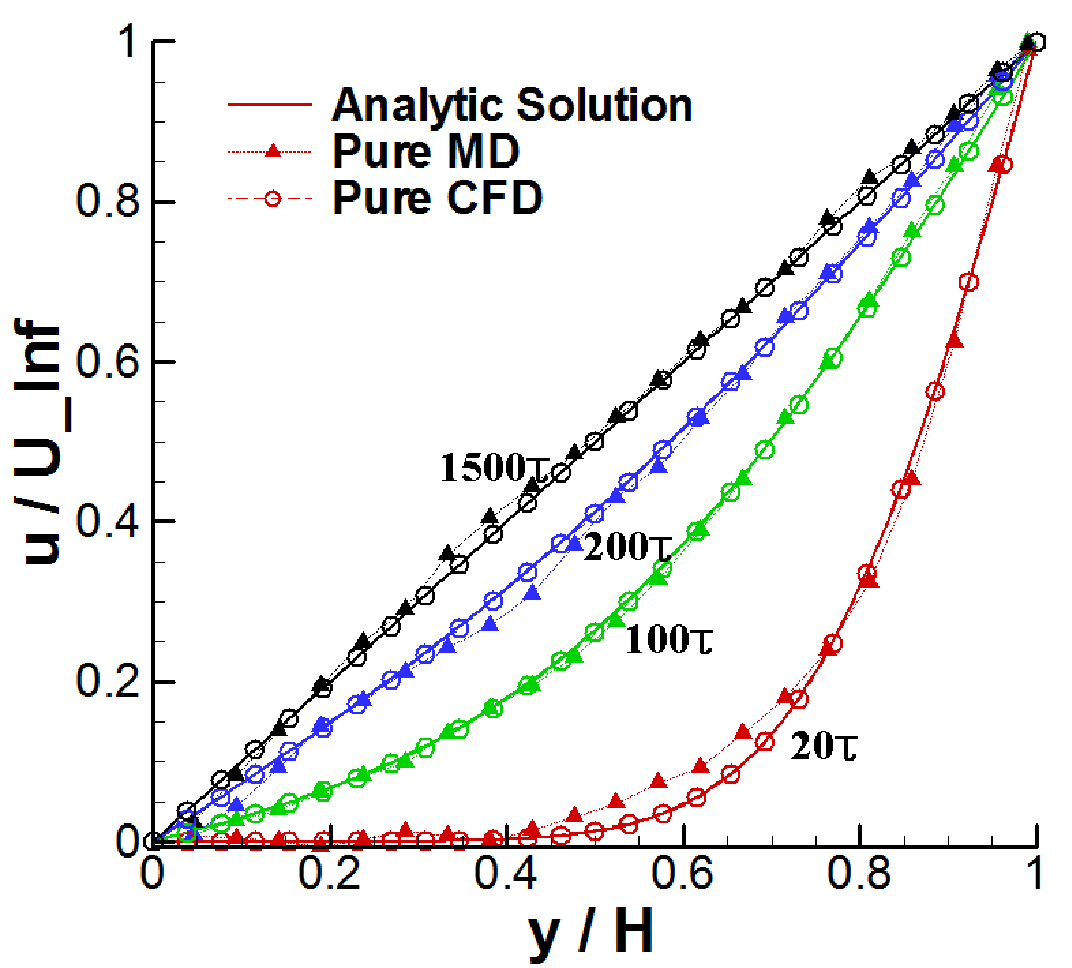
\includegraphics[width=0.6\linewidth]{Flat_Plate_Sol1.pdf}
\hskip 1cm
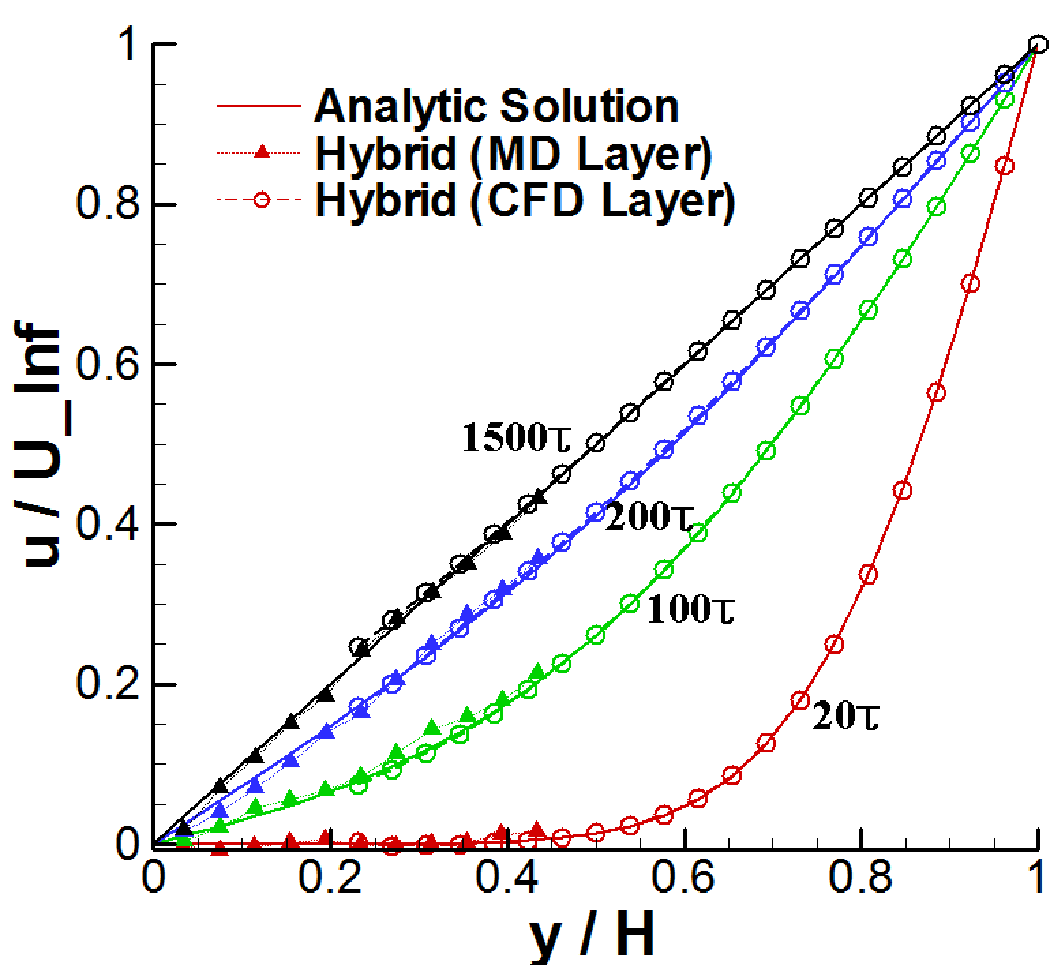
\includegraphics[width=0.6\linewidth]{Flat_Plate_Sol2.pdf}
\vskip-0.2cm
\caption{\small {\bf A time-accurate Couette flow profile.} The evolution of velocity field along the vertical direction is presented. CFD solution is the instantaneous profile at specified time and MD solution is spatially averaged over 2 $\sigma$ in height and temporally averaged for 1 sampling durations (=10$\tau$). (Left) Pure CFD solution is exactly the same as analytic solution. MD solution shows the same flow pattern as analytic solution, though some fluctuation is observed. This verifies that CFD and MD represents the same flow physics. (Right) The steady result by hybrid approach produces the same numerical result as analytic solution, though the slight time-lagging in the hybrid boundary is observed during the evolution.}
\label{Flat_Plate_Sol}
\end{figure}


%We now apply our framework on solving the flow field with 10$^{-7}$ meter scale. In this simulation, all conditions are identical to above simulation, except the height of the system becomes 10 times bigger (520$\sigma$) in height. As has been argued by Yen {\it{et al.}}~\cite{Yen}, the influence of thermal fluctuation becomes quite stronger in the simulation of the low shear rate flow, which can cause the unfavorable convergence characteristics. We believe that this numerical analysis at low shear rate condition evaluates the accuracy of our framework.

%Figure~\ref{Flat_Plate_Sol_L} shows the velocity profile of the Couette flow by a hybrid simulation compared with the analytic solution. Hybrid zone is composed of two layers for MDtoCFD boundary, one for buffer, two for CFDtoMD solution, another one buffer and one external force layer, starting from the bottom. The result by hybrid simulation is in good agreement with the analytic solution throughout the time domain, which evaluates the accuracy of our numerical implementation. Plotted results are instantaneous CFD solutions (MD solutions averaged over one sampling duration) without the filtering over a long physical time: this explains that the slight variation in steady-state solution is caused by the local fluctuation at that instance.


%%\begin{figure}[ht]
%\begin{figure}
%\centering
%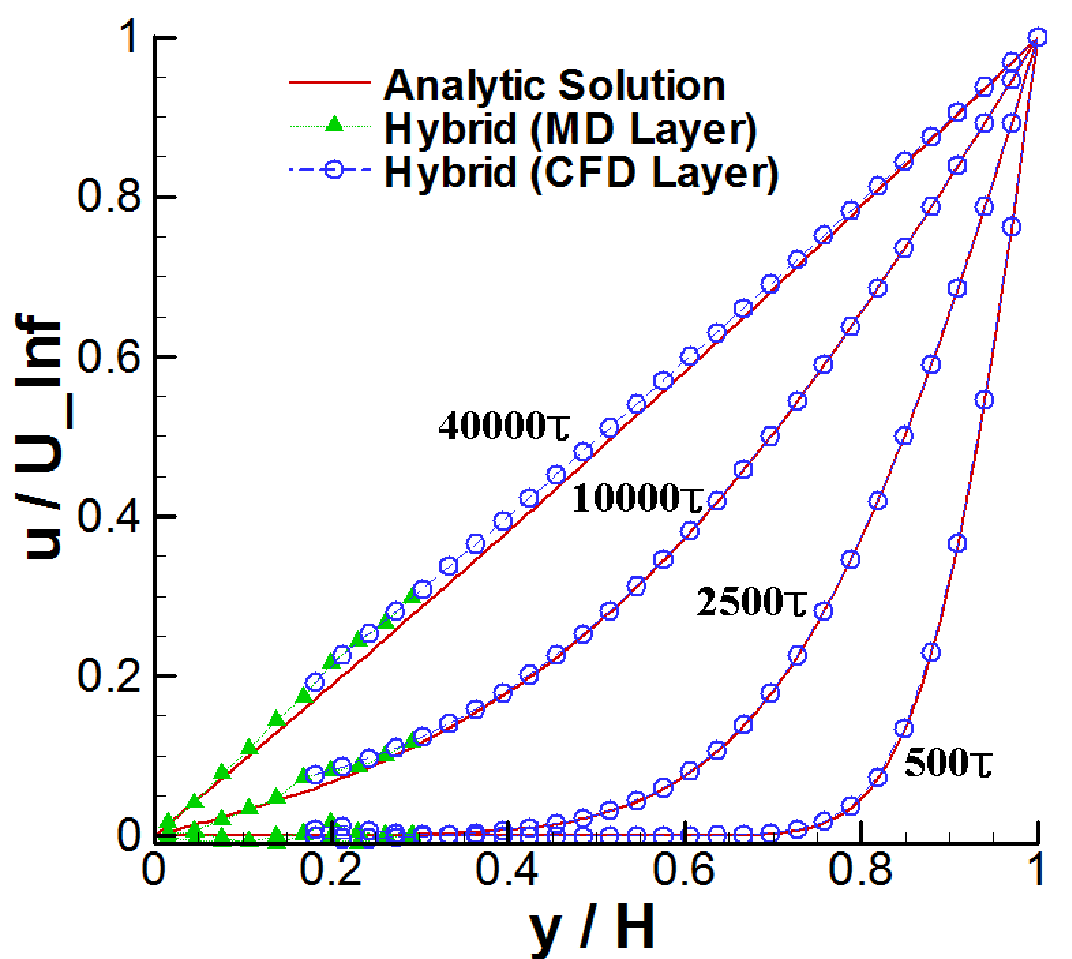
\includegraphics[width=0.6\linewidth]{Couette_Large.pdf}
%\vskip-0.2cm
%\caption{\small {\bf A Couette flow profile in O(100) nanometer domain.} The variation of non-dimensionalized horizontal velocity along the vertical direction is plotted . CFD solutions at each specified time and MD solutions averaged over 100 $\tau$ are compared with the analytic solution. Overall solutions match quite well with analytic solution.}
%\label{Flat_Plate_Sol_L}
%\end{figure}

%The flow condition in above experiment is rather unrealistic, which motivates us to apply the hybrid scheme to the analysis of moderate velocity flow. As has been expressed in Sec.~\ref{sec:numerical_lowspeed}, hybrid simulation of the low-speed flow field is mathematically possible but technically bound by the computing capacity, since the computational domain becomes $u^2$ times bigger in solving $1/u$ velocity field. We instead run $u^2$ independent simulations with the initial system size and different random number seeds in LAMMPS package. %A BigJob framework helps in scheduling multiple job execution and data management.

However, the flow condition in the above experiment is rather unrealistic, which motivates us to apply the hybrid scheme to the analysis of the moderate velocity flow. As discussed in Sec.~\ref{sec:numerical_noise}, the hybrid simulation of the low-speed flow field is mathematically possible but technically bound by the computing capacity, since the computational domain becomes $u^2$ times bigger in solving for a $1/u$ velocity field. Instead, we ran $u^2$ independent simulations with the initial system size and different random number seeds in the LAMMPS package.

%The Couette flow profiles with different numbers of samples are presented in Fig.~\ref{multiple_couette}. All configurations and parameters are identical to the above validation problem, except the upper plate velocity of 0.25 $\sigma/\tau$. Changing the velocity to 1/4 implies that averaging 16 samples are required to get the acceptable numerical solution. The result supports the above supposition. The solution becomes very accurate when 16 individual runs are sampled. The reduction of statistical noise by multiple replica sampling is clearly verified by the graph in Fig.~\ref{multiple_couette_temporal}. The noise is roughly seen to reduce by half with 4 times more samples and the solution of sampling 16 runs shows about 5 $\%$ of the noise compared to the analytic solution profile.

Fig.~\ref{multiple_couette} presents the Couette flow profiles with different numbers of samples. All configurations and parameters are identical to the above validation problem except the upper plate velocity of 0.25 $\sigma/\tau$.  Changing the velocity to 1/4 implies that an average of 16 samples is required to achieve an acceptable numerical solution. The result supports the above supposition. The solution becomes very accurate when 16 individual runs are sampled. The reduction of statistical noise by multiple replica samplings is clearly verified in the graph presented in Fig.~\ref{multiple_couette_temporal}. The noise is seen to reduce by roughly half with 4 times more samples. The solution of sampling 16 runs shows about 5$\%$ of the noise compared with the analytic solution profile.


%\begin{figure}[ht]
\begin{figure}
\centering
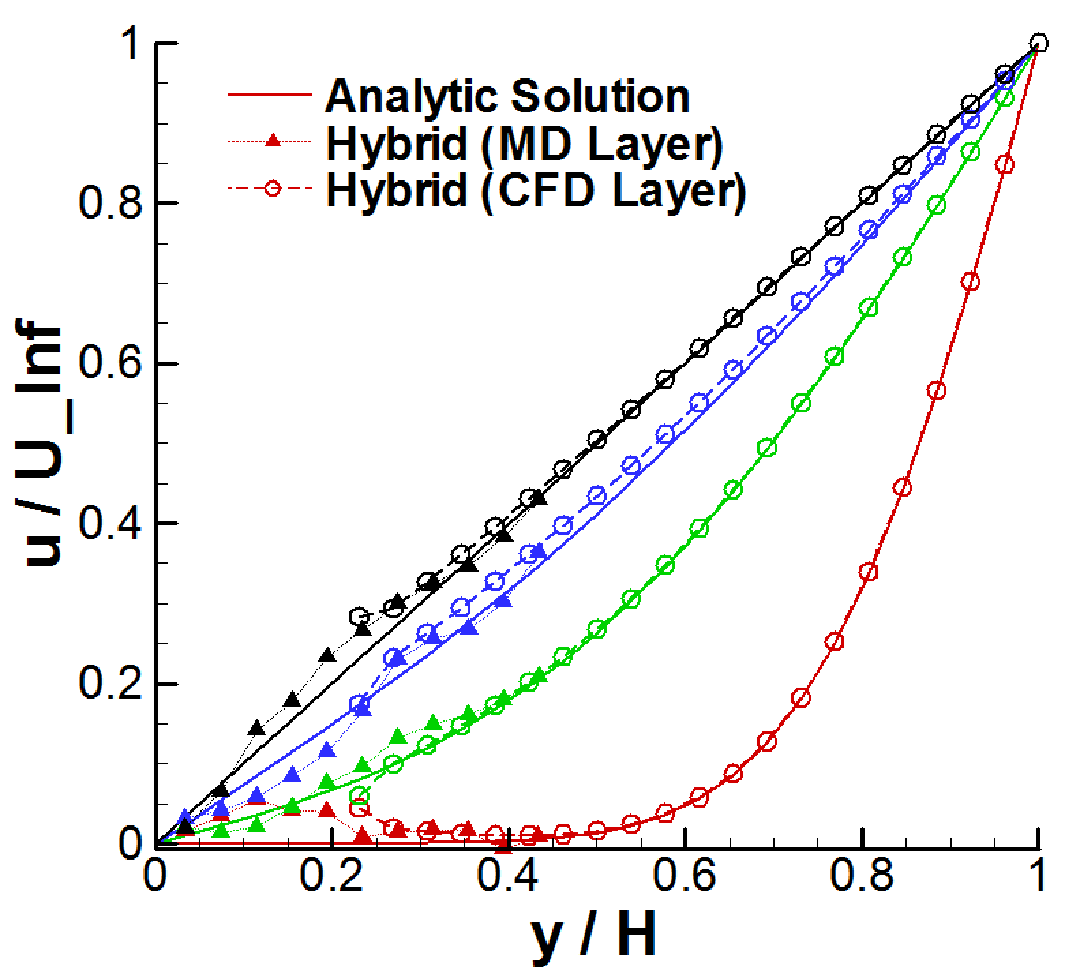
\includegraphics[width=0.6\linewidth]{Couette_025_Samp4.pdf}
\hskip 1cm
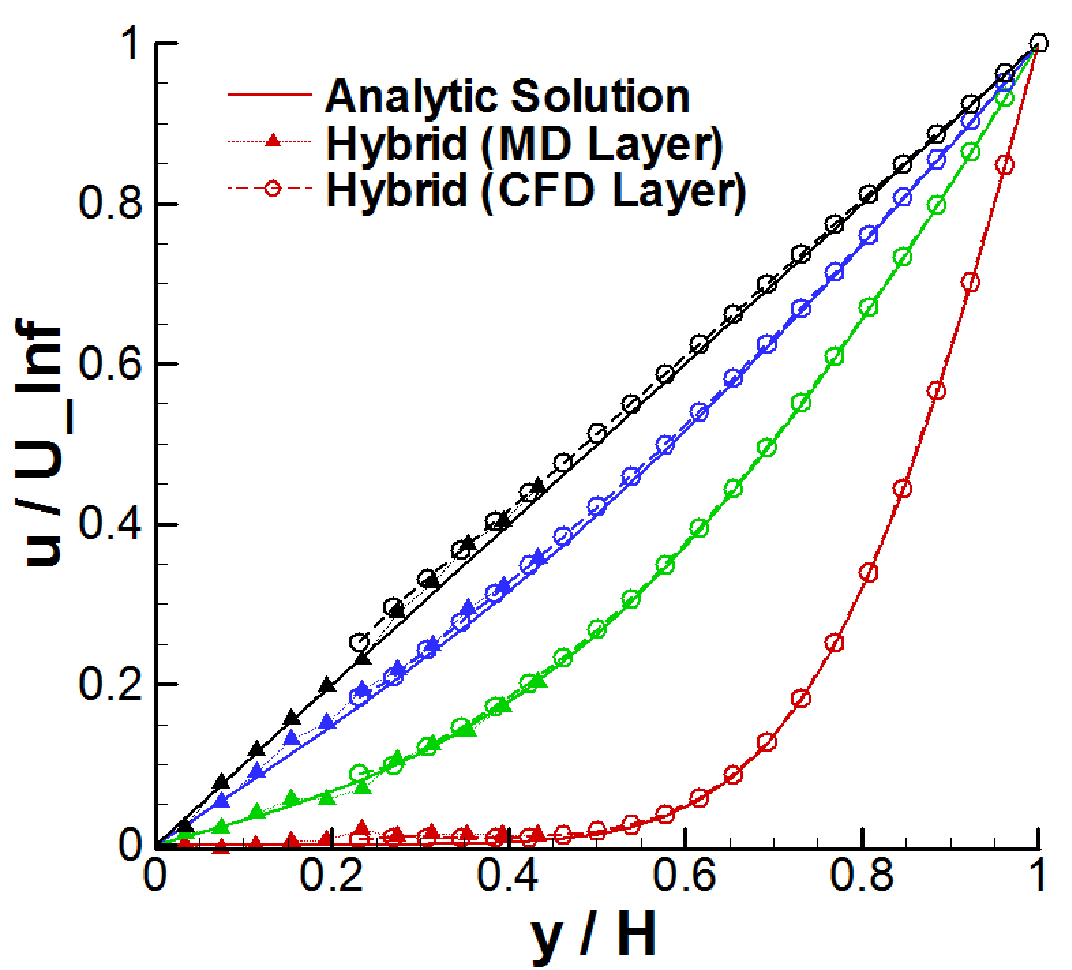
\includegraphics[width=0.6\linewidth]{Couette_025_Samp16.pdf}
\vskip-0.2cm
\caption{\small {\bf A Couette flow profile with the upper plate velocity of 0.25 $\sigma/\tau$.} The noisy solution when 4 individual simulations are averaged (left) is resolved by sampling 16 independent runs (right). Red lines denote the solution at 20 $\tau$; Green, blue and black lines are solutions at 100, 200 and 1500 $\tau$, respectively.}
\label{multiple_couette}
\end{figure}

\begin{figure}
\centering
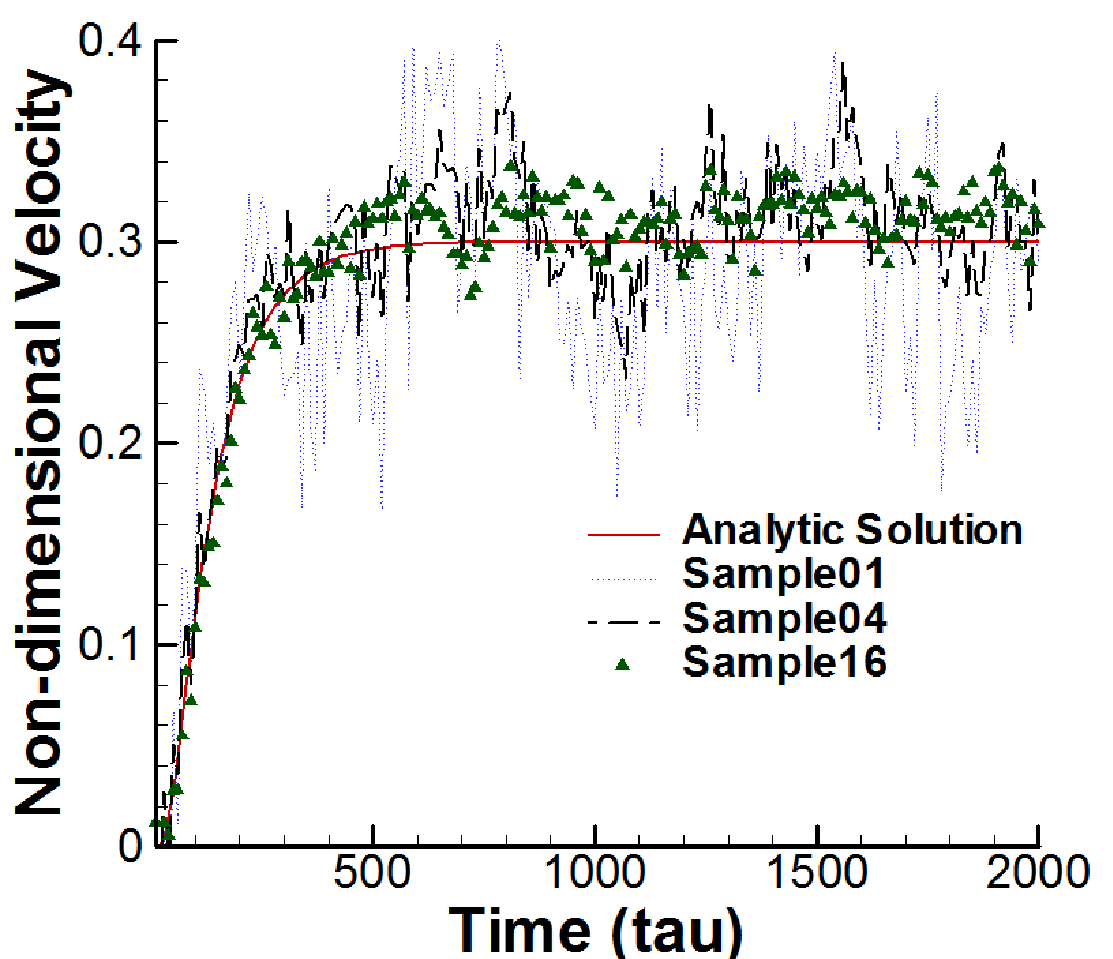
\includegraphics[width=0.6\linewidth]{Couette_025_Temporal_Multiset.pdf}
\vskip-0.2cm
\caption{\small {\bf The variation of continuum velocity in the middle of the overlapping region.} Velocity changes at various sampling runs are compared with the analytic solution. In case 16 simulations are averaged, the noise is about 5 $\%$ compared to the analytic solution.}
\label{multiple_couette_temporal}
\end{figure}


We compared the solution by multiple replica sampling is compared with the solution in the increased system domain. Figure~\ref{increase_system} shows the Couette flow profile with a 16 times larger system size in horizontal direction and the comparison of velocity variation in the middle of the overlapping region. From the result, both ways (multiple replica sampling and increasing system size) produce acceptable numerical solutions compared with the analytic solution. Interestingly, the scale of the noise compared with the analytic solution is very similar in both ways, which verifies that multiple replica sampling approach can replace  increasing the system size to reduce the statistical error.

%\begin{figure}[ht]
\begin{figure}
\centering
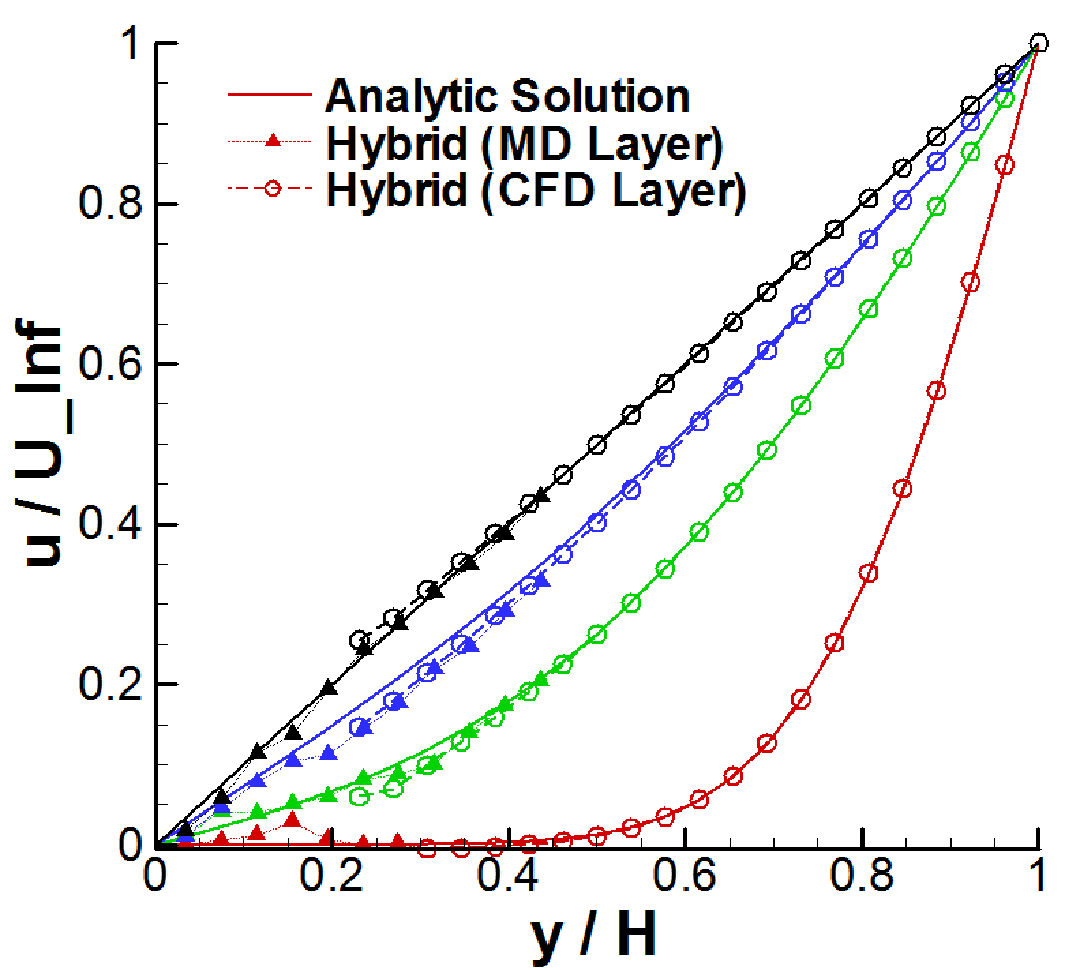
\includegraphics[width=0.6\linewidth]{Couette_025_Scale16.pdf}
\hskip 1cm
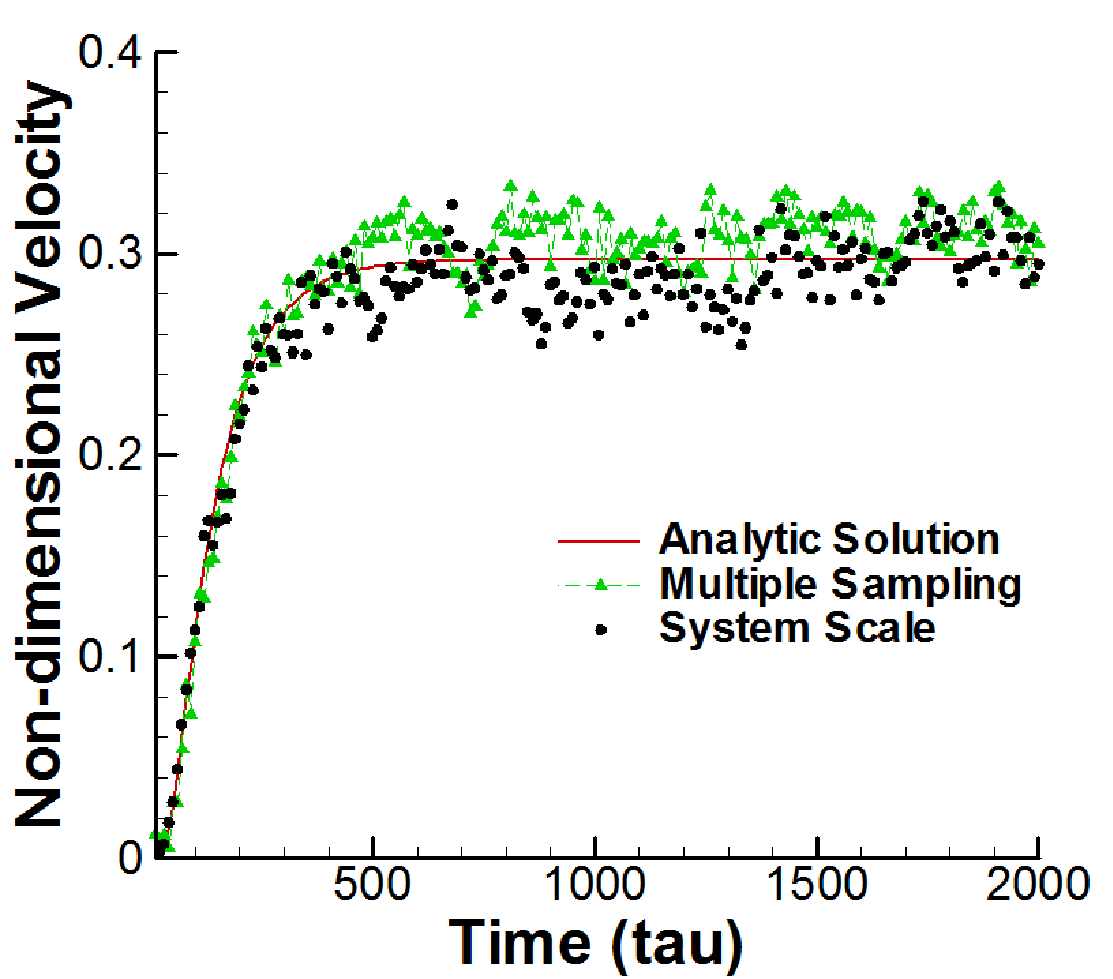
\includegraphics[width=0.6\linewidth]{Couette_025_Temporal_Multiset_VS_Scaleup.pdf}
\vskip-0.2cm
\caption{\small {\bf (Left) A Couette flow profile in increased system size.} 
Accurate flow profile can be obtained by increasing the system size 
16 times larger when the velocity is reduced to 1/4. Red lines denote 
the solution at 20 $\tau$; Green, blue and black lines are solutions 
at 100, 200 and 1500 $\tau$, respectively. 
{\bf (Right) The variation of the velocity in the middle of 
the overlapping region.} Solutions by multiple replica sampling 
and increasing the system contain the similar strength of the noise 
in the solution, which is around 5 $\%$ of analytic velocity profile. 
This implies that multiple replica sampling approach can replace 
the increase of system size for solving moderate velocity flow.}
\label{increase_system}
\end{figure}


Collectively, the results of multiple samples show the same order of accuracy compared with the increase in the system size. Particularly in cases where the physical system is large, multiple replica sampling is more effective than directly increasing the system size, because excessively large-scaled jobs (in view of wall-time limit or number of resources requested) are very hard allocate. In addition, the labor of manually submitting multiple independent runs and managing data sets can be relieved by adopting a BigJob framework.




\subsection{Transient Couette Flow Profiles in Multi-species and Polyatomic Fluids}
\label{sec:result_multi}

Contents

%%%%% End Numerical Solutions %%%%%


%%%%% Conclusion and Future Works %%%%%
\section{Conclusion and Future Works}
\label{sec:conclusion}


Accurate and efficient multi-scale flow simulations by a hybrid CFD-MD simulation framework have been presented in this paper. Constrained Lagrangian dynamics equations of motion and file-based hybrid interfaces are implemented on a highly-reliable LAMMPS molecular dynamics package and a verified in-house incompressible CFD code. They are virtually integrated as a single BigJob framework.

A number of numerical issues which harm the accuracy of a hybrid solution have been explored. First, quantifying the sampling noise from a stationary flow has been proposed as a way of determining coupling parameters. We argue that our simple and intuitive idea unveils the influence of individual coupling parameter on the magnitude of statistical error and is very cost-effective in contrast to traditional trial-and-error approach.
%until getting a stable solution.
Moreover, the empirical equation derived from the stationary flow simulation describes that well-know mathematical expressions on statistical error are not accurate on nano-scale wall-bounded systems.
Second, sampling multiple independent replicas has been introduced to refine the sampling noise of an individual solution and to explore to the low-speed flow regimes. This approach is superior to simulating a single large-scale problem set which is technically bound by computing capacity. The application to a Couette flow simulation in O(10) m/s velocity field is the first successful report of a moderate-speed flow simulation using a hybrid CFD-MD approach.
Last, a prediction-correction approach has been designed for the accurate unsteady simulation. This approach acquires better solution by enabling the imposition of interpolated hybrid boundary conditions. The application to the oscillating boundary problem expresses that the current approach diminishes the overshoot/undershoot phenomena in the conventional methods.

Along with numerical issues, computational issues for the efficient coupled simulations have been also discussed. We introduced a BigJob framework and this directly solves the co-scheduling problem among logically separated sub-tasks. A simple load-balancing function is also implemented on a BigJob framework, to achieve the load-balancing among those separated-yet-coupled codes. From numerical experiments, we evaluate that a BigJob is very powerful in reducing the waiting time of the coupled simulation. Also, a simple load-balancing function employed in a BigJob is effective in reducing the simulation runtime.

We emphasize that above numerical investigations ease the challenge to the hybrid simulation and broaden the application area. Also, our computational experiments contribute on how to efficiently conduct coupled simulations.



%The empirical mathematical equation on sampling noise has been presented in Sec.~\ref{sec:accuracy_conditions}. We argue that this is a refined model compared to previous mathematical expressions. However, the formulation has not been verified by various systems and conditions: coefficients will be changing according to the distance from the wall, characteristics of fluid and solid elements, etc. More rigorous research is required to address a globally acceptable equation of sampling noise.

Numerical simulations in Sec.~\ref{sec:accuracy} demonstrates that the delicate determination of coupling parameters along with the supplementary use of replica sampling approaches (in Sec.~\ref{sec:numerical_noise} is very important for the accurate hybrid simulations. Unfortunately, coupling conditions have been rather intuitively or empirically determined according to the flow physics of the target problem, and proposed mathematical expressions in statistical error~\cite{Hadjicon3,Time_Mechanism} fails to consider the variation of sampling noise depending on the geometric configuration. It is highly required to develop a mathematical model for predicting the sampling noise in wall-bounded flow systems.

Unsteady flow simulation in Sec.~\ref{sec:accuracy_oscillation} verifies that the prediction-correction approach provides more accurate solution than conventional temporal coupling scheme. The new approach is especially powerful in resolving the unfavorable overshoot/undershoot phenomena. On the other hand, the slight time-lagging effect in the conventional model has not been improved by the prediction-correction approach. We expect that this phenomenon can be resolved by applying higher-order extrapolation/interpolation on hybrid boundary regions.

%The unstable solution at Fig.~\ref{Couette_Noisy} represents the result of Couette flow simulation with 0.1 $\sigma / \tau$ upper plate velocity in O(100) nanometer system. The diverging solution is intuitively natural, according to the statistical noise measurement in Table~\ref{table:MD_Vel0_L}: the amount of statistical error is 25 percent of the steady-state velocity in MDtoCFD layer. For the worse, the signal-to-noise ratio is even larger at early stage. Thus the strong initial instability makes it harder for the solver to reach the steady-state solution. Increasing the sampling duration to 1000 $\tau$ did not help; increasing the height of layers implies the abandonment of hybrid method's merit over pure MD method.
%Clearly, this is one of the most important issues to make the family of hybrid methods a powerful tool which describes the detailed phenomena between solid obstacles and surrounding fluids more accurately. So far, two possible ways are observed at the first glance. First, setting the initial MD condition the same as steady-state CFD profile and starting hybrid simulation will, at least, alleviate the influence of noise at early stage. However, time-accurate unsteady solution can not be gained by this approach. Second, \skonote{check the clear term of zeta at Nie's formulation!} increasing $\zeta$ looks helpful in alleviating the noise in system level. However, this is worried whether excessive suppress of particles' vibration results in the breakup of fluid physics, i.e., breakup of energy conservation. A thorough investigation on the characteristics of statistical noise and design of numerical algorithm for acquiring the accurate solution without numerical damping are highly required.

%%\begin{figure}[ht!]
%\begin{figure}
%\centering
%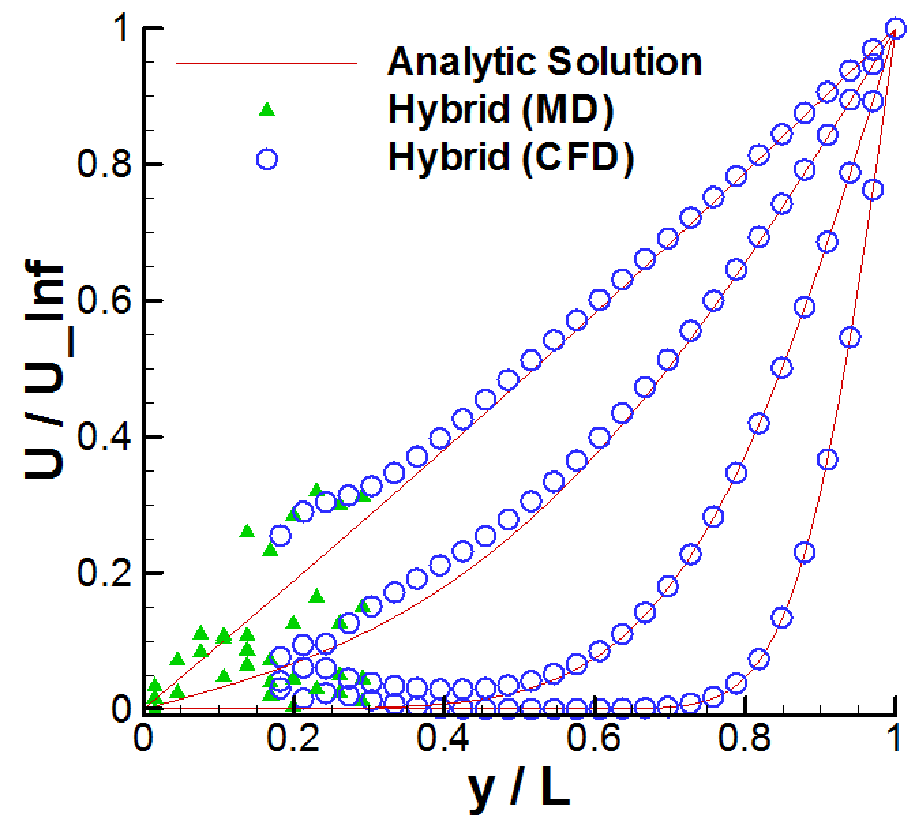
\includegraphics[width=0.6\linewidth]{Couette_Noisy.pdf}
%\vskip-0.2cm
%\caption{\small {\bf Unstable solution at low shear rate.} Velocity of the upper plate is 0.1 $\sigma / \tau$ and all other conditions are identical to the Couette flow simulation in large domain. The solution diverges at early stage, since the statistical error is very large compared to the hydrodynamic velocity.}
%\label{Stokes_Sol}
%\end{figure}



%%%%% End Conclusion and Future Works %%%%%


%%%%% Acknowledgement %%%%%
\section*{Acknowledgement}

Content

%%%%% End Acknowledgement %%%%%


% produces the bibliography section when processed by BibTeX
\bibliography{bibtex_database}
\bibliographystyle{aiaa}

\end{document}

% - Release $Name:  $ -
